%--------------------------------------
%ELECTROTECHNIQUE - SCHEMA DE LIAISON A LA TERRE
%--------------------------------------

%--------------------------------------
%appel de la classe de document et de ses options
%--------------------------------------

\documentclass[a4paper, 11pt, twoside, fleqn, french]{memoir}

\usepackage{AOCDTF}

\addbibresource{../../../parametres/bibliographies/bib_electrotechnique.bib}

%--------------------------------------
%données du document
%--------------------------------------

\title{\'Electrotechnique -- Schéma de liaison à la terre}
\date{\year}
\author[1]{Bruno Douchy}
%\author[2]{Prénom2 Nom2}
%\author[3]{Prénom3 Nom3}
%\author[4]{Prénom4 Nom4}

%--------------------------------------
%programmations spécifiques de mise-en-pages adaptables selon les matières et bibliographie
%--------------------------------------

%--------------------------------------
%CANEVAS
%--------------------------------------

\newcommand\BoxColor{\ifcase\thechapshift blue!30\or brown!30\or pink!30\or cyan!30\or green!30\or teal!30\or purple!30\or red!30\or olive!30\or orange!30\or lime!30\or gray!\or magenta!30\else yellow!30\fi} %définition de la couleur des marqueurs de chapitre

\newcounter{chapshift} %compteur de chapitre du marqueur de chapitre
\addtocounter{chapshift}{-1}
	
\newif\ifFrame %instruction conditionnelle pour les couleurs des pages
\Frametrue

\pagestyle{plain}

% the main command; the mandatory argument sets the color of the vertical box
\newcommand\ChapFrame{%
\AddEverypageHook{%
\ifFrame
\ifthenelse{\isodd{\value{page}}}
  {\backgroundsetup{contents={%
  \begin{tikzpicture}[overlay,remember picture]
  \node[
  	rounded corners=3pt,
    fill=\BoxColor,
    inner sep=0pt,
    rectangle,
    text width=1.5cm,
    text height=5.5cm,
    align=center,
    anchor=north west
  ] 
  at ($ (current page.north west) + (-0cm,-2*\thechapshift cm) $) %nombre négatif = espacement des marqueurs entre les différents chapitres (à régler en fin de rédaction) (4.5cm vaut un espacement équivalement à la hauteur du marqueur, une page peut en contenir 6 avec cet espacement-la mais il est le plus équilibré)
    {\rotatebox{90}{\hspace*{.5cm}%
      \parbox[c][1.2cm][t]{5cm}{%
        \raggedright\textcolor{black}{\sffamily\textbf{\leftmark}}}}};
  \end{tikzpicture}}}
  }
  {\backgroundsetup{contents={%
  \begin{tikzpicture}[overlay,remember picture]
  \node[
  	rounded corners=3pt,
    fill=\BoxColor,
    inner sep=0pt,
    rectangle,
    text width=1.5cm,
    text height=5.5cm,
    align=center,
    anchor=north east
  ] 
  at ($ (current page.north east) + (-0cm,-2*\thechapshift cm) $) %nombre négatif = espacement des marqueurs entre les différents chapitres (à régler en fin de rédaction) (4.5cm vaut un espacement équivalement à la hauteur du marqueur, une page peut en contenir 6 avec cet espacement-la mais il est le plus équilibré)
    {\rotatebox{90}{\hspace*{.5cm}%
      \parbox[c][1.2cm][t]{5cm}{%
        \raggedright\textcolor{black}{\sffamily\textbf{\leftmark}}}}};
  \end{tikzpicture}}}%
  }
  \BgMaterial%
  \fi%
}%
  \stepcounter{chapshift}
}

\renewcommand\chaptermark[1]{\markboth{\thechapter.~#1}{}} %redéfinition du marqueur de chapitre pour ne contenir que le titre du chapitre %à personnaliser selon le nombre de chapitre dans le cours

%\setVersion{0.1} %Sets the "official" version number.
\increaseBuild %Increases the build number at each build.

%à executer lorsqu'on souhaite un nouveau numéro de version du document

%--------------------------------------
%corps du document
%--------------------------------------

\begin{document} %corps du document

%--------------------------------------
%préface, page de couverture, table des matières...
%--------------------------------------

\frontmatter
	
\Framefalse %défini la booléenne Frame comme faux
	
	%--------------------------------------
	%page de couverture et de titre
	%--------------------------------------

	%--------------------------------------
%PRE-REQUIS
%--------------------------------------

%utiliser les environnement \begin{comment} \end{comment} pour mettre en commentaire le préambule une fois la programmation appelée dans le document maître (!ne pas oublier de mettre en commentaire \end{document}!)

\begin{comment}

\documentclass[a4paper, 11pt, twoside, fleqn]{memoir}

\usepackage{AOCDTF}

%--------------------------------------
%CANEVAS
%--------------------------------------

\newcommand\BoxColor{\ifcase\thechapshift blue!30\or brown!30\or pink!30\or cyan!30\or green!30\or teal!30\or purple!30\or red!30\or olive!30\or orange!30\or lime!30\or gray!\or magenta!30\else yellow!30\fi} %définition de la couleur des marqueurs de chapitre

\newcounter{chapshift} %compteur de chapitre du marqueur de chapitre
\addtocounter{chapshift}{-1}
	
\newif\ifFrame %instruction conditionnelle pour les couleurs des pages
\Frametrue

\pagestyle{plain}

% the main command; the mandatory argument sets the color of the vertical box
\newcommand\ChapFrame{%
\AddEverypageHook{%
\ifFrame
\ifthenelse{\isodd{\value{page}}}
  {\backgroundsetup{contents={%
  \begin{tikzpicture}[overlay,remember picture]
  \node[
  	rounded corners=3pt,
    fill=\BoxColor,
    inner sep=0pt,
    rectangle,
    text width=1.5cm,
    text height=5.5cm,
    align=center,
    anchor=north west
  ] 
  at ($ (current page.north west) + (-0cm,-2*\thechapshift cm) $) %nombre négatif = espacement des marqueurs entre les différents chapitres (à régler en fin de rédaction) (4.5cm vaut un espacement équivalement à la hauteur du marqueur, une page peut en contenir 6 avec cet espacement-la mais il est le plus équilibré)
    {\rotatebox{90}{\hspace*{.5cm}%
      \parbox[c][1.2cm][t]{5cm}{%
        \raggedright\textcolor{black}{\sffamily\textbf{\leftmark}}}}};
  \end{tikzpicture}}}
  }
  {\backgroundsetup{contents={%
  \begin{tikzpicture}[overlay,remember picture]
  \node[
  	rounded corners=3pt,
    fill=\BoxColor,
    inner sep=0pt,
    rectangle,
    text width=1.5cm,
    text height=5.5cm,
    align=center,
    anchor=north east
  ] 
  at ($ (current page.north east) + (-0cm,-2*\thechapshift cm) $) %nombre négatif = espacement des marqueurs entre les différents chapitres (à régler en fin de rédaction) (4.5cm vaut un espacement équivalement à la hauteur du marqueur, une page peut en contenir 6 avec cet espacement-la mais il est le plus équilibré)
    {\rotatebox{90}{\hspace*{.5cm}%
      \parbox[c][1.2cm][t]{5cm}{%
        \raggedright\textcolor{black}{\sffamily\textbf{\leftmark}}}}};
  \end{tikzpicture}}}%
  }
  \BgMaterial%
  \fi%
}%
  \stepcounter{chapshift}
}

\renewcommand\chaptermark[1]{\markboth{\thechapter.~#1}{}} %redéfinition du marqueur de chapitre pour ne contenir que le titre du chapitre %à personnaliser selon le nombre de chapitre dans le cours

%--------------------------------------
%corps du document
%--------------------------------------

\begin{document} %corps du document
	\openleft %début de chapitre à gauche

\end{comment}

\pagestyle{empty}

\begingroup

%--------------------------------------
%arrière-plan
%--------------------------------------
	\begin{tikzpicture}[remember picture, overlay]
		\begin{scope}[shift={(current page.south west)}]
			\draw[draw=lightgray,fill=lightgray] (0,0) rectangle (21,30);
		\end{scope}
	\end{tikzpicture}

%--------------------------------------
%bandeau vertical
%--------------------------------------

	\begin{tikzpicture}[remember picture, overlay]
		\begin{scope}[shift={(current page.south west)}]
			\draw[draw=orangelogo,fill=orangelogo, opacity=0.7] (0,0) rectangle (4,30);
		\end{scope}
	\end{tikzpicture}

%--------------------------------------
%texte dans bandeau vertical
%--------------------------------------
  
	\begin{tikzpicture}[remember picture, overlay]
	\begin{scope}[shift={(current page.south west)}]
			\draw (1.8,1) node [right, rotate=90, opacity=0.7] {\sffamily\textbf{\Large\color{bleulogo}M\'ETIERS DES TECHNOLOGIES ASSOCI\'EES}};
			\draw (2.5,1) node [right, rotate=90, opacity=0.7] {\sffamily\textbf{\Large\color{bleulogo}ASSOCIATION OUVRIÈRE DES COMPAGNONS DU DEVOIR ET DU TOUR DE FRANCE}};
			\draw (3.4,29) node [left, rotate=90, opacity=0.7] {\sffamily\textls[200]{\Huge\textbf{\color{bleulogo}BTS \'ELECTROTECHNIQUE}}};
		\end{scope}
	\end{tikzpicture}

%--------------------------------------
%titre 
%--------------------------------------

	\begin{tikzpicture}[remember picture, overlay]
		\begin{scope}[shift={(current page.north west)}]
		%\draw (5,-12.5) node [right] {\sffamily\textls[150]{\Huge\textbf{\color{darkgray}\textsc{Matière ligne1}}}}; 	%ligne 1 long intitulé de la matière
		\draw (5,-14) node [right, opacity=0.7] {\sffamily\textls[150]{\Huge\textbf{\color{bleulogo}Physique -- Chimie}}}; %intitulé de la matière
		\draw (20,-16) node [left, opacity=0.7] {\sffamily\textls[150]{\Huge\textbf{\color{bleulogo}Pré-requis}}}; %intitulé du cours
		%\draw (20,-17.5) node [left] {\sffamily\textls[150]{\Huge\textbf{\color{darkgray}\textsc{Cours ligne1}}}};  %ligne 1 long intitulé du cours
		\draw[very thick, orangelogo, opacity=0.7] (5,-15) -- (20,-15);
		\end{scope}
	\end{tikzpicture}

%--------------------------------------
%logo
%--------------------------------------

	\begin{tikzpicture}[remember picture, overlay]
		\begin{scope}[shift={(current page.north west)}]
			\draw (12.5,-7) %(12.5, -6) si long intitulé du chapitre
			node [opacity=0.3] {\includegraphics[scale=0.3]{logo_compagnons}};
			\draw (12.5,-23) %(12.5, -24) si long intitulé du chapitre
			node [opacity=0.3] {\includegraphics[scale=0.7]{logo_metier}};
		\end{scope}
	\end{tikzpicture}

\endgroup

\null\cleardoublepage

%\end{document}

	%--------------------------------------
%CANEVAS
%--------------------------------------

%utiliser les environnement \begin{comment} \end{comment} pour mettre en commentaire le préambule une fois la programmation appelée dans le document maître (!ne pas oublier de mettre en commentaire \end{document}!)

\begin{comment}

\documentclass[a4paper, 11pt, twoside, fleqn]{memoir}

\usepackage{AOCDTF}

%--------------------------------------
%CANEVAS
%--------------------------------------

\newcommand\BoxColor{\ifcase\thechapshift blue!30\or brown!30\or pink!30\or cyan!30\or green!30\or teal!30\or purple!30\or red!30\or olive!30\or orange!30\or lime!30\or gray!\or magenta!30\else yellow!30\fi} %définition de la couleur des marqueurs de chapitre

\newcounter{chapshift} %compteur de chapitre du marqueur de chapitre
\addtocounter{chapshift}{-1}
	
\newif\ifFrame %instruction conditionnelle pour les couleurs des pages
\Frametrue

\pagestyle{plain}

% the main command; the mandatory argument sets the color of the vertical box
\newcommand\ChapFrame{%
\AddEverypageHook{%
\ifFrame
\ifthenelse{\isodd{\value{page}}}
  {\backgroundsetup{contents={%
  \begin{tikzpicture}[overlay,remember picture]
  \node[
  	rounded corners=3pt,
    fill=\BoxColor,
    inner sep=0pt,
    rectangle,
    text width=1.5cm,
    text height=5.5cm,
    align=center,
    anchor=north west
  ] 
  at ($ (current page.north west) + (-0cm,-2*\thechapshift cm) $) %nombre négatif = espacement des marqueurs entre les différents chapitres (à régler en fin de rédaction) (4.5cm vaut un espacement équivalement à la hauteur du marqueur, une page peut en contenir 6 avec cet espacement-la mais il est le plus équilibré)
    {\rotatebox{90}{\hspace*{.5cm}%
      \parbox[c][1.2cm][t]{5cm}{%
        \raggedright\textcolor{black}{\sffamily\textbf{\leftmark}}}}};
  \end{tikzpicture}}}
  }
  {\backgroundsetup{contents={%
  \begin{tikzpicture}[overlay,remember picture]
  \node[
  	rounded corners=3pt,
    fill=\BoxColor,
    inner sep=0pt,
    rectangle,
    text width=1.5cm,
    text height=5.5cm,
    align=center,
    anchor=north east
  ] 
  at ($ (current page.north east) + (-0cm,-2*\thechapshift cm) $) %nombre négatif = espacement des marqueurs entre les différents chapitres (à régler en fin de rédaction) (4.5cm vaut un espacement équivalement à la hauteur du marqueur, une page peut en contenir 6 avec cet espacement-la mais il est le plus équilibré)
    {\rotatebox{90}{\hspace*{.5cm}%
      \parbox[c][1.2cm][t]{5cm}{%
        \raggedright\textcolor{black}{\sffamily\textbf{\leftmark}}}}};
  \end{tikzpicture}}}%
  }
  \BgMaterial%
  \fi%
}%
  \stepcounter{chapshift}
}

\renewcommand\chaptermark[1]{\markboth{\thechapter.~#1}{}} %redéfinition du marqueur de chapitre pour ne contenir que le titre du chapitre %à personnaliser selon le nombre de chapitre dans le cours

%--------------------------------------
%corps du document
%--------------------------------------

\begin{document} %corps du document
	\openleft %début de chapitre à gauche

\end{comment}

\pagestyle{empty}
\thispagestyle{empty}

\begingroup

%--------------------------------------
%logo Compagnon
%--------------------------------------
 
\begin{tikzpicture}[remember picture, overlay]
	\begin{scope}[shift={(current page.north west)}]
		\draw (2.5,-1)
		node [below right]{\includegraphics[scale=0.1]{logo_compagnons_nom.png}};
	\end{scope}
\end{tikzpicture}

~\\[5cm] %espace insécable pour marquer le début du texte sur l'environnement et situer d'autres éléments de texte sur la page

%--------------------------------------
%titre de la page
%--------------------------------------

\begin{flushleft}
	\HUGE\sffamily\textbf{\'Electrotechnique}\\
\end{flushleft}
\HRule
\begin{flushright}
	\huge\sffamily\textbf{Schéma de liaison à la terre}\\[0.4cm]
\end{flushright}
~\\[2cm]

%--------------------------------------
%auteur et logo MTA
%--------------------------------------

\begin{minipage}{0.3\textwidth}
 \noindent\large
		\rmfamily Bruno \textsc{Douchy}
%		\\
%		\rmfamily Prénom2 \textsc{Nom2}
\end{minipage}
\hfill
\begin{minipage}{0.3\textwidth}
	\centering
	\includegraphics[scale=0.25]{logo_metier.png}
\end{minipage}

\begin{comment}
\hfill
\begin{minipage}{0.3\textwidth}
	\begin{flushright} \large
		\rmfamily Prénom3 \textsc{Nom3} %auteur supplémentaires à rajouter en mettant en commentaire l'environnement comment
		\\
 		\rmfamily Prénom4 \textsc{Nom4}
	\end{flushright}
\end{minipage}
\end{comment}

\vfill
\begin{flushleft}
	\sffamily\bfseries\large\ Édition \the\year.\the\month
	\\
	~v\version
\end{flushleft}
\vfill

%--------------------------------------
%pied de page Compagnon
%--------------------------------------

\begin{tikzpicture}[remember picture, overlay]
	\begin{scope}[shift={(current page.south west)}]
		\draw (2.5,1)
		node [above right]{\includegraphics{pied_page_compagnons.png}};
	\end{scope}
\end{tikzpicture}

\endgroup
\null\clearpage

%\end{document}

	\pagestyle{plain} %style de page avec en-tête et pied-de-page
	\pagenumbering{roman}
	\openany

	%--------------------------------------
	%listes de contenus
	%--------------------------------------
	
	{\hypersetup{linkcolor=black}\tableofcontents} %table des matières en noir
	\newpage
	{\hypersetup{linkcolor=black}\listoftables} %liste des tableaux en noir
	\newpage
	{\hypersetup{linkcolor=black}\listoffigures} %liste des figures en noir
	{\hypersetup{linkcolor=black}\listtheoremname\listtheorems{formule}} %liste des équations en noir
	{\hypersetup{linkcolor=black}\listdefinitionname\listtheorems{definition}} %liste des définitions en noir
	{\hypersetup{linkcolor=black}\listexemplename\listtheorems{exemple}} %liste des définitions en noir

	\openright %début de chapitre à "droite" mais comme demarrage de la numérotation inversé avec la page de titre, ça décale l'ouverture des chapitre à gauche

	%--------------------------------------
	%chapitre d'introduction
	%--------------------------------------

%--------------------------------------
%corps de texte, annexes
%--------------------------------------

\mainmatter

\Frametrue %défini la booléenne Frame comme vrai -> marqueurs de chapitre

	%--------------------------------------
	%inclusion des chapitres
	%--------------------------------------

	%--------------------------------------
%ELECTROTECHNIQUE - SCHEMA DE LIAISON A LA TERRE
%--------------------------------------

%utiliser les environnement \begin{comment} \end{comment} pour mettre en commentaire le préambule une fois la programmation appelée dans le document maître (!ne pas oublier de mettre en commentaire \end{document}!)

\begin{comment}

\documentclass[a4paper, 11pt, twoside, fleqn]{memoir}

\usepackage{AOCDTF}

%--------------------------------------
%CANEVAS
%--------------------------------------

\newcommand\BoxColor{\ifcase\thechapshift blue!30\or brown!30\or pink!30\or cyan!30\or green!30\or teal!30\or purple!30\or red!30\or olive!30\or orange!30\or lime!30\or gray!\or magenta!30\else yellow!30\fi} %définition de la couleur des marqueurs de chapitre

\newcounter{chapshift} %compteur de chapitre du marqueur de chapitre
\addtocounter{chapshift}{-1}
	
\newif\ifFrame %instruction conditionnelle pour les couleurs des pages
\Frametrue

\pagestyle{plain}

% the main command; the mandatory argument sets the color of the vertical box
\newcommand\ChapFrame{%
\AddEverypageHook{%
\ifFrame
\ifthenelse{\isodd{\value{page}}}
  {\backgroundsetup{contents={%
  \begin{tikzpicture}[overlay,remember picture]
  \node[
  	rounded corners=3pt,
    fill=\BoxColor,
    inner sep=0pt,
    rectangle,
    text width=1.5cm,
    text height=5.5cm,
    align=center,
    anchor=north west
  ] 
  at ($ (current page.north west) + (-0cm,-2*\thechapshift cm) $) %nombre négatif = espacement des marqueurs entre les différents chapitres (à régler en fin de rédaction) (4.5cm vaut un espacement équivalement à la hauteur du marqueur, une page peut en contenir 6 avec cet espacement-la mais il est le plus équilibré)
    {\rotatebox{90}{\hspace*{.5cm}%
      \parbox[c][1.2cm][t]{5cm}{%
        \raggedright\textcolor{black}{\sffamily\textbf{\leftmark}}}}};
  \end{tikzpicture}}}
  }
  {\backgroundsetup{contents={%
  \begin{tikzpicture}[overlay,remember picture]
  \node[
  	rounded corners=3pt,
    fill=\BoxColor,
    inner sep=0pt,
    rectangle,
    text width=1.5cm,
    text height=5.5cm,
    align=center,
    anchor=north east
  ] 
  at ($ (current page.north east) + (-0cm,-2*\thechapshift cm) $) %nombre négatif = espacement des marqueurs entre les différents chapitres (à régler en fin de rédaction) (4.5cm vaut un espacement équivalement à la hauteur du marqueur, une page peut en contenir 6 avec cet espacement-la mais il est le plus équilibré)
    {\rotatebox{90}{\hspace*{.5cm}%
      \parbox[c][1.2cm][t]{5cm}{%
        \raggedright\textcolor{black}{\sffamily\textbf{\leftmark}}}}};
  \end{tikzpicture}}}%
  }
  \BgMaterial%
  \fi%
}%
  \stepcounter{chapshift}
}

\renewcommand\chaptermark[1]{\markboth{\thechapter.~#1}{}} %redéfinition du marqueur de chapitre pour ne contenir que le titre du chapitre %à personnaliser selon le nombre de chapitre dans le cours

%--------------------------------------
%corps du document
%--------------------------------------

\begin{document} %corps du document
	\openleft %début de chapitre à gauche

\end{comment}

\chapter{Les dangers de l'électricité}
\label{chap:dangers_electricite}
\ChapFrame %appel du marqueur de chapitre

\section{Catégories de tension}

\begin{table}[h]
\caption{Domaines de tensions\label{tab:categories_tension}}
\begin{threeparttable} %note dans tableau
\begin{tabularx}{\textwidth}{l C k@{${\enspace{}}U_n{\enspace{}}$}i k@{${\enspace{}}U_n{\enspace{}}$}i} %les deux derniers,types de colonne sont deux colonnes compactées avec la lettre U comme colonne du centre
\toprule
\multicolumn{2}{c}{\thead{Domaine de tension}}	& \multicolumn{2}{c}{\thead[c]{Courant alternatif\tnote{\ 1}}}		&  \multicolumn{2}{c}{\thead[c]{Courant continu}} \\
\midrule
Très Basse Tension										& TBT		&						& \leq 50\volt				& 						& \leq 120\volt \\
Basse Tension												& BT			& 50\volt < 		& \leq 1000\volt			& 120\volt < 		& \leq 1500\volt \\
\multirow[t]{2}{*}{Haute Tension\tnote{2}}	& HTA		& 1000\volt < 	& \leq 50\kilo\volt		& 1500\volt < 	& \leq 75\kilo\volt \\
																	& HTB		&  					& > 50\kilo\volt			& 						& > 75\kilo\volt \\
\bottomrule
\end{tabularx}
\begin{tablenotes}
    \item[1] Tension nominale exprimée en \emph{valeur efficace} $U_n$\,;
    \item[2] Les basses tensions ne sont plus divisées en deux catégories depuis 2010, seule la haute tension conserve cette caractéristique.
\end{tablenotes}
\end{threeparttable}
\end{table}
	
\section{Action du courant électrique sur le corps humain}

Les dégâts provoqués au corps humain par un choc électrique sont directement corrélés à l'énergie dissipée par ce choc. Cette énergie dissipée est définie par la \emph{loi de Joule}.

\begin{formule}[Loi de Joule]
\begin{align}
		W &= R \cdot I^{2} \cdot t
\end{align}
\end{formule}

\begin{textvariables}
R						& résistance										& ohm 						& \ohm								&\\
I						& courant électrique							& milliampère			& \milli\ampere					& \\
t						& durée												& seconde					& \second							&	\\
\end{textvariables}

La présence d'une tension électrique entraine toujours un risque de choc électrique mais il est peu aisé de déterminer un seuil de tension pour lequel le choc est dangereux car ce sont l'\emph{intensité} du courant $I$ traversant le corps et la \emph{durée} $t$ du choc électrique qui permettent de déterminer la probabilité de décès.\\

\begin{formule}[Probabilité d'électrocution]
\begin{align}
		I &= \frac{116}{\sqrt{t}}
\end{align}
\end{formule}

\begin{textvariables}
I						& courant électrique							& milliampère			& \milli\ampere					& 	Courant traversant le corps 	\\
t						& durée												& seconde					& \second							& 	Durée du choc électrique d'une durée ($8\milli\second < t \leq 5\second \nonumber$) \\
116					& constante										& / 							& 	/									& 	Constante empirique déterminée statistiquement\supercite{WildiSybille2014}\\
\end{textvariables}

En plus de l'intensité du courant et de la durée de passage du courant dans le corps, la surface de contact et la susceptibilité spécifique à chaque personne sont d'autres facteurs de gravité d'un contact électrique. Plus de précisions sur la prévention du danger électrique en \superref{sec:etat_lieux_prevention_electrique}.

\subsection{Effet du courant alternatif}

Les effets du courant alternatif entre \SI{15}{\hertz} et \SI{100}{\hertz} sont décrit en \autoref{fig:effets_courant_electrique_alternatif}. 

%--------------------------------------
%ELECTROTECHNIQUE - SCHEMA DE LIAISON A LA TERRE
%--------------------------------------

%utiliser les environnement \begin{comment} \end{comment} pour mettre en commentaire le préambule une fois la programmation appelée dans le document maître (!ne pas oublier de mettre en commentaire \end{document}!)

\begin{comment}

\documentclass[a4paper, 11pt, twoside, fleqn]{memoir}

\usepackage{AOCDTF}

%--------------------------------------
%CANEVAS
%--------------------------------------

\newcommand\BoxColor{\ifcase\thechapshift blue!30\or brown!30\or pink!30\or cyan!30\or green!30\or teal!30\or purple!30\or red!30\or olive!30\or orange!30\or lime!30\or gray!\or magenta!30\else yellow!30\fi} %définition de la couleur des marqueurs de chapitre

\newcounter{chapshift} %compteur de chapitre du marqueur de chapitre
\addtocounter{chapshift}{-1}
	
\newif\ifFrame %instruction conditionnelle pour les couleurs des pages
\Frametrue

\pagestyle{plain}

% the main command; the mandatory argument sets the color of the vertical box
\newcommand\ChapFrame{%
\AddEverypageHook{%
\ifFrame
\ifthenelse{\isodd{\value{page}}}
  {\backgroundsetup{contents={%
  \begin{tikzpicture}[overlay,remember picture]
  \node[
  	rounded corners=3pt,
    fill=\BoxColor,
    inner sep=0pt,
    rectangle,
    text width=1.5cm,
    text height=5.5cm,
    align=center,
    anchor=north west
  ] 
  at ($ (current page.north west) + (-0cm,-2*\thechapshift cm) $) %nombre négatif = espacement des marqueurs entre les différents chapitres (à régler en fin de rédaction) (4.5cm vaut un espacement équivalement à la hauteur du marqueur, une page peut en contenir 6 avec cet espacement-la mais il est le plus équilibré)
    {\rotatebox{90}{\hspace*{.5cm}%
      \parbox[c][1.2cm][t]{5cm}{%
        \raggedright\textcolor{black}{\sffamily\textbf{\leftmark}}}}};
  \end{tikzpicture}}}
  }
  {\backgroundsetup{contents={%
  \begin{tikzpicture}[overlay,remember picture]
  \node[
  	rounded corners=3pt,
    fill=\BoxColor,
    inner sep=0pt,
    rectangle,
    text width=1.5cm,
    text height=5.5cm,
    align=center,
    anchor=north east
  ] 
  at ($ (current page.north east) + (-0cm,-2*\thechapshift cm) $) %nombre négatif = espacement des marqueurs entre les différents chapitres (à régler en fin de rédaction) (4.5cm vaut un espacement équivalement à la hauteur du marqueur, une page peut en contenir 6 avec cet espacement-la mais il est le plus équilibré)
    {\rotatebox{90}{\hspace*{.5cm}%
      \parbox[c][1.2cm][t]{5cm}{%
        \raggedright\textcolor{black}{\sffamily\textbf{\leftmark}}}}};
  \end{tikzpicture}}}%
  }
  \BgMaterial%
  \fi%
}%
  \stepcounter{chapshift}
}

\renewcommand\chaptermark[1]{\markboth{\thechapter.~#1}{}} %redéfinition du marqueur de chapitre pour ne contenir que le titre du chapitre %à personnaliser selon le nombre de chapitre dans le cours

%--------------------------------------
%corps du document
%--------------------------------------

\begin{document} %corps du document
	\openleft %début de chapitre à gauche

\end{comment}

\begin{figure}[H]
\centering
\caption{Effets du courant alternatif sur le corps humain \label{fig:effets_courant_electrique_alternatif}}
\begin{tikzpicture}
%\DrawGrid{(-7,-5)}{(7,5)} %grille d'aide pour le placement des objets

\draw (-7,4) node [right, minimum width=2cm, text width=1.8cm] {\footnotesize{Intensité de contact $I_c$}};
\draw [->] (-5,2.2) -- (-5,4);
\draw (-5, 2) node {\vdots};
\draw (-5,-3.9) -- (-5,1.6);

\draw (-5.4,-3) node [left] {\SI{0,5}{\milli\ampere}};
\draw [->] (-5.2,-3) -- (-4.5,-3);
\draw (-4.2,-3) node [anchor=mid west, text width=7cm] (A) {Sensation de picotements, de très faible à faible};
\draw (7,-3.5) node [anchor=east] {\includegraphics[width=2cm]{sensation}};

\draw (-5.4,-2.6) node [left] {\SI{10}{\milli\ampere}};
\draw [->] (-5.2,-2.6) -- (-4.5,-2.6);
\draw (-4.2,-2.6) node [anchor=mid west, text width=7cm] {Seuil de non lâcher, paralysie musculaire};
\draw (3.2,-2.6) node [anchor=west] {\includegraphics[width=1.5cm]{tetanisation}};

\draw (-5.4,-1.8) node [left] {\SI{30}{\milli\ampere}};
\draw [->] (-5.2,-1.8) -- (-4.5,-1.8);
\draw (-4.2,-1.8) node [anchor=mid west, text width=7cm] {Seuil de paralysie respiratoire};
\draw (7,-1.8) node [anchor=east] {\includegraphics[width=1.5cm]{paralysie_poumon}};

\draw (-5.4,0.7) node [left] {\SI{75}{\milli\ampere}};
\draw [->] (-5.2,0.7) -- (-4.5,0.7);
\draw (-4.2,0.7) node [anchor=mid west, text width=7cm] {Seuil de fibriliation ventriculaire};
\draw (5.1,0.7) node {\includegraphics[width=1.5cm]{fibrillation}};

\draw (-5.4,3.1) node [left] {\SI{1}{\ampere}};
\draw [->] (-5.2,3.1) -- (-4.5,3.1);
\draw (-4.2,3.1) node [anchor=mid west, text width=7cm] {Arrêt du coeur};
\draw (5.2,3.1) node {\includegraphics[width=2.4cm]{arret_cardiaque}};

\end{tikzpicture}
\end{figure}

%\end{document}

\subsubsection{Cas particuliers}

Pour le courant alternatifs d'une fréquence supérieures à \SI{100}{\hertz} :

\begin{itemize}
\item Plus la fréquence du courant augmente, plus les risques de fibrillation ventriculaire diminue\,;
\item Plus la fréquence du courant augmente, plus les risques de brûlures augmentent\,;
\item Plus la fréquence du courant augmente, plus l'impédance du corps humain diminue\,;
\item Il est généralement considéré que les conditions de protection contre les contacts indirects sont identiques que ça soit sous une fréquence de \SI{50}{\hertz} (réseau électrique domestique en Europe) où \SI{400}{\hertz} (réseau électrique des bateaux, avions, batmobile\ldots).
\end{itemize}

\subsection{Effet du courant continu}

Les effets du courant continus sont décrits en \autoref{fig:effets_courant_electrique_continu}.

%--------------------------------------
%ELECTROTECHNIQUE - SCHEMA DE LIAISON A LA TERRE
%--------------------------------------

%utiliser les environnement \begin{comment} \end{comment} pour mettre en commentaire le préambule une fois la programmation appelée dans le document maître (!ne pas oublier de mettre en commentaire \end{document}!)

\begin{comment}

\documentclass[a4paper, 11pt, twoside, fleqn]{memoir}

\usepackage{AOCDTF}

%--------------------------------------
%CANEVAS
%--------------------------------------

\newcommand\BoxColor{\ifcase\thechapshift blue!30\or brown!30\or pink!30\or cyan!30\or green!30\or teal!30\or purple!30\or red!30\or olive!30\or orange!30\or lime!30\or gray!\or magenta!30\else yellow!30\fi} %définition de la couleur des marqueurs de chapitre

\newcounter{chapshift} %compteur de chapitre du marqueur de chapitre
\addtocounter{chapshift}{-1}
	
\newif\ifFrame %instruction conditionnelle pour les couleurs des pages
\Frametrue

\pagestyle{plain}

% the main command; the mandatory argument sets the color of the vertical box
\newcommand\ChapFrame{%
\AddEverypageHook{%
\ifFrame
\ifthenelse{\isodd{\value{page}}}
  {\backgroundsetup{contents={%
  \begin{tikzpicture}[overlay,remember picture]
  \node[
  	rounded corners=3pt,
    fill=\BoxColor,
    inner sep=0pt,
    rectangle,
    text width=1.5cm,
    text height=5.5cm,
    align=center,
    anchor=north west
  ] 
  at ($ (current page.north west) + (-0cm,-2*\thechapshift cm) $) %nombre négatif = espacement des marqueurs entre les différents chapitres (à régler en fin de rédaction) (4.5cm vaut un espacement équivalement à la hauteur du marqueur, une page peut en contenir 6 avec cet espacement-la mais il est le plus équilibré)
    {\rotatebox{90}{\hspace*{.5cm}%
      \parbox[c][1.2cm][t]{5cm}{%
        \raggedright\textcolor{black}{\sffamily\textbf{\leftmark}}}}};
  \end{tikzpicture}}}
  }
  {\backgroundsetup{contents={%
  \begin{tikzpicture}[overlay,remember picture]
  \node[
  	rounded corners=3pt,
    fill=\BoxColor,
    inner sep=0pt,
    rectangle,
    text width=1.5cm,
    text height=5.5cm,
    align=center,
    anchor=north east
  ] 
  at ($ (current page.north east) + (-0cm,-2*\thechapshift cm) $) %nombre négatif = espacement des marqueurs entre les différents chapitres (à régler en fin de rédaction) (4.5cm vaut un espacement équivalement à la hauteur du marqueur, une page peut en contenir 6 avec cet espacement-la mais il est le plus équilibré)
    {\rotatebox{90}{\hspace*{.5cm}%
      \parbox[c][1.2cm][t]{5cm}{%
        \raggedright\textcolor{black}{\sffamily\textbf{\leftmark}}}}};
  \end{tikzpicture}}}%
  }
  \BgMaterial%
  \fi%
}%
  \stepcounter{chapshift}
}

\renewcommand\chaptermark[1]{\markboth{\thechapter.~#1}{}} %redéfinition du marqueur de chapitre pour ne contenir que le titre du chapitre %à personnaliser selon le nombre de chapitre dans le cours

%--------------------------------------
%corps du document
%--------------------------------------

\begin{document} %corps du document
	\openleft %début de chapitre à gauche

\end{comment}

\begin{figure}[H]
\centering
\caption{Effets du courant continu sur le corps humain \label{fig:effets_courant_electrique_continu}}
\begin{tikzpicture}
%\DrawGrid{(-7,-2)}{(7,5)} %grille d'aide pour le placement des objets

\draw (-7,4) node [right, minimum width=2cm, text width=1.8cm] {\footnotesize{Intensité de contact $I_c$}};
\draw [->] (-5,-1) -- (-5,4);

\draw (-5.4,0) node [left] {\SI{2}{\milli\ampere}};
\draw [->] (-5.2,0) -- (-4.5,0);
\draw (-4.2,0) node [anchor=mid west, text width=7cm] (A) {Sensation de picotements, de très faible à faible};
\draw (6,0) node [anchor=east] {\includegraphics[width=2cm]{sensation}};

\draw (-5.4,1.5) node [left, text width=1cm, align=right] {Non défini};
\draw [->] (-5.2,1.5) -- (-4.5,1.5);
\draw (-4.2,1.5) node [anchor=mid west, text width=7cm] {Seuil de non lâcher, paralysie musculaire};
\draw (3.2,1.5) node [anchor=west] {\includegraphics[width=1.5cm]{tetanisation}};

\draw (-5.4,3) node [left] {\SI{130}{\milli\ampere}};
\draw [->] (-5.2,3) -- (-4.5,3);
\draw (-4.2,3) node [anchor=mid west, text width=7cm] {Seuil de fibriliation ventriculaire};
\draw (5.1,3) node {\includegraphics[width=1.5cm]{fibrillation}};

\end{tikzpicture}
\end{figure}

%\end{document}

\begin{itemize}
\item Il est moins difficile de lâcher les parties tenues à la main sous un courant continu\,;
\item Le seuil de fibrillation ventriculaire est plus élevé.
\end{itemize}

\section{Paramètres influençant les risques électriques}

L'intensité de contact $I_c$, la durée de contact $t$, la tension de contact $U_c$ et la résistance du corps humain $R$ sont autant de paramètres à prendre en compte lors de l'évaluation des risques électriques.

\begin{figure}[h]
\caption{Courbe de l'intensité de contact $I_c$ en fonction du temps $t=f(I_c)$\supercite{IEC:60479-2007}\label{graph:intensite_contact_temps}}
\begin{center}
\begin{tikzpicture}

\begin{axis}[
/pgf/number format/.cd, use comma, 1000 sep={\,}, %format numérique européen
axis x line=bottom, axis y line = left,
no markers,
width=\linewidth, height=8cm, %hauteur/largeur
%title={Courbe de l'intensité de contact $I_c$ en fonction du temps $t=f(I_c)$},
grid=major,
enlarge x limits=false, 
xmode=log, xmin=0.1, xmax=6000, xtick={0.1, 0.2, 0.5, 1, 2, 5, 10, 20, 50, 100, 200, 500, 1000, 2000, 5000},
xlabel={Intensité du courant $I_c$ passant dans le corps en \si{\milli\ampere}}, log ticks with fixed point,
ymode=log, ymin=10, ymax=12000, ytick={10, 20, 50, 100, 200, 500, 1000, 2000, 5000, 10000},
ylabel={Durée $t$ du passage du courant en \si{\milli\second}},
]

\path[name path=ha] (0.1,10000) -- (0.5,10000);
\path[name path=la] (0.1,10) -- (0.5,10);
\addplot[YellowGreen, opacity=0.5] fill between[of=la and ha]; %grosse prise de tête pour remplir de couleur entre deux courbes verticales

\addplot [name path=a] (0.5,10) -- (0.5,10000);

\path[name path=ab] (0.5,10) -- (0.5,10000) -- (10.709563224492905,10000);
\addplot [name path=b] table[/pgf/number format/read comma as period]{donnees_courant_duree_b.txt};

\addplot[yellow, opacity=0.5] fill between[of=ab and b];

\addplot [name path=c1, smooth] table[/pgf/number format/read comma as period]{donnees_courant_duree_c1.txt};

\addplot[yellow!75!red, opacity=0.5] fill between[of=b and c1];

\addplot [name path=c2, smooth] table[/pgf/number format/read comma as period]{donnees_courant_duree_c2.txt};

\addplot[yellow!50!red, opacity=0.5] fill between[of= c1 and c2]; %bien inverser le sens d'une des deux listes de données pour que la fonction "fill between" fonctionne correctement

\addplot [name path=c3, smooth] table[/pgf/number format/read comma as period]{donnees_courant_duree_c3.txt};

\addplot[yellow!25!red, opacity=0.5] fill between[of= c2 and c3]; %bien inverser le sens d'une des deux listes de données pour que la fonction "fill between" fonctionne correctement

\path[name path=ec3] (1427.1112552188479, 10) -- (5000,10) -- (5000, 10000);

\addplot[red, opacity=0.5] fill between[of=ec3 and c3];

\end{axis}
\end{tikzpicture}
\end{center}
\end{figure}

\begin{mdframed}
\begin{itemize}
\item[\textcolor{YellowGreen}{\rule{1.5em}{1.2ex}}] Aucune réaction physiologique\,;
\item[\textcolor{yellow}{\rule{1.5em}{1.2ex}}] Aucun effet physiologique dangereux\,;
\item[\textcolor{yellow!75!red}{\rule{1.5em}{1.2ex}}] Aucun dommage corporel. Possibilité de difficultés respiratoires et de contractions musculaires, de troubles réversibles de la formation et de la conduite des impulsions cardiaques (y compris fibrillation des oreillettes et arrêts cardiaques momentanés sans fibrillation ventriculaire ). Phénomènes augmentant proportionnellement avec l'intensité du courant $i_c$ et le temps $t$ d'exposition\,;
\item[\textcolor{yellow!50!red}{\rule{1.5em}{1.2ex}}] Même effets que ceux de la zone \textcolor{yellow!75!red}{\rule{1.5em}{1.2ex}} avec une probabilité de fibrillation ventriculaire augmentant jusqu'à 5\%. Possibilité d'effets physiopathologiques, tels qu'un arrêt cardiaque, un arrêt respiratoire ou des brûlures, augmentant proportionnellement avec l'intensité du courant $i_c$ et le temps $t$ d'exposition\,;
\item[\textcolor{yellow!25!red}{\rule{1.5em}{1.2ex}}] Même effets que ceux de la zone \textcolor{yellow!75!red}{\rule{1.5em}{1.2ex}} avec une probabilité de fibrillation ventriculaire augmentant jusqu'à 50\%. Possibilité d'effets physiopathologiques, tels qu'un arrêt cardiaque, un arrêt respiratoire ou des brûlures, augmentant proportionnellement avec l'intensité du courant $i_c$ et le temps $t$ d'exposition\,;
\item[\textcolor{red}{\rule{1.5em}{1.2ex}}] Même effets que ceux de la zone \textcolor{yellow!75!red}{\rule{1.5em}{1.2ex}} avec une probabilité de fibrillation ventriculaire dépassant 50\%. Possibilité d'effets physiopathologiques, tels qu'un arrêt cardiaque, un arrêt respiratoire ou des brûlures, augmentant proportionnellement avec l'intensité du courant $i_c$ et le temps $t$ d'exposition.
\end{itemize}
\end{mdframed}

Si une personne subit un choc électrique sans en succomber, il s'agit d'une \emph{électrisation}. Si la personne décède suite au choc électrique, il s'agit d'une \emph{électrocution}.

\begin{figure}[H]
\caption{Courbe de la tension de contact $U_c$ en fonction du temps de coupure maximal $t=f(U_c)$\label{graph:tension_contact_temps}}
\begin{center}
\begin{tikzpicture}

\begin{axis}[
/pgf/number format/.cd, use comma, 1000 sep={\,}, %format numérique européen
axis x line=bottom, axis y line = left,
no markers,
width=12cm, height=12cm, %hauteur/largeur
%title={Courbe de la tension de contact $U_c$ en fonction du temps de coupure maximal $t=f(U_c)$},
grid=both,
enlarge x limits=false, 
xmode=log, xmin=10, xmax=600, xtick={10, 20, 30, 50, 100, 200, 300, 500},
xlabel={Tension de contact $U_c$ en \si{\volt}}, log ticks with fixed point,
ymode=log, ymin=0.01, ymax=12, ytick={0.01, 0.02, 0.03, 0.04, 0.05, 1, 0.2, 0.3, 0.4, 0.5, 1, 2, 3, 4, 5, 10},
ylabel={Temps $t$ de coupure maximal en \si\second},
]

\addplot table[/pgf/number format/read comma as period]{donnees_tension_duree_12V.txt};
\addlegendentry{12\si\volt};
\addplot table[/pgf/number format/read comma as period]{donnees_tension_duree_25V.txt};
\addlegendentry{25\si\volt};
\addplot table[/pgf/number format/read comma as period]{donnees_tension_duree_50V.txt};
\addlegendentry{50\si\volt};

\end{axis}
\end{tikzpicture}
\end{center}
\end{figure}

La peau constitue l'isolant contre la pénétration du courant dans le corps humain, et sa résistance électrique varie selon son état de surface et son épaisseur. Pour une peau sèche et fine, on peut estimer que la barrière isolante cède au-delà d'une tension d'environ \SI{50}{\volt}, et le courant pourra dès lors pénétrer de manière plus importante dans le corps humain.\\
En règle générale, on considère la résistance moyenne du corps humain entre \SI{300}{\ohm} et \SI{1000}{\ohm} mais cela peut varier selon les conditions de contact.\supercite{Delahaye2015}

\begin{figure}[H]
\caption{Courbe de la tension de contact $U_c$ en fonction de la résistance du corps humain $R=f(U_c)$\label{graph:tension_contact_resistance}}
\begin{center}
\begin{tikzpicture}

\begin{axis}[
/pgf/number format/.cd, use comma, 1000 sep={\,}, %format numérique européen
axis x line=bottom, axis y line = left,
width=13cm, height=8cm, %hauteur/largeur
%title={Courbe de la tension de contact $U_c$ en fonction de la résistance du corps humain $R=f(U_c)$},
grid=both,
legend cell align={left},
enlarge x limits=false, 
xmin=0, xmax=400, xtick={25, 50, 250, 380},
xlabel={Tension de contact $U_c$ en \si{\volt}},
ymin=0, ymax=6, ytick={1, 2, 3, 4, 5},
ylabel={Résistance du corps humain $R$ en \si{\kilo\ohm}},
]

\addplot [smooth, black] table[/pgf/number format/read comma as period]{donnees_tension_resistance_peauseche.txt};
\addlegendentry{Peau sèche};
\addplot [smooth, brown] table[/pgf/number format/read comma as period]{donnees_tension_resistance_peauhumide.txt};
\addlegendentry{Peau humide};
\addplot [smooth, red] table[/pgf/number format/read comma as period]{donnees_tension_resistance_peaumouillee.txt};
\addlegendentry{Peau mouillée};
\addplot [smooth, blue] table[/pgf/number format/read comma as period]{donnees_tension_resistance_peauimmergee.txt};
\addlegendentry{Peau immergée};
\end{axis}
\end{tikzpicture}
\end{center}
\end{figure}

\section{Nature des contacts}

\subsection{Contact direct}

\begin{definition}[Contact direct]
Contact des personnes avec les parties actives du matériel électrique (pièces ou conducteurs sous tension). La personne rentre en contact direct avec un élément sous tension suite à une négligence ou un non-respect des consignes de sécurité. Dans ce cas, l'électrocution ou l'électrisation sont la conséquence de cette maladresse ou négligence.
\end{definition}

\subsubsection{Catégories}

%--------------------------------------
%ELECTROTECHNIQUE - SCHEMA DE LIAISON A LA TERRE
%--------------------------------------

%utiliser les environnement \begin{comment} \end{comment} pour mettre en commentaire le préambule une fois la programmation appelée dans le document maître (!ne pas oublier de mettre en commentaire \end{document}!)

\begin{comment}

\documentclass[a4paper, 11pt, twoside, fleqn]{memoir}

\usepackage{AOCDTF}

%--------------------------------------
%CANEVAS
%--------------------------------------

\newcommand\BoxColor{\ifcase\thechapshift blue!30\or brown!30\or pink!30\or cyan!30\or green!30\or teal!30\or purple!30\or red!30\or olive!30\or orange!30\or lime!30\or gray!\or magenta!30\else yellow!30\fi} %définition de la couleur des marqueurs de chapitre

\newcounter{chapshift} %compteur de chapitre du marqueur de chapitre
\addtocounter{chapshift}{-1}
	
\newif\ifFrame %instruction conditionnelle pour les couleurs des pages
\Frametrue

\pagestyle{plain}

% the main command; the mandatory argument sets the color of the vertical box
\newcommand\ChapFrame{%
\AddEverypageHook{%
\ifFrame
\ifthenelse{\isodd{\value{page}}}
  {\backgroundsetup{contents={%
  \begin{tikzpicture}[overlay,remember picture]
  \node[
  	rounded corners=3pt,
    fill=\BoxColor,
    inner sep=0pt,
    rectangle,
    text width=1.5cm,
    text height=5.5cm,
    align=center,
    anchor=north west
  ] 
  at ($ (current page.north west) + (-0cm,-2*\thechapshift cm) $) %nombre négatif = espacement des marqueurs entre les différents chapitres (à régler en fin de rédaction) (4.5cm vaut un espacement équivalement à la hauteur du marqueur, une page peut en contenir 6 avec cet espacement-la mais il est le plus équilibré)
    {\rotatebox{90}{\hspace*{.5cm}%
      \parbox[c][1.2cm][t]{5cm}{%
        \raggedright\textcolor{black}{\sffamily\textbf{\leftmark}}}}};
  \end{tikzpicture}}}
  }
  {\backgroundsetup{contents={%
  \begin{tikzpicture}[overlay,remember picture]
  \node[
  	rounded corners=3pt,
    fill=\BoxColor,
    inner sep=0pt,
    rectangle,
    text width=1.5cm,
    text height=5.5cm,
    align=center,
    anchor=north east
  ] 
  at ($ (current page.north east) + (-0cm,-2*\thechapshift cm) $) %nombre négatif = espacement des marqueurs entre les différents chapitres (à régler en fin de rédaction) (4.5cm vaut un espacement équivalement à la hauteur du marqueur, une page peut en contenir 6 avec cet espacement-la mais il est le plus équilibré)
    {\rotatebox{90}{\hspace*{.5cm}%
      \parbox[c][1.2cm][t]{5cm}{%
        \raggedright\textcolor{black}{\sffamily\textbf{\leftmark}}}}};
  \end{tikzpicture}}}%
  }
  \BgMaterial%
  \fi%
}%
  \stepcounter{chapshift}
}

\renewcommand\chaptermark[1]{\markboth{\thechapter.~#1}{}} %redéfinition du marqueur de chapitre pour ne contenir que le titre du chapitre %à personnaliser selon le nombre de chapitre dans le cours

%--------------------------------------
%corps du document
%--------------------------------------

\begin{document} %corps du document
	\openleft %début de chapitre à gauche

\end{comment}

\begin{wrapfigure}{R}{0pt} %insertion figure dans texte
\begin{circuitikz}[circuit ee IEC]
%\DrawGrid{(-1,-5)}{(7,3)} %grille d'aide pour le placement des objets

\fill [gray!50] (-1,-3.5) -- (5,-3.5) -- (5,-3.7) -- (-1,-3.7) -- cycle;
\draw [thick] (-1,-3.5) -- (5,-3.5);

\node (T1) [oosourcetransshape,prim=delta,sec=wye] at (0,0) {};
\draw [brown] (-1,0.3) to (-0.5,0.3) to node {} (T1.prim1);
\draw [black] (-1,0) to (-0.5,0) to node {} (T1.prim2);
\draw [gray] (-1,-0.3) to (-0.5,-0.3) to node {} (T1.prim3);
\draw [brown] (5,0.3) to (1,0.3) to (0.5,0.3) to node {} (T1.sec1);
\draw [black] (5,0.1) to (1,0.1) to (0.5,0.1) to node {} (T1.sec2);
\draw [gray] (5,-0.1) to (1,-0.1) to (0.5,-0.1) to node {} (T1.sec3);
\draw [blue] (5,-0.3) to (1,-0.3) to (0.5,-0.3) to node {} (T1.sec4);
\node (G) [tlground] at (0,-3.9) {};
\draw [green!] (G) to (0,-0.4) to node {} (T1.sec4) ; 
\draw [dashed, yellow!] (G) to (0,-0.4) to node {} (T1.sec4) ;
\node (G) [tlground] at (0,-3.9) {};
\node (T1) [oosourcetransshape,prim=delta,sec=wye] at (0,0) {};

\node (L) [bulb] at (1.7,-2.5) {};
\draw [brown] (1.7,0.3) to node {} (L);
\draw [blue] (1.3,-0.3) to (1.3,-3) to (1.7,-3) to node {} (L);

\draw (1.7,0.3) node[circ, scale=0.5]{};
\draw (1.3,-0.3) node[circ, scale=0.5]{};



\draw (3,-1.5) -- (3.3,-2.5) -- (3.6,-1.5) ; %tronc
\draw (3.3,-1.5) -- (3.3, -1.3); %cou
\draw (3.3,-1) circle [radius=0.3cm]; %tête
\draw (1.7,-1.7) -- (1.9,-1.7) -- (2.4,-1.4)  -- (3,-1.5) -- (3.6,-1.5) -- (4,-1) -- (4,-0.4) -- (3.8,-0.3); %bras
\draw (2.4,-2.8) -- (2.5,-3) -- (2.8, -2.7) -- (3.3,-2.5) -- (3.6,-3.4) -- (3.4,-3.5); %jambes
\filldraw ([shift=(-10:0.3cm)]3.3,-1) arc (-10:150:0.3cm); %casquette
\draw (3.04,-0.84) -- ++ (140:0.3cm); 

\fill [yellow!, decoration=lightning bolt, decorate] (1.7,-1.7) -- ++ (0.5,0.8); %éclairs
\fill [yellow!, decoration=lightning bolt, decorate] (3.8,-0.3) -- ++ (0.5,0.8); %éclairs
\path [postaction={on each segment={mid arrow=red}}] (1.7,-1.7) -- (1.9,-1.7) -- (2.4,-1.4)  -- (3,-1.5) -- (3.6,-1.5) -- (4,-1) -- (4,-0.4) -- (3.8,-0.3);; 

\end{circuitikz}
\end{wrapfigure}

%\end{document}



\paragraph{Contact entre deux phases ou la phase et le neutre} 
Contact le moins fréquent mais le plus dangereux car la résistance pied/sol n'intervient pas. La personne qui touche les deux est alors soumise à la tension simple $V$ ou composée $U$ du réseau. La résistance globale du corps devient alors très faible et le courant en est d'autant plus élevé.\\ Dans ce cas, le corps humain se comporte comme un récepteur et aucun appareil de coupure ne peut détecter ce contact comme provoquant un défaut, seule une intervention externe pourra couper le courant.\\

Si la personne est soumise à une tension de contact $U_c$ de \SI{230}{\volt} et que l'on estime la résistance résultante $R$ des résistance main/fil + résistance des bras à environ \SI{1,5}{\kilo\ohm}, on peut calculer l'intensité du courant traversant le corps comme suit :

\begin{align*}
I 	&= \frac{U_c}{R} \\
	&= \frac{230}{1500} \\
	&= \SI{150}{\milli\ampere}
\end{align*}

En se référençant au tableau \superref{graph:intensite_contact_temps}, on peut constater que le temps de réaction de coupure (venant d'une intervention externe) doit être très court. Effectivement, après une seconde, le risque de fibrillation ventriculaire dépasse déjà les 50\%, ce qui augmente sensiblement le risque d'arrêt cardiaque.

%--------------------------------------
%ELECTROTECHNIQUE - SCHEMA DE LIAISON A LA TERRE
%--------------------------------------

%utiliser les environnement \begin{comment} \end{comment} pour mettre en commentaire le préambule une fois la programmation appelée dans le document maître (!ne pas oublier de mettre en commentaire \end{document}!)

\begin{comment}

\documentclass[a4paper, 11pt, twoside, fleqn]{memoir}

\usepackage{AOCDTF}

%--------------------------------------
%CANEVAS
%--------------------------------------

\newcommand\BoxColor{\ifcase\thechapshift blue!30\or brown!30\or pink!30\or cyan!30\or green!30\or teal!30\or purple!30\or red!30\or olive!30\or orange!30\or lime!30\or gray!\or magenta!30\else yellow!30\fi} %définition de la couleur des marqueurs de chapitre

\newcounter{chapshift} %compteur de chapitre du marqueur de chapitre
\addtocounter{chapshift}{-1}
	
\newif\ifFrame %instruction conditionnelle pour les couleurs des pages
\Frametrue

\pagestyle{plain}

% the main command; the mandatory argument sets the color of the vertical box
\newcommand\ChapFrame{%
\AddEverypageHook{%
\ifFrame
\ifthenelse{\isodd{\value{page}}}
  {\backgroundsetup{contents={%
  \begin{tikzpicture}[overlay,remember picture]
  \node[
  	rounded corners=3pt,
    fill=\BoxColor,
    inner sep=0pt,
    rectangle,
    text width=1.5cm,
    text height=5.5cm,
    align=center,
    anchor=north west
  ] 
  at ($ (current page.north west) + (-0cm,-2*\thechapshift cm) $) %nombre négatif = espacement des marqueurs entre les différents chapitres (à régler en fin de rédaction) (4.5cm vaut un espacement équivalement à la hauteur du marqueur, une page peut en contenir 6 avec cet espacement-la mais il est le plus équilibré)
    {\rotatebox{90}{\hspace*{.5cm}%
      \parbox[c][1.2cm][t]{5cm}{%
        \raggedright\textcolor{black}{\sffamily\textbf{\leftmark}}}}};
  \end{tikzpicture}}}
  }
  {\backgroundsetup{contents={%
  \begin{tikzpicture}[overlay,remember picture]
  \node[
  	rounded corners=3pt,
    fill=\BoxColor,
    inner sep=0pt,
    rectangle,
    text width=1.5cm,
    text height=5.5cm,
    align=center,
    anchor=north east
  ] 
  at ($ (current page.north east) + (-0cm,-2*\thechapshift cm) $) %nombre négatif = espacement des marqueurs entre les différents chapitres (à régler en fin de rédaction) (4.5cm vaut un espacement équivalement à la hauteur du marqueur, une page peut en contenir 6 avec cet espacement-la mais il est le plus équilibré)
    {\rotatebox{90}{\hspace*{.5cm}%
      \parbox[c][1.2cm][t]{5cm}{%
        \raggedright\textcolor{black}{\sffamily\textbf{\leftmark}}}}};
  \end{tikzpicture}}}%
  }
  \BgMaterial%
  \fi%
}%
  \stepcounter{chapshift}
}

\renewcommand\chaptermark[1]{\markboth{\thechapter.~#1}{}} %redéfinition du marqueur de chapitre pour ne contenir que le titre du chapitre %à personnaliser selon le nombre de chapitre dans le cours

%--------------------------------------
%corps du document
%--------------------------------------

\begin{document} %corps du document
	\openleft %début de chapitre à gauche

\end{comment}

\begin{wrapfigure}{R}{0pt} %insertion figure dans texte
\begin{tikzpicture}[circuit ee IEC] 
%\DrawGrid{(-7,-5)}{(7,3)} %grille d'aide pour le placement des objets

\fill [gray!50] (-1,-3) -- (5,-3) -- (5,-3.2) -- (-1,-3.2) -- cycle;
\draw [thick] (-1,-3) -- (5,-3);

\node (V) [voltage source] at (0,0) {}; %schéma électrique
\node (C) [make contact] at (2,0) {};
\node (L) [bulb] at (4,0) {};
\draw [brown] (V) to node {} (C);
\draw [brown] (C) to node {} (L);
\draw [blue] (V) |- (2,0.5);
\draw [blue] (2,0.5) -| (L);

\fill [yellow!, decoration=lightning bolt, decorate] (0.4,-0.8) -- (0.9,0); %éclairs
\path [postaction={on each segment={mid arrow=red}}] (0.9,0) -- (1,-0.2) -- (1.4,-0.6)  -- (2,-1) -- (2.3,-2) -- (2.5,-2.9) -- (2.5,-3.1) -- (4,-3.1) -- (4,-3.4);

\draw (2,-1) -- (2.3,-2) -- (2.6,-1) ; %tronc
\draw (2.3,-1) -- (2.3, -0.8); %cou
\draw (2.3,-0.5) circle [radius=0.3cm]; %tête
\draw (0.9,0) -- (1,-0.2) -- (1.4,-0.6)  -- (2,-1) -- (2.6,-1) -- (3.2,-1.4) -- (3.4,-2) -- (3.6,-2); %bras
\draw (2.3,-2.93) -- (2.5,-2.9) -- (2.3, -2) -- (1.6,-2.1) -- (1.2,-2.4) -- (1.1,-2.2); %jambes
\filldraw ([shift=(-10:0.3cm)]2.3,-0.5) arc (-10:150:0.3cm); %casquette
\draw (2.04,-0.34) -- ++ (140:0.3cm); 

\end{tikzpicture}
\end{wrapfigure}

%\end{document}



\paragraph{Contact entre la phase et la terre}
Contact relativement plus fréquent et moins dangereux que le précédent car la résistance pied/sol et la détection de courant de fuite interviennent. Ce contact direct est rendu possible lorsque le neutre est relié à la terre (\emph{schéma TT} et \emph{schéma TN}) et soumet la personne à la tension simple $V$ du réseau.\\
La résistance pied/sol augmente donc la résistante résultante $R$ comprenant donc la résistance main/fil + résistance des bras + résistance pied/sol. Si l'on estime cette résistance à \SI{16}{\kilo\ohm} et que l'on conserve la tension de contact $U_c$ de \SI{230}{\volt}, on peut calculer l'intensité du courant traversant le corps comme suit :

\begin{align*}
I 	&= \frac{U_c}{R} \\
	&= \frac{230}{16000} \\
	&= \SI{14,4}{\milli\ampere}
\end{align*}

En se référençant au tableau \superref{graph:intensite_contact_temps}, on peut constater cette fois-ci que la situation présente moins de danger que précédemment si le contact ne dépasse toutefois pas les deux secondes. Cette résistance dépend évidement de la nature des semelles, et dans le cas où la personne serait pied nu, la résistance pied/sol baissera au point de considérer le contact comme un contact phase/neutre.\\

Dans cette configuration-là, le corps entraine également une fuite du courant électrique vers la terre. Cette spécificité est exploité par un appareil de protection dédié à la détection de fuite de courant, le dispositifs différentiel résiduel (DDR), ou différentiel.

\subsubsection{Protection contre les contacts directs}

\begin{table}[H]
\caption{Moyen de protection contre les contacts directs\label{tab:protection_contact_direct}}
\begin{threeparttable} %note dans tableau
\begin{tabularx}{\textwidth}{p{4cm}XX}
\toprule
\thead{Catégorie}																	& \thead{Principe}																																& \thead{Moyen} \\
\midrule
Contact phase/neutre																& Mise hors de portée des pièce sous tensions																							& 
\begin{tabitemize}
\item Capotage, isolement, mise sous enveloppe\ldots\,;
\item Respect de l'indice de protection (IP) minimal\tnote{1}.
\end{tabitemize} \\
																							&	Utilisation d'une tension non dangereuse																							&	Alimentation des circuits en TBT\tnote{2} \\
\addlinespace
Contact phase/neutre et phase/terre										&	Isolement par rapport au réseau TT																										& Transformateur d'isolement\tnote{3} \\
																							&	Contrôle du courant de fuite $I_f$ (ne devant pas dépasser quelques dizaines de \si{\milli\ampere}		& DDR de basse sensibilité (\SI{10}{\milli\ampere} ou \SI{30}{\milli\ampere}\tnote{4}\\
\bottomrule
\end{tabularx}
\begin{tablenotes}
    \item[1] Informations complémentaires sur les IP en \superref{subsec:indice_protection}\,;
    \item[2] Informations complémentaires sur les différentes TBT en \superref{subsec:TBT} \,;
    \item[3] Informations complémentaires sur le transformateur d'isolement en \superref{subsec:transformateur_isolement} \,;
    \item[4] Détails sur le DDR en .
\end{tablenotes}
\end{threeparttable}
\end{table}

\subsection{Contact indirect}

\begin{definition}[Contact indirect\label{def:contact_indirect}]
Contact des personnes avec les masses métalliques mises accidentellement sous tension, généralement suite à un défaut d'isolement (déconnexion des fils, vieillissement ou rupture des isolants\ldots). Dans ce cas, la responsabilité de la personne n'est pas mise en jeu et l'électrisation (et électrocution) est la conséquence d'un défaut imprévisible.
\end{definition}
\begin{definition}[Masse\label{def:masse}]
Une masse est la partie conductrice d'un appareil électrique susceptible d'être touchée par une personne, qui n'est normalement pas sous tension, mais qui peut le devenir en cas de défaut d'isolement des parties actives de ce matériel.
\end{definition}

\subsubsection{Principe}

%--------------------------------------
%ELECTROTECHNIQUE - SCHEMA DE LIAISON A LA TERRE
%--------------------------------------

%utiliser les environnement \begin{comment} \end{comment} pour mettre en commentaire le préambule une fois la programmation appelée dans le document maître (!ne pas oublier de mettre en commentaire \end{document}!)

\begin{comment}

\documentclass[a4paper, 11pt, twoside, fleqn]{memoir}

\usepackage{AOCDTF}

%--------------------------------------
%CANEVAS
%--------------------------------------

\newcommand\BoxColor{\ifcase\thechapshift blue!30\or brown!30\or pink!30\or cyan!30\or green!30\or teal!30\or purple!30\or red!30\or olive!30\or orange!30\or lime!30\or gray!\or magenta!30\else yellow!30\fi} %définition de la couleur des marqueurs de chapitre

\newcounter{chapshift} %compteur de chapitre du marqueur de chapitre
\addtocounter{chapshift}{-1}
	
\newif\ifFrame %instruction conditionnelle pour les couleurs des pages
\Frametrue

\pagestyle{plain}

% the main command; the mandatory argument sets the color of the vertical box
\newcommand\ChapFrame{%
\AddEverypageHook{%
\ifFrame
\ifthenelse{\isodd{\value{page}}}
  {\backgroundsetup{contents={%
  \begin{tikzpicture}[overlay,remember picture]
  \node[
  	rounded corners=3pt,
    fill=\BoxColor,
    inner sep=0pt,
    rectangle,
    text width=1.5cm,
    text height=5.5cm,
    align=center,
    anchor=north west
  ] 
  at ($ (current page.north west) + (-0cm,-2*\thechapshift cm) $) %nombre négatif = espacement des marqueurs entre les différents chapitres (à régler en fin de rédaction) (4.5cm vaut un espacement équivalement à la hauteur du marqueur, une page peut en contenir 6 avec cet espacement-la mais il est le plus équilibré)
    {\rotatebox{90}{\hspace*{.5cm}%
      \parbox[c][1.2cm][t]{5cm}{%
        \raggedright\textcolor{black}{\sffamily\textbf{\leftmark}}}}};
  \end{tikzpicture}}}
  }
  {\backgroundsetup{contents={%
  \begin{tikzpicture}[overlay,remember picture]
  \node[
  	rounded corners=3pt,
    fill=\BoxColor,
    inner sep=0pt,
    rectangle,
    text width=1.5cm,
    text height=5.5cm,
    align=center,
    anchor=north east
  ] 
  at ($ (current page.north east) + (-0cm,-2*\thechapshift cm) $) %nombre négatif = espacement des marqueurs entre les différents chapitres (à régler en fin de rédaction) (4.5cm vaut un espacement équivalement à la hauteur du marqueur, une page peut en contenir 6 avec cet espacement-la mais il est le plus équilibré)
    {\rotatebox{90}{\hspace*{.5cm}%
      \parbox[c][1.2cm][t]{5cm}{%
        \raggedright\textcolor{black}{\sffamily\textbf{\leftmark}}}}};
  \end{tikzpicture}}}%
  }
  \BgMaterial%
  \fi%
}%
  \stepcounter{chapshift}
}

\renewcommand\chaptermark[1]{\markboth{\thechapter.~#1}{}} %redéfinition du marqueur de chapitre pour ne contenir que le titre du chapitre %à personnaliser selon le nombre de chapitre dans le cours

%--------------------------------------
%corps du document
%--------------------------------------

\begin{document} %corps du document
	\openleft %début de chapitre à gauche

\end{comment}

\begin{wrapfigure}{R}{0pt} %insertion figure dans texte
\begin{circuitikz}[circuit ee IEC]
%\DrawGrid{(-1,-5)}{(7,3)} %grille d'aide pour le placement des objets

\fill [gray!50] (-1,-3.5) -- (5,-3.5) -- (5,-3.7) -- (-1,-3.7) -- cycle;
\draw [thick] (-1,-3.5) -- (5,-3.5);

\node (T1) [oosourcetransshape,prim=delta,sec=wye] at (0,0) {};
\draw [brown] (-1,0.3) to (-0.5,0.3) to node {} (T1.prim1);
\draw [black] (-1,0) to (-0.5,0) to node {} (T1.prim2);
\draw [gray] (-1,-0.3) to (-0.5,-0.3) to node {} (T1.prim3);
\draw [brown] (5,0.3) to (1,0.3) to (0.5,0.3) to node {} (T1.sec1);
\draw [black] (5,0.1) to (1,0.1) to (0.5,0.1) to node {} (T1.sec2);
\draw [gray] (5,-0.1) to (1,-0.1) to (0.5,-0.1) to node {} (T1.sec3);
\draw [blue] (5,-0.3) to (1,-0.3) to (0.5,-0.3) to node {} (T1.sec4);
\node (G1) [tlground] at (0,-3.9) {};
\draw [green!] (G1) to (0,-0.4) to node {} (T1.sec4) ; 
\draw [dashed, yellow!] (G1) to (0,-0.4) to node {} (T1.sec4) ;
\node (G1) [tlground] at (0,-3.9) {};
\node (T1) [oosourcetransshape,prim=delta,sec=wye] at (0,0) {};
\draw (1.4,-2.2) rectangle (2,-2.8);
\node (G2) [tlground] at (1.8,-3.9) {};
\draw [green!] (G2) to (1.8,-2.8); 
\draw [dashed, yellow!] (G2) to (1.8,-2.8);
\node (G2) [tlground] at (1.8,-3.9) {};

\node (L) [bulb] at (1.7,-2.5) {};
\draw [brown] (1.7,0.3) to node {} (L);
\draw [blue] (1.3,-0.3) to (1.3,-3) to (1.7,-3) to node {} (L);

\draw (1.8,-2.8) node[circ, scale=0.5]{};
\draw (1.7,0.3) node[circ, scale=0.5]{};
\draw (1.3,-0.3) node[circ, scale=0.5]{};


\draw (3,-1.5) -- (3.3,-2.5) -- (3.6,-1.5) ; %tronc
\draw (3.3,-1.5) -- (3.3, -1.3); %cou
\draw (3.3,-1) circle [radius=0.3cm]; %tête
\draw (2,-2.4) -- (2.2,-2.3) -- (2.7,-2)  -- (3,-1.5) -- (3.6,-1.5) -- (4,-2) -- (4.4,-2.4) -- (4.6,-2.2); %bras
\draw (2.4,-2.8) -- (2.5,-3) -- (2.8, -2.7) -- (3.3,-2.5) -- (3.6,-3.4) -- (3.4,-3.5); %jambes
\filldraw ([shift=(-10:0.3cm)]3.3,-1) arc (-10:150:0.3cm); %casquette
\draw (3.04,-0.84) -- ++ (140:0.3cm); 

\fill [yellow!, decoration=lightning bolt, decorate] (1.7,-2.2) -- ++ (0.5,0.8); %éclairs
\path [postaction={on each segment={mid arrow=red}}] (2,-2.4) -- (2.2,-2.3) -- (2.7,-2) -- (3,-1.5) -- (3.3,-2.5) -- (3.6,-3.4) -- (3.4,-3.5) -- (3, -3.7); 

\end{circuitikz}


\end{wrapfigure}

%\end{document}



Ce type de contact peut apparaitre lorsque le neutre est relié à la terre (\emph{schéma TT} et \emph{schéma TN}) et qu'une masse métallique est mise accidentellement sous tension. Si cette masse est reliée à la terre, un courant de fuite $I_f$ va faire son apparition et sera potentiellement détecté par un DDR selon sa sensibilité, si celui-ci est présent et fonctionnel. \`A cause de la résistance de la prise de mise à la terre $R_t$, le courant de fuite $I_f$ et le potentiel des masses métalliques augmenteront progressivement avec le temps.\\

Le risque devient de plus en plus élevé, d'autant que le contact indirect est accidentel et les masses métalliques généralement manipulées franchement. \`A cela s'ajoute le fait que les conditions de contact peuvent également être défavorables (zones humides, pieds nus...), ce qui peut augmenter dangereusement l'intensité du courant traversant le corps.

\subsubsection{Protection contre les contacts indirects}

Il existe différents moyens de protections contre les contacts indirects qui varient selon les \emph{schémas de liaisons à la terre} (SLT), qui seront détaillé en \superref{chap2:schémas_liaison_terre}. Le principal moyen pour ce faire en schéma TT et TN est d'installer un DDR, associé obligatoirement à une \emph{prise de terre} du transformateur de l'installation électrique et une \emph{mise à la terre} (MALT) des matériels et structures conducteurs susceptibles d'être accidentellement mis sous tension. Ces deux spécificités de l'installation électrique permettront au courant de s'échapper vers la terre via la mise à la terre et former une boucle jusqu'à la prise de terre. Cela formera une boucle de \emph{courant de défaut} $I_d$ qui sera détectée par le DDR, qui, selon le type de protection exigé, jouera un rôle de protection des personne (signalement de défaut et/ou coupure de l'installation en défaut).\\
En \emph{schéma IT}, la protection contre les contacts indirects s'effectue de manière similaire mais elle est supervisée par un service technique.\\

L'usage d'appareils électriques de classe II ou III ou la mise hors de portée des carcasses conductrices sont également des moyens de protection contre les contacts indirects. Plus de détails sur ces différentes solutions en \superref{sec:moyens_protection_contacts_indirects}. 


%\end{document}

	%--------------------------------------
%ELECTROTECHNIQUE - SCHEMA DE LIAISON A LA TERRE
%--------------------------------------

%utiliser les environnement \begin{comment} \end{comment} pour mettre en commentaire le préambule une fois la programmation appelée dans le document maître (!ne pas oublier de mettre en commentaire \end{document}!)

\begin{comment}

\documentclass[a4paper, 11pt, twoside, fleqn]{memoir}

\usepackage{AOCDTF}

%--------------------------------------
%CANEVAS
%--------------------------------------

\newcommand\BoxColor{\ifcase\thechapshift blue!30\or brown!30\or pink!30\or cyan!30\or green!30\or teal!30\or purple!30\or red!30\or olive!30\or orange!30\or lime!30\or gray!\or magenta!30\else yellow!30\fi} %définition de la couleur des marqueurs de chapitre

\newcounter{chapshift} %compteur de chapitre du marqueur de chapitre
\addtocounter{chapshift}{-1}
	
\newif\ifFrame %instruction conditionnelle pour les couleurs des pages
\Frametrue

\pagestyle{plain}

% the main command; the mandatory argument sets the color of the vertical box
\newcommand\ChapFrame{%
\AddEverypageHook{%
\ifFrame
\ifthenelse{\isodd{\value{page}}}
  {\backgroundsetup{contents={%
  \begin{tikzpicture}[overlay,remember picture]
  \node[
  	rounded corners=3pt,
    fill=\BoxColor,
    inner sep=0pt,
    rectangle,
    text width=1.5cm,
    text height=5.5cm,
    align=center,
    anchor=north west
  ] 
  at ($ (current page.north west) + (-0cm,-2*\thechapshift cm) $) %nombre négatif = espacement des marqueurs entre les différents chapitres (à régler en fin de rédaction) (4.5cm vaut un espacement équivalement à la hauteur du marqueur, une page peut en contenir 6 avec cet espacement-la mais il est le plus équilibré)
    {\rotatebox{90}{\hspace*{.5cm}%
      \parbox[c][1.2cm][t]{5cm}{%
        \raggedright\textcolor{black}{\sffamily\textbf{\leftmark}}}}};
  \end{tikzpicture}}}
  }
  {\backgroundsetup{contents={%
  \begin{tikzpicture}[overlay,remember picture]
  \node[
  	rounded corners=3pt,
    fill=\BoxColor,
    inner sep=0pt,
    rectangle,
    text width=1.5cm,
    text height=5.5cm,
    align=center,
    anchor=north east
  ] 
  at ($ (current page.north east) + (-0cm,-2*\thechapshift cm) $) %nombre négatif = espacement des marqueurs entre les différents chapitres (à régler en fin de rédaction) (4.5cm vaut un espacement équivalement à la hauteur du marqueur, une page peut en contenir 6 avec cet espacement-la mais il est le plus équilibré)
    {\rotatebox{90}{\hspace*{.5cm}%
      \parbox[c][1.2cm][t]{5cm}{%
        \raggedright\textcolor{black}{\sffamily\textbf{\leftmark}}}}};
  \end{tikzpicture}}}%
  }
  \BgMaterial%
  \fi%
}%
  \stepcounter{chapshift}
}

\renewcommand\chaptermark[1]{\markboth{\thechapter.~#1}{}} %redéfinition du marqueur de chapitre pour ne contenir que le titre du chapitre %à personnaliser selon le nombre de chapitre dans le cours

%--------------------------------------
%corps du document
%--------------------------------------

\begin{document} %corps du document
	\openleft %début de chapitre à gauche

\end{comment}

\chapter{Principes de fonctionnement}
\ChapFrame
 
\section{Généralités}

La protection contre les contacts indirects dépend principalement des SLT (anciennement régime de neutre) qui sont fonction du branchement du neutre vis-à-vis de la terre et du branchement des masses conductrices vis-à-vis de la terre et du neutre.\\
Il existe trois SLT :
\begin{description}
\item[SLT Terre-Terre (TT) :] distribution publique \,;
\item[SLT Terre-Neutre (TN) :] généralement installé dans le secteur de l'industrie\,;
\begin{itemize}
\item SLT Terre-Neutre \emph{Séparé} (TN-S)\,;
\item SLT Terre-Neutre \emph{Commun} (TN-C)\,;
\item SLT Terre-Neutre \emph{Commun} et \emph{Séparé} (TN-C-S)\,;
\end{itemize}
\item[SLT Isolé/Impédant-Terre (IT) :] continuité de service en cas de défaut d'isolement.
\end{description}

\section{Définitions usuelles}

\begin{definition}[Conducteur actif]
Conducteur électrique participant au transport de l'énergie électrique.
\end{definition}

\begin{definition}[Neutre]
Point central où sont reliés les trois bobines du secondaire du transformateur HT/BT dans le cas d'un couplage étoile ou zig-zag. Il est considéré comme un \emph{conducteur actif} et il doit pouvoir être sectionné et protégé selon les SLT.
\end{definition}

\begin{definition}[Terre]
Masse conductrice de la terre, dont le potentiel électrique en chaque point est considéré comme égal à zéro. Sa résistivité est relativement élevée mais sa \og section \fg{} théoriquement infinie.
\end{definition}

\begin{definition*}[Masse]
Partie conductrice d'un appareil électrique susceptible d'être touchée par une personne, qui n'est normalement pas sous tension, mais qui peut le devenir en cas de défaut d'isolement des parties actives de ce matériel (voir \superref{def:masse}).
\end{definition*}

\section{Désignations des différents SLT}

\begin{itemize}
\item la première lettre donne la position du neutre de l'installation électrique par rapport à la terre (dans le poste de distribution HT/BT)\;,
\item la deuxième lettre donne la position des masses par rapport à la terre où au neutre.
\end{itemize}

\begin{table}[h]
\caption{Désignation des différents schémas de liaisons à la terre}
\begin{tabularx}{\linewidth}{XXX}
\toprule
\thead{Désignation}		& \thead{Branchement du neutre} 	& \thead{Branchement des masses} \\
\midrule
Régime TT						& Neutre relié à la Terre						& Masses reliées à la Terre \\
Régime TN					& Neutre relié à la Terre						& Masses reliées au Neutre \\
Régime IT						& Neutre Isolé/Impédant	& Masses reliées à la Terre \\
\bottomrule
\end{tabularx}
\end{table}

\subsection{Temps de coupure maximal\label{tab:temps_coupure_DDR}}

Le temps de coupure (ou de détection pour le schéma IT) des DDR en cas de défaut doit être le plus court possible et diminue avec l'augmentation de la \emph{tension nominale} $U_0$ entre phase et neutre.

\begin{table}[h]
\caption{Temps de coupure maximal des circuits terminaux}
\begin{tabularx}{\linewidth}{X cccccccc}
\toprule
Tension nominale		& \multicolumn{2}{c}{$\SI{50}{\volt}<U_0\leq\SI{120}{\volt}$} 	& \multicolumn{2}{c}{$\SI{120}{\volt}<U_0\leq\SI{230}{\volt}$} & \multicolumn{2}{c}{$\SI{230}{\volt}<U_0\leq\SI{400}{\volt}$}		& \multicolumn{2}{c}{$U_0>\SI{400}{\volt}$}\\
\midrule
Type de courant		& alternatif	& continu	& alternatif	& continu	& alternatif	& continu	& alternatif	& continu \\
\addlinespace
Schéma TN/IT	& \SI{0,8}{\second}	&	\SI{5}{\second}	&	\SI{0,4}{\second}	&	\SI{5}{\second}	&	\SI{0,2}{\second}	&	\SI{0,4}{\second}	&	\SI{0,1}{\second}	&	\SI{0,1}{\second} \\	
\addlinespace
Schéma TT	& \SI{0,3}{\second}	&	\SI{5}{\second}	&	\SI{0,2}{\second}	&	\SI{0,4}{\second}	&	\SI{0,07}{\second}	&	\SI{0,2}{\second}	&	\SI{0,04}{\second}	&	\SI{0,1}{\second} \\	
\bottomrule
\end{tabularx}
\end{table}

%\end{document}


	%--------------------------------------
%ELECTROTECHNIQUE - SCHEMA DE LIAISON A LA TERRE
%--------------------------------------

%utiliser les environnement \begin{comment} \end{comment} pour mettre en commentaire le préambule une fois la programmation appelée dans le document maître (!ne pas oublier de mettre en commentaire \end{document}!)

\begin{comment}

\documentclass[a4paper, 11pt, twoside, fleqn]{memoir}

\usepackage{AOCDTF}

%--------------------------------------
%CANEVAS
%--------------------------------------

\newcommand\BoxColor{\ifcase\thechapshift blue!30\or brown!30\or pink!30\or cyan!30\or green!30\or teal!30\or purple!30\or red!30\or olive!30\or orange!30\or lime!30\or gray!\or magenta!30\else yellow!30\fi} %définition de la couleur des marqueurs de chapitre

\newcounter{chapshift} %compteur de chapitre du marqueur de chapitre
\addtocounter{chapshift}{-1}
	
\newif\ifFrame %instruction conditionnelle pour les couleurs des pages
\Frametrue

\pagestyle{plain}

% the main command; the mandatory argument sets the color of the vertical box
\newcommand\ChapFrame{%
\AddEverypageHook{%
\ifFrame
\ifthenelse{\isodd{\value{page}}}
  {\backgroundsetup{contents={%
  \begin{tikzpicture}[overlay,remember picture]
  \node[
  	rounded corners=3pt,
    fill=\BoxColor,
    inner sep=0pt,
    rectangle,
    text width=1.5cm,
    text height=5.5cm,
    align=center,
    anchor=north west
  ] 
  at ($ (current page.north west) + (-0cm,-2*\thechapshift cm) $) %nombre négatif = espacement des marqueurs entre les différents chapitres (à régler en fin de rédaction) (4.5cm vaut un espacement équivalement à la hauteur du marqueur, une page peut en contenir 6 avec cet espacement-la mais il est le plus équilibré)
    {\rotatebox{90}{\hspace*{.5cm}%
      \parbox[c][1.2cm][t]{5cm}{%
        \raggedright\textcolor{black}{\sffamily\textbf{\leftmark}}}}};
  \end{tikzpicture}}}
  }
  {\backgroundsetup{contents={%
  \begin{tikzpicture}[overlay,remember picture]
  \node[
  	rounded corners=3pt,
    fill=\BoxColor,
    inner sep=0pt,
    rectangle,
    text width=1.5cm,
    text height=5.5cm,
    align=center,
    anchor=north east
  ] 
  at ($ (current page.north east) + (-0cm,-2*\thechapshift cm) $) %nombre négatif = espacement des marqueurs entre les différents chapitres (à régler en fin de rédaction) (4.5cm vaut un espacement équivalement à la hauteur du marqueur, une page peut en contenir 6 avec cet espacement-la mais il est le plus équilibré)
    {\rotatebox{90}{\hspace*{.5cm}%
      \parbox[c][1.2cm][t]{5cm}{%
        \raggedright\textcolor{black}{\sffamily\textbf{\leftmark}}}}};
  \end{tikzpicture}}}%
  }
  \BgMaterial%
  \fi%
}%
  \stepcounter{chapshift}
}

\renewcommand\chaptermark[1]{\markboth{\thechapter.~#1}{}} %redéfinition du marqueur de chapitre pour ne contenir que le titre du chapitre %à personnaliser selon le nombre de chapitre dans le cours

%--------------------------------------
%corps du document
%--------------------------------------

\begin{document} %corps du document
	\openleft %début de chapitre à gauche

\end{comment}

\chapter{Schéma Terre-Terre}
\ChapFrame

\section{Caractéristiques générales}

\begin{definition}[Schéma TT]
Schéma de liaison à la terre dans lequel :
\begin{description}
\item[Neutre :] relié à la terre\,;
\item[Masse :] reliées à la terre.
\end{description}
\end{definition}

Dans le SLT TT, le neutre du transformateur HT/BT (point commun) est relié à la terre via la \emph{prise de terre du neutre} \circrefseul{pas:1}. Cette liaison présente une certaine résistance, la \emph{résistance de la prise de terre du neutre} $R_B$ \circrefseul{pas:2}. Sa mise en \oe{}uvre est à charge du fournisseur d'électricité et sa résistance globale doit être inférieure ou égale à \SI{15}{\ohm} \footcite{NF:C13-100-2015}.\\
Les masses sont quant à elles reliées à la terre via la \emph{prise de terre de l'installation électrique} \circrefseul{pas:3}, qui présente aussi une certaine résistance, la \emph{résistance de la prise de terre de l'installation électrique} $R_A$ \circrefseul{pas:4}. Sa mise en \oe{}uvre est à charge du propriétaire de l'installation (voir \superref{subsec:prise_terre_installation_electrique}).\\ 

\section{Schémas de principe}

\begin{figure}[h]
\caption{Installation Terre-Terre}
\begin{subfigure}[t]{0.49\linewidth}
\subcaption{sans défaut d'isolement}
\input{fig_schema_tt_sain}
\end{subfigure}
\begin{subfigure}[t]{0.49\linewidth}
\subcaption{avec défaut d'isolement}
\input{fig_schema_tt_defaut}
\end{subfigure}
\end{figure}

En cas de défaut d'isolement sur les masses métalliques, le courant de défaut $I_d$ dispose d'un chemin, via la terre, pour revenir au poste de transformateur HT/BT. Cela forme la \emph{boucle de défaut}.\\
Dans les calculs, il faut tenir compte de la \emph{résistance de défaut} $R_d$ \circrefseul{pas:1} qui prend en compte la nature du défaut d'isolement (franc ou non-franc) et la résistance de la carcasse métallique.\\

\pagebreak

%--------------------------------------
%ELECTROTECHNIQUE - SCHEMA DE LIAISON A LA TERRE
%--------------------------------------

%utiliser les environnement \begin{comment} \end{comment} pour mettre en commentaire le préambule une fois la programmation appelée dans le document maître (!ne pas oublier de mettre en commentaire \end{document}!)

\begin{comment}

\documentclass[a4paper, 11pt, twoside, fleqn]{memoir}

\usepackage{AOCDTF}

%--------------------------------------
%CANEVAS
%--------------------------------------

\newcommand\BoxColor{\ifcase\thechapshift blue!30\or brown!30\or pink!30\or cyan!30\or green!30\or teal!30\or purple!30\or red!30\or olive!30\or orange!30\or lime!30\or gray!\or magenta!30\else yellow!30\fi} %définition de la couleur des marqueurs de chapitre

\newcounter{chapshift} %compteur de chapitre du marqueur de chapitre
\addtocounter{chapshift}{-1}
	
\newif\ifFrame %instruction conditionnelle pour les couleurs des pages
\Frametrue

\pagestyle{plain}

% the main command; the mandatory argument sets the color of the vertical box
\newcommand\ChapFrame{%
\AddEverypageHook{%
\ifFrame
\ifthenelse{\isodd{\value{page}}}
  {\backgroundsetup{contents={%
  \begin{tikzpicture}[overlay,remember picture]
  \node[
  	rounded corners=3pt,
    fill=\BoxColor,
    inner sep=0pt,
    rectangle,
    text width=1.5cm,
    text height=5.5cm,
    align=center,
    anchor=north west
  ] 
  at ($ (current page.north west) + (-0cm,-2*\thechapshift cm) $) %nombre négatif = espacement des marqueurs entre les différents chapitres (à régler en fin de rédaction) (4.5cm vaut un espacement équivalement à la hauteur du marqueur, une page peut en contenir 6 avec cet espacement-la mais il est le plus équilibré)
    {\rotatebox{90}{\hspace*{.5cm}%
      \parbox[c][1.2cm][t]{5cm}{%
        \raggedright\textcolor{black}{\sffamily\textbf{\leftmark}}}}};
  \end{tikzpicture}}}
  }
  {\backgroundsetup{contents={%
  \begin{tikzpicture}[overlay,remember picture]
  \node[
  	rounded corners=3pt,
    fill=\BoxColor,
    inner sep=0pt,
    rectangle,
    text width=1.5cm,
    text height=5.5cm,
    align=center,
    anchor=north east
  ] 
  at ($ (current page.north east) + (-0cm,-2*\thechapshift cm) $) %nombre négatif = espacement des marqueurs entre les différents chapitres (à régler en fin de rédaction) (4.5cm vaut un espacement équivalement à la hauteur du marqueur, une page peut en contenir 6 avec cet espacement-la mais il est le plus équilibré)
    {\rotatebox{90}{\hspace*{.5cm}%
      \parbox[c][1.2cm][t]{5cm}{%
        \raggedright\textcolor{black}{\sffamily\textbf{\leftmark}}}}};
  \end{tikzpicture}}}%
  }
  \BgMaterial%
  \fi%
}%
  \stepcounter{chapshift}
}

\renewcommand\chaptermark[1]{\markboth{\thechapter.~#1}{}} %redéfinition du marqueur de chapitre pour ne contenir que le titre du chapitre %à personnaliser selon le nombre de chapitre dans le cours

%--------------------------------------
%corps du document
%--------------------------------------

\begin{document} %corps du document
	\openleft %début de chapitre à gauche

\end{comment}

\begin{figure}[h]
\caption{Boucle de défaut du courant $I_d$ sur L1}
\begin{circuitikz}[circuit ee IEC relay]
%\DrawGrid{(-1,-5)}{(9,3)} %grille d'aide pour le placement des objets

%alimentation

\node (D1) [make contact=point left, circuit breaker={point left}, tiny circuit symbols, activated] at (1,0.45) {};
\node (T1) [oosourcetransshape, prim=delta,sec=wye] at (0,0) {};


%neutre/terre

\node (RN) [R, label=$R_B$, rotate=90, tiny circuit symbols] at (0,-2.7) {};
\node (G1) [tlground] at (0,-3.9) {};
\draw [green!, thick] (G1) to node {} (RN) ; 
\draw [green!, thick] (RN) to (0,-0.5) to node {} (T1.sec4) ; 
\draw [dashed, yellow!, thick] (G1) to node {} (RN) ;
\draw [dashed, yellow!, thick] (RN) to (0,-0.5) to node {} (T1.sec4) ;

\node (RT) [resistor, rotate=90, tiny circuit symbols, label=$R_A$] at (2.5,-2.7) {};
\draw[-triangle 45, red] (2.8,-2) -- (2.8,-1) node[right,midway] {$U_d$};
\node (G2) [tlground] at (2.5,-3.9) {};
\draw [green!, thick] (RT) to (G2); 
\draw [dashed, yellow!, thick] (RT) to (G2);
\node (G2) [tlground] at (2.5,-3.9) {};
\draw [green!, thick] (G1) to (0,-4.2) to (2.5,-4.2) to (G2);
\draw [dashed, yellow!, thick] (G1) -- (0,-4.2) -- (2.5,-4.2) node [midway,below] {\color{black}$I_d$} -- (G2);
\node (G1) [tlground] at (0,-3.9) {};
\node (G2) [tlground] at (2.5,-3.9) {};

%appareil 1

\node (C2) [circ, scale=0.5] at (2.5,0.45) {};
\node (RD) [resistor, label=$R_d$, rotate=90, tiny circuit symbols] at (2.5,-1.5) {};

\draw [green!, thick] (RD) to (RT); 
\draw [dashed, yellow!, thick] (RD) to (RT); 

\draw [brown, thick] (T1.sec1) to (0.5,0.45) to (D1) to (C2) to (RD);
\node (T1) [oosourcetransshape, prim=delta,sec=wye] at (0,0) {};

%chemin courant

\fill [yellow!, decoration=lightning bolt, decorate] (2.5,-1.2) -- ++ (0.5,0.8); %éclairs
\path [postaction={on each segment={mid arrow=red}}]  (T1.sec1) -- (0.5,0.45) -- (D1) -- (C2) -- (RD) -- (RT) -- (G2) -- (2.5,-4.2) -- (1.666,-4.2) -- (0.88888,-4.2)  -- (0,-4.2) -- (G1) -- (RN) -- (0,-0.5) -- (T1.sec4); 

\callout{1,-0.5}{\cstep\label{pas:1}}{2.4,-1.2};


\end{circuitikz}
\end{figure}



%\end{document}



L'intensité de courant $I_d$ vaut alors :
\begin{formule}[Courant de défaut $I_d$]
\begin{align}
		I_d &= \frac{V}{R_{B}+R_{A}+R_{d}}
\end{align}
\end{formule}

\begin{textvariables}
V								& tension							& volt			& \volt					& 	Différence de potentiel entre les masses métalliques et la terre 	\\
R_{B}						& résistance						& ohm			& \ohm					& 	Résistance de la prise de terre du neutre 	\\
R_{A}						& résistance						& ohm			& \ohm					& 	Résistance de la prise de terre de l'installation électrique 	\\
R_{d}						& résistance						& ohm			& \ohm					& 	Résistance de défaut 	d'isolement \\
\end{textvariables}

Le courant de défaut $I_d$ fera alors apparaître une \emph{tension de défaut} $U_d$ entre la masse métallique et la terre. Pour satisfaire aux normes de sécurité de la NF C15-100, il est imposé (voir \superref{subsec:prise_terre_installation_electrique}) :

\begin{formule}[Tension de défaut $U_d$]
\begin{align}
		U_d &= R_{A} \cdot I_{d} \\
			   &< U_L
\end{align}
\end{formule}

\begin{textvariables}
R_{A}						& résistance						& ohm			& \ohm					& 	Résistance de la prise de terre de l'installation électrique 	\\
I_{d}							& intensité							& ampère		& \ampere				& 	Courant de défaut d'isolement \\
U_{L}						& tension							& volt			& \volt					& 	Tension de sécurité du local avec :
\begin{description}[nosep, leftmargin=*]
\item[Local sec :] $U_{L}=\SI{50}{\volt}$
\item[Local humide :] $U_{L}=\SI{25}{\volt}$
\end{description} \\
\end{textvariables}

Il est donc nécessaire de limiter $U_d$ à la valeur suivante (voir \superref{form:resistance_prise_terre}) :

\begin{formule}[Calibre du DDR $I_{\Delta n}$]
\begin{align}
		I_{\Delta n} &< \frac{U_{L}}{R_{A}}
\end{align}
\end{formule}

\begin{textvariables}
U_{L}						& tension							& volt			& \volt					& 	Tension de sécurité du local avec :
\begin{description}[nosep, leftmargin=*]
\item[Local sec :] $U_{L}=\SI{50}{\volt}$
\item[Local humide :] $U_{L}=\SI{25}{\volt}$
\end{description} \\
R_{A}						& résistance						& ohm			& \ohm					& 	Résistance de la prise de terre de l'installation électrique 	\\
\end{textvariables}

\begin{exemple}[Calcul du calibre du DDR $I_{\Delta n}$]
Si on considère que le transformateur est un transformateur $\SI{20}{\kilo\volt}/\SI{400}{\volt}$, que $R_A=\SI{20}{\ohm}$, que $R_B=\SI{10}{\ohm}$ et que $R_d$ est négligée, on peut déduire que le courant de défaut $I_d$ vaut :
\begin{align*}
		I_d 	&= \frac{V}{R_{B}+R_{A}} \\
				&=\frac{400}{20+10} \\
				&= \SI{13,33}{\ampere} \\
\end{align*}
Si une personne touche une masse des récepteurs en défaut, elle sera soumise à une tension de défaut $U_d$ :
\begin{align*}
		U_d 	&= R_{A} \cdot I_{d} \\
				&=20 \cdot 13,33 \\
				&= \SI{266,6}{\volt}
\end{align*}
La tension de défaut $U_d$ est dangereuse quelle que soit la tension limite choisie :
\begin{itemize}
\item coupure la plus rapide possible\,;
\item protection des personnes.
\end{itemize}
~\\
\begin{minipage}[t]{0.5\linewidth}
Dans le cas d'un local sec :
\begin{align*}
	I_{\Delta n} 	&< \frac{U_{L}}{R_{A}} \\
						&< \frac{50}{20} \\
						&< \SI{2,5}{\ampere}
\end{align*}
\end{minipage}
\hfill
\begin{minipage}[t]{0.5\linewidth}
Dans le cas d'un local humide :
\begin{align*}
	I_{\Delta n} 	&< \frac{U_{L}}{R_{A}} \\
						&< \frac{25}{20} \\
						&< \SI{1,25}{\ampere}
\end{align*}
\end{minipage}
~\\
D'après le tableau situé en \superref{tab:temps_coupure_DDR}, le DDR doit présenter un temps de coupure de moins de \SI{70}{\milli\second} avec une tension de défaut $U_d$ de \SI{266,6}{\volt} :

\begin{table}[h]
\begin{tabularx}{\linewidth}{X cccccccc}
\toprule
Tension nominale		& \multicolumn{2}{c}{$\SI{50}{\volt}<U_0\leq\SI{120}{\volt}$} 	& \multicolumn{2}{c}{$\SI{120}{\volt}<U_0\leq\SI{230}{\volt}$} & \multicolumn{2}{c}{$\SI{230}{\volt}<U_0\leq\SI{400}{\volt}$}		& \multicolumn{2}{c}{$U_0>\SI{400}{\volt}$}\\
\midrule
Type de courant		& alternatif	& continu	& alternatif	& continu	& alternatif	& continu	& alternatif	& continu \\
\addlinespace
Schéma TN/IT	& \SI{0,8}{\second}	&	\SI{5}{\second}	&	\SI{0,4}{\second}	&	\SI{5}{\second}	&	\SI{0,2}{\second}	&	\SI{0,4}{\second}	&	\SI{0,1}{\second}	&	\SI{0,1}{\second} \\	
\addlinespace
Schéma TT	& \SI{0,3}{\second}	&	\SI{5}{\second}	&	\SI{0,2}{\second}	&	\SI{0,4}{\second}	&	\cellcolor{green}\SI{0,07}{\second}	&	\SI{0,2}{\second}	&	\SI{0,04}{\second}	&	\SI{0,1}{\second} \\	
\bottomrule
\end{tabularx}
\end{table}
\end{exemple}

%\end{document}


	%--------------------------------------
	%style des annexes
	%--------------------------------------
	
	\Framefalse %défini la booléenne Frame comme false -> pas de marqueurs de chapitre
	\appendix %appel des annexes
	\appendixpage

	%--------------------------------------
	%inclusion des chapitres
	%--------------------------------------

	%--------------------------------------
%ELECTROTECHNIQUE - SCHEMA DE LIAISON A LA TERRE
%--------------------------------------

%utiliser les environnement \begin{comment} \end{comment} pour mettre en commentaire le préambule une fois la programmation appelée dans le document maître (!ne pas oublier de mettre en commentaire \end{document}!)

\begin{comment}

\documentclass[a4paper, 11pt, twoside, fleqn]{memoir}

\usepackage{AOCDTF}

%--------------------------------------
%CANEVAS
%--------------------------------------

\newcommand\BoxColor{\ifcase\thechapshift blue!30\or brown!30\or pink!30\or cyan!30\or green!30\or teal!30\or purple!30\or red!30\or olive!30\or orange!30\or lime!30\or gray!\or magenta!30\else yellow!30\fi} %définition de la couleur des marqueurs de chapitre

\newcounter{chapshift} %compteur de chapitre du marqueur de chapitre
\addtocounter{chapshift}{-1}
	
\newif\ifFrame %instruction conditionnelle pour les couleurs des pages
\Frametrue

\pagestyle{plain}

% the main command; the mandatory argument sets the color of the vertical box
\newcommand\ChapFrame{%
\AddEverypageHook{%
\ifFrame
\ifthenelse{\isodd{\value{page}}}
  {\backgroundsetup{contents={%
  \begin{tikzpicture}[overlay,remember picture]
  \node[
  	rounded corners=3pt,
    fill=\BoxColor,
    inner sep=0pt,
    rectangle,
    text width=1.5cm,
    text height=5.5cm,
    align=center,
    anchor=north west
  ] 
  at ($ (current page.north west) + (-0cm,-2*\thechapshift cm) $) %nombre négatif = espacement des marqueurs entre les différents chapitres (à régler en fin de rédaction) (4.5cm vaut un espacement équivalement à la hauteur du marqueur, une page peut en contenir 6 avec cet espacement-la mais il est le plus équilibré)
    {\rotatebox{90}{\hspace*{.5cm}%
      \parbox[c][1.2cm][t]{5cm}{%
        \raggedright\textcolor{black}{\sffamily\textbf{\leftmark}}}}};
  \end{tikzpicture}}}
  }
  {\backgroundsetup{contents={%
  \begin{tikzpicture}[overlay,remember picture]
  \node[
  	rounded corners=3pt,
    fill=\BoxColor,
    inner sep=0pt,
    rectangle,
    text width=1.5cm,
    text height=5.5cm,
    align=center,
    anchor=north east
  ] 
  at ($ (current page.north east) + (-0cm,-2*\thechapshift cm) $) %nombre négatif = espacement des marqueurs entre les différents chapitres (à régler en fin de rédaction) (4.5cm vaut un espacement équivalement à la hauteur du marqueur, une page peut en contenir 6 avec cet espacement-la mais il est le plus équilibré)
    {\rotatebox{90}{\hspace*{.5cm}%
      \parbox[c][1.2cm][t]{5cm}{%
        \raggedright\textcolor{black}{\sffamily\textbf{\leftmark}}}}};
  \end{tikzpicture}}}%
  }
  \BgMaterial%
  \fi%
}%
  \stepcounter{chapshift}
}

\renewcommand\chaptermark[1]{\markboth{\thechapter.~#1}{}} %redéfinition du marqueur de chapitre pour ne contenir que le titre du chapitre %à personnaliser selon le nombre de chapitre dans le cours

%--------------------------------------
%corps du document
%--------------------------------------

\begin{document} %corps du document
	\openleft %début de chapitre à gauche

\end{comment}

\chapter{Informations complémentaires sur les dangers de l'électricité}

Cette annexe regroupe des données complémentaires mentionnées dans le \superref{chap:dangers_electricite}. Il n'est pas nécessaire de les retenir par c\oe{}ur mais ces informations constituent un support appréciable pour toute précision concernant ce chapitre.

\section{\'Etat des lieux de la prévention des risques électriques\label{sec:etat_lieux_prevention_electrique}}

\section{Statistiques}

\subsection{Accidents d'origine électrique}

Les accidents du travail d'origine électrique diminuent depuis la mise en place du décret du 14 novembre 1962 qui attrait à la protection des travailleurs contre les dangers de l'électricité. Entre 1962 et 2000, le nombre d'incidents a baissé de 74\%. 

\begin{center}
\begin{tikzpicture}
\begin{axis}[
/pgf/number format/.cd, use comma, 1000 sep={\,}, %format numérique européen
date coordinates in=x,
axis x line=bottom, axis y line = left,
xmin=1975-01-01,
xmax=2005-12-31,
ymin=0,
ymax=3100,
legend cell align={left},
no markers,
grid=major,
ytick={0, 500, 1000, 1500, 2000, 2500, 3000},
xtick={1975-01-01, 1980-01-01, 1985-01-01, 1990-01-01, 1995-01-01, 2000-01-01, 2005-01-01},
title={Variation du nombre d'accidents du travail d'origine électrique},
height=8cm,width=\linewidth,
ylabel={Nombre d'accidents},
legend entries={Accidents avec arrêt, Accidents graves, Accidents mortels},
xticklabel={\year},
]

\addplot[mark=none]table{donnees_accident_arret.txt};
\addlegendentry{Accidents avec arrêt};
\addplot[mark=none, red]table{donnees_accident_grave.txt};
\addlegendentry{Accidents graves};
\addplot[mark=none, blue]table{donnees_accident_mortel.txt};
\addlegendentry{Accidents mortels};
\end{axis}
\end{tikzpicture}
\end{center}

\subsection{Secteurs les plus atteints}

Durant l'année 2008, on dénombrait 771 accidents d'origine électrique. Les secteurs les plus touchés sont : 
\begin{description}
\item[30\% :] bâtiment et travaux publics,\;
\item[17\% :] métallurgie,\;
\item[16\% :] service et travail temporaire,\;
\item[11\% :] alimentation.
\end{description}

\subsection{Facteurs principaux}

Les principaux facteurs ayant causé l'accident sont :
\begin{description}
\item[31\% :] mode opératoire inapproprié ou dangereux\,;
\item[15\% :] application incomplète\,;
\item[12\% :] formation insuffisante\,;
\item[12\% :] état du matériel\,;
\item[11\% :] état du sol.
\end{description}

\subsection{Type de contact}

\begin{description}
\item[75\% :] contact direct\,;
\item[20\% :] contact indirect\,;
\item[5\% :] non précisé.
\end{description}

\subsection{Type de dommages}

Ces statistiques sur plusieurs années sont relativement constantes. Elles précisent que :
\begin{description}
\item[60\% :] brûlures\,;
\item[$\approx$ 33\% :] localisation multiples (les yeux, les membres supérieurs et les mains sont les plus touchés)\,;
\item[5\% :] lésions internes.
\end{description}

\subsection{Conclusion}

On peut conclure de ces statistiques que depuis une trentaine d'années, le nombre d'accidents dus à l'électricité :
\begin{itemize}
\item diminue régulièrement\,;
\item demeurent particulièrement graves.
\end{itemize}

Le risque d'accidents est certe mieux maitrisé qu'auparavant mais il reste toujours présent.

\section{Différents effets du courant électriques\label{sec:effet_courant_électrique}}

\subsection{Effet thermique}

Il est admis que les brûlures électriques peuvent apparaitre à des intensités relativement faibles ($\approx \SI{10}{\milli\ampere}$), si le contact est maintenu quelques minutes

\subsection{Effet tétanisant}

Lorsque la tension est alternatif, les muscles se situant sur le trajet du courant électrique se contractent. Cet effet, surtout s'il s'agit des muscles de la main, peuvent empêcher tout dégagement volontaire de la victime. Pour l'extraire de cette situation, il convient de stopper le contact crispé en la poussant à l'aide d'un objet non conducteur.

\subsection{Effets respiratoires et circulatoires}

Les muscles respiratoires pouvant également être crispés par le courant, il suffit de \SI{60}{\second} pour bloquer la respiration. Cela provoque une asphyxie, appelée également \emph{syncope blanche}.\\
Une fibrillation ventriculaire se manifeste également pour les mêmes ordres de grandeurs. C'est le résultat de la contraction anarchiques des fibrilles du muscle cardiaque. Ces battements du c\oe{}ur rapides et désordonnés ne permettent plus d'assurer une circulation sanguine adéquate et provoque ainsi une syncope cardiaque, appelée aussi \emph{syncope blanche}. Une défibrillation devient indispensable pour stopper cet effet du courant.\\
Au-delà d'un \SI{1}{\ampere}, le courant entraîne un arrêt cardiaque par asystolie, une absence de battements cardiaques sur laquelle une défibrillation n'est pas recommandée.\\
Les lésions cardiaques diffèrent selon certain paramètres, ces information peuvent aider les premiers secours à axer leurs interventions en situation d'extrême urgence : 
\begin{description}
\item[basse tension :] effet excito-moteur et fibrillation ventriculaire\,;
\item[haute tension :] effet joule et asystolie\,;
\item[foudre :] sidération myocardique (dysfonction des contractions du c\oe{}ur difficilement prise en charge).
\end{description}

Lors de la prise en charge d'un patient électrisé, il convient de bien suivre celui-ci sur plusieurs jours car les risques de malaises cardiaques dûs au choc électrique peuvent ressurgir durant une période plus ou moins longue selon les conditions d'électrisation.

\section{Descriptifs des moyens de protections contre les contacts directs}

Les différents moyens de protections sont ici décrits en profondeur à titre informatif.

\subsection{Très basse tension\label{subsec:TBT}}

Il existe trois types de TBT selon la classification du lieux et la nature du courant.

\subsubsection{Principe}

\paragraph{Très Basse Tension de Sécurité (ou Séparation)} Alimentation basse tension ou il n'existe aucun point commun entre le primaire et le secondaire du transformateur, utilisée pour alimenter des appareillages situés dans des locaux humides.
\paragraph{Très Basse Tension de Protection} Alimentation basse tension ou il existe un point commun entre le commun du secondaire et le conducteur de protection, utilisée pour alimenter des machines-outils et automatisme. La liaison du commun au conducteur de protection du secondaire permet d'éviter les mises en marche intempestives pouvant survenir après deux défauts de masse consécutifs dans une commande de machine (alimentation possible d'une bobine de contacteur via la carcasse de l'armoire de commande).
\paragraph{Très Basse Tension Fonctionnelle} Alimentation basse tension ou il existe plusieurs point commun entre le primaire et le secondaire du transformateur (autotransformateur), utilisée pour alimenter des appareillages ne requérant pas d'exigences de sécurité autre qu'une tension nominale de fonctionnement spécifique.

\subsubsection{Architecture}
%--------------------------------------
%ELECTROTECHNIQUE - SCHEMA DE LIAISON A LA TERRE
%--------------------------------------

%utiliser les environnement \begin{comment} \end{comment} pour mettre en commentaire le préambule une fois la programmation appelée dans le document maître (!ne pas oublier de mettre en commentaire \end{document}!)

\begin{comment}

\documentclass[a4paper, 11pt, twoside, fleqn]{memoir}

\usepackage{AOCDTF}

%--------------------------------------
%CANEVAS
%--------------------------------------

\newcommand\BoxColor{\ifcase\thechapshift blue!30\or brown!30\or pink!30\or cyan!30\or green!30\or teal!30\or purple!30\or red!30\or olive!30\or orange!30\or lime!30\or gray!\or magenta!30\else yellow!30\fi} %définition de la couleur des marqueurs de chapitre

\newcounter{chapshift} %compteur de chapitre du marqueur de chapitre
\addtocounter{chapshift}{-1}
	
\newif\ifFrame %instruction conditionnelle pour les couleurs des pages
\Frametrue

\pagestyle{plain}

% the main command; the mandatory argument sets the color of the vertical box
\newcommand\ChapFrame{%
\AddEverypageHook{%
\ifFrame
\ifthenelse{\isodd{\value{page}}}
  {\backgroundsetup{contents={%
  \begin{tikzpicture}[overlay,remember picture]
  \node[
  	rounded corners=3pt,
    fill=\BoxColor,
    inner sep=0pt,
    rectangle,
    text width=1.5cm,
    text height=5.5cm,
    align=center,
    anchor=north west
  ] 
  at ($ (current page.north west) + (-0cm,-2*\thechapshift cm) $) %nombre négatif = espacement des marqueurs entre les différents chapitres (à régler en fin de rédaction) (4.5cm vaut un espacement équivalement à la hauteur du marqueur, une page peut en contenir 6 avec cet espacement-la mais il est le plus équilibré)
    {\rotatebox{90}{\hspace*{.5cm}%
      \parbox[c][1.2cm][t]{5cm}{%
        \raggedright\textcolor{black}{\sffamily\textbf{\leftmark}}}}};
  \end{tikzpicture}}}
  }
  {\backgroundsetup{contents={%
  \begin{tikzpicture}[overlay,remember picture]
  \node[
  	rounded corners=3pt,
    fill=\BoxColor,
    inner sep=0pt,
    rectangle,
    text width=1.5cm,
    text height=5.5cm,
    align=center,
    anchor=north east
  ] 
  at ($ (current page.north east) + (-0cm,-2*\thechapshift cm) $) %nombre négatif = espacement des marqueurs entre les différents chapitres (à régler en fin de rédaction) (4.5cm vaut un espacement équivalement à la hauteur du marqueur, une page peut en contenir 6 avec cet espacement-la mais il est le plus équilibré)
    {\rotatebox{90}{\hspace*{.5cm}%
      \parbox[c][1.2cm][t]{5cm}{%
        \raggedright\textcolor{black}{\sffamily\textbf{\leftmark}}}}};
  \end{tikzpicture}}}%
  }
  \BgMaterial%
  \fi%
}%
  \stepcounter{chapshift}
}

\renewcommand\chaptermark[1]{\markboth{\thechapter.~#1}{}} %redéfinition du marqueur de chapitre pour ne contenir que le titre du chapitre %à personnaliser selon le nombre de chapitre dans le cours

%--------------------------------------
%corps du document
%--------------------------------------

\begin{document} %corps du document
	\openleft %début de chapitre à gauche

\end{comment}

\begin{landscape}
\begin{table}
\caption{Types de Très Basse Tension\label{tab:type_TBT}}
\begin{tabularx}{\linewidth}{p{3,5cm} X p{3cm} p{3,5cm} p{3,5cm} p{3,5cm} p{2cm}}
\toprule
\thead{Domaine \\de tension}		& \thead{Alimentation}			& \thead{Liaison à\\ la terre}			& \thead{Sectionnement et\\protection contre\\ les court-circuits}		& \thead{Protection contre \\ les contacts\\ indirects}		& \thead{Protection contre\\ les contacts\\ directs}				& \thead{Récepteur} \\
\midrule
TBTS (Très Basse Tension de Sécurité)		& Transformateur de sécurité conforme à la norme NF C 52 742		& \makecell[c]{Interdite}		& De tous des conducteurs actifs		& \makecell[c]{Non}		& \makecell[c]{Non} 	& \\
\addlinespace

															& \multicolumn{6}{l}{%
\begin{circuitikz}[circuit ee IEC relay]
%\DrawGrid{(0,-0.5)}{(21,0.5)} %grille d'aide pour le placement des objets
\draw (20.5,0) node[draw](Z){Z};
\draw (Z.west) node[circ, left](E){};
\draw (0,0) to[oosourcetrans, l=classe II] (3,0)
to[make contact={point left, circuit breaker={point left}, thick, name=dis}] (16,0)
to (E);
\draw [thick] (1.7,0.4) arc (90:-90:0.4) -- (0.9,-0.4) -- (0.9,0.4) -- (1.7,0.4);
\draw [thick] (1.5,0.3) -- (1.5,-0.3);
\end{circuitikz}} \\
\addlinespace[1cm]

TBTP (Très Basse Tension de Protection)		& Transformateur de sécurité conforme à la norme NF C 52 742		&  Conducteur actif relié à la terre		& De tous des conducteurs actifs		& \makecell[c]{Non}		& \makecell[c]{Non} 	& \\
\addlinespace
															& \multicolumn{6}{l}{%
\begin{circuitikz}[circuit ee IEC relay]
%\DrawGrid{(0,-0.5)}{(21,0.5)} %grille d'aide pour le placement des objets
\draw (20.5,0) node[draw](Z){Z};
\draw (Z.west) node[circ, left](E){};
\draw (0,0) to[oosourcetrans, l=classe I] (3,0)
to node[circ](C){} (8,0)
to[make contact={point left, circuit breaker={point left}, thick, name=dis}] (11,0)
to (E);
\draw (C) -- (5.5,-1) node[pground]{};
\draw [thick] (1.5,0.3) -- (1.5,-0.3);
\end{circuitikz}} \\
\addlinespace[1cm]

TBTF (Très Basse Tension de Fonctionnelle)		& Transformateur de sécurité d'origine indéterminée		&  Conducteur actif relié à la terre		& De tous des conducteurs actifs		& \makecell[c]{Oui (DDR)}		& \makecell[c]{Oui (appareil IP2X)} 	& \\
\addlinespace
															& \multicolumn{6}{l}{%
\begin{circuitikz}[circuit ee IEC relay]
%\DrawGrid{(0,-0.5)}{(21,0.5)} %grille d'aide pour le placement des objets
\draw (19.5,0) node[draw](Z){Z};
\draw (Z.west) node[circ, left](E){};
\draw (Z.east) node[circ, right](F){};
\draw [rounded corners] (F) -| (20.5,-1) node [tlground]{};
\draw (0,0) to[oosourcetrans] (3,0)
to node[circ](C){} (8,0)
to[make contact={point left, circuit breaker={point left}, thick, name=dis}] (11,0)
to node[iloopshape, rotate=180](D){} (16,0)
to (E);
\draw [dashed, rounded corners] (dis.mid) to (9.5,-1) -- (13.5,-1) to (D.i);
\draw (C) -- (5.5,-1) node[pground]{} ;
\end{circuitikz}} \\
\addlinespace[1cm]

\bottomrule
\end{tabularx}

\end{table}

\end{landscape}

%\end{document}


\subsection{Indice de protection\label{subsec:indice_protection}}

L'indice de protection (IP) est composé de deux chiffres (et parfois d'une ou deux lettres) et caractérise le degré de protection procuré par une enveloppe contre la pénétration de corps étrangers (1\ier chiffre) et d'eau (2\ieme chiffre). Cet indice est souvent accompagné d'un indice contre les chocs mécaniques IK.\\
Lorsqu'un des deux indice n'est pas déterminé, il est remplacé par la lettre " x ".

\begin{minipage}[t]{0.59\linewidth}
\begin{table}[H]
\caption{Descriptif de l'indice contre les chocs mécanique IK\label{tab:signes_mathematiques}}
\begin{threeparttable} %note dans tableau
\begin{tabularx}{\linewidth}{p{0.5cm} m{3cm} J C C}
\toprule
\thead{IK}		& \thead{Tests}										& \multicolumn{1}{c}{\thead{\'Energie}}		& \thead{AG\tnote{1}}		& \thead{Ancien\\IP} 	\\
\midrule
00 				& 																& \SI{0}{\joule}		& 										& 0							\\
01 				& \includegraphics[scale=1]{K1.png}		& \SI{0,15}{\joule}	& 										& 								\\
02 				& \includegraphics[scale=1]{K1.png}		& \SI{0,20}{\joule}	& 	AG1								& 1							\\
03 				& \includegraphics[scale=1]{K3.png}		& \SI{0,35}{\joule}	& 										& 								\\
04 				& \includegraphics[scale=1]{K4.png}		& \SI{0,50}{\joule}	& 										& 3							\\
05 				& \includegraphics[scale=1]{K5.png}		& \SI{0,70}{\joule}	& 										& 								\\
06 				& \includegraphics[scale=1]{K6.png}		& \SI{1}{\joule}		& 										& 								\\
07 				& \includegraphics[scale=1]{K7.png}		& \SI{2}{\joule}		& 	AG2								& 5							\\
08 				& \includegraphics[scale=1]{K8.png}		& \SI{5}{\joule}		& 	AG3								& 								\\
08 				& \includegraphics[scale=1]{K8.png}		& \SI{5}{\joule}		& 	AG3								& 								\\
09 				& \includegraphics[scale=1]{K9.png}		& \SI{10}{\joule}		& 	AG3								& 								\\
10 				& \includegraphics[scale=1]{K10.png}	& \SI{20}{\joule}		& 	AG4								& 								\\
\bottomrule
\end{tabularx}
\begin{tablenotes}
    \item[1] Corresponsdances avec le code AG de la classification des influences externes issu de la norme NF C 15-100.
\end{tablenotes}
\end{threeparttable} %note dans tableau
\end{table}
\end{minipage}
\hfill
\begin{minipage}[t]{0.39\linewidth}
\begin{table}[H]
\caption{Lettre additionnelle sur les informations supplémentaires}
\begin{tabularx}{\linewidth}{P{1.5cm} X}
\toprule
\thead{Lettre}		& \thead{Signification} \\
\midrule
f							& Résistant aux huiles \\
\addlinespace
H							& Appareil à haute tension \\
\addlinespace
M							& Appareil en déplacement durant le test à l'eau \\
\addlinespace
S							& Appareil immobile durant le test à l'eau \\
\addlinespace
W							& Conditions environnementales spécifiées \\
\bottomrule
\end{tabularx}
\end{table}
\end{minipage}

\newpage
\begin{landscape}
\newpage

%--------------------------------------
%ELECTROTECHNIQUE - SCHEMA DE LIAISON A LA TERRE
%--------------------------------------

%utiliser les environnement \begin{comment} \end{comment} pour mettre en commentaire le préambule une fois la programmation appelée dans le document maître (!ne pas oublier de mettre en commentaire \end{document}!)

\begin{comment}

\documentclass[a4paper, 11pt, twoside, fleqn]{memoir}

\usepackage{AOCDTF}

%--------------------------------------
%CANEVAS
%--------------------------------------

\newcommand\BoxColor{\ifcase\thechapshift blue!30\or brown!30\or pink!30\or cyan!30\or green!30\or teal!30\or purple!30\or red!30\or olive!30\or orange!30\or lime!30\or gray!\or magenta!30\else yellow!30\fi} %définition de la couleur des marqueurs de chapitre

\newcounter{chapshift} %compteur de chapitre du marqueur de chapitre
\addtocounter{chapshift}{-1}
	
\newif\ifFrame %instruction conditionnelle pour les couleurs des pages
\Frametrue

\pagestyle{plain}

% the main command; the mandatory argument sets the color of the vertical box
\newcommand\ChapFrame{%
\AddEverypageHook{%
\ifFrame
\ifthenelse{\isodd{\value{page}}}
  {\backgroundsetup{contents={%
  \begin{tikzpicture}[overlay,remember picture]
  \node[
  	rounded corners=3pt,
    fill=\BoxColor,
    inner sep=0pt,
    rectangle,
    text width=1.5cm,
    text height=5.5cm,
    align=center,
    anchor=north west
  ] 
  at ($ (current page.north west) + (-0cm,-2*\thechapshift cm) $) %nombre négatif = espacement des marqueurs entre les différents chapitres (à régler en fin de rédaction) (4.5cm vaut un espacement équivalement à la hauteur du marqueur, une page peut en contenir 6 avec cet espacement-la mais il est le plus équilibré)
    {\rotatebox{90}{\hspace*{.5cm}%
      \parbox[c][1.2cm][t]{5cm}{%
        \raggedright\textcolor{black}{\sffamily\textbf{\leftmark}}}}};
  \end{tikzpicture}}}
  }
  {\backgroundsetup{contents={%
  \begin{tikzpicture}[overlay,remember picture]
  \node[
  	rounded corners=3pt,
    fill=\BoxColor,
    inner sep=0pt,
    rectangle,
    text width=1.5cm,
    text height=5.5cm,
    align=center,
    anchor=north east
  ] 
  at ($ (current page.north east) + (-0cm,-2*\thechapshift cm) $) %nombre négatif = espacement des marqueurs entre les différents chapitres (à régler en fin de rédaction) (4.5cm vaut un espacement équivalement à la hauteur du marqueur, une page peut en contenir 6 avec cet espacement-la mais il est le plus équilibré)
    {\rotatebox{90}{\hspace*{.5cm}%
      \parbox[c][1.2cm][t]{5cm}{%
        \raggedright\textcolor{black}{\sffamily\textbf{\leftmark}}}}};
  \end{tikzpicture}}}%
  }
  \BgMaterial%
  \fi%
}%
  \stepcounter{chapshift}
}

\renewcommand\chaptermark[1]{\markboth{\thechapter.~#1}{}} %redéfinition du marqueur de chapitre pour ne contenir que le titre du chapitre %à personnaliser selon le nombre de chapitre dans le cours

%--------------------------------------
%corps du document
%--------------------------------------

\begin{document} %corps du document
	\openleft %début de chapitre à gauche

\end{comment}

\begin{xltabular}{\linewidth}{p{0.3cm} m{2cm} X p{0.3cm} m{2cm} X p{0.3cm} m{2.2cm} X}
\caption{Descriptif des indices de protection} 
\\
\toprule
\multicolumn{3}{c}{\thead{Protection contre les corps solides}}	& \multicolumn{3}{c}{\thead{Lettre additionnelle\\Contact direct avec les parties dangereuses}}	& \multicolumn{3}{c}{\thead{Protection contre les liquides}} \\
\midrule
\endfirsthead %en-tête de la première page du tableau  

\toprule
\multicolumn{3}{c}{\thead{Protection contre les corps solides}}	& \multicolumn{3}{c}{\thead{Lettre additionnelle\\Contact direct avec les parties dangereuses}}	& \multicolumn{3}{c}{\thead{Protection contre les liquides}} \\
\midrule
\endhead %en-tête de la première page du tableau  

\addlinespace
\midrule %filet de milieu de tableau
\multicolumn{9}{r}{\small\textit{Page suivante}}
\endfoot %pied de page de toutes les pages du tableau

\bottomrule
\endlastfoot %pied de page de la dernièredu tableau

0 		& 									& Aucune protection	&	&	&	& 0 	&	&	Aucune protection \\
1 		& 	\includegraphics[scale=1.1]{1X.png} & Protégé contre les corps solides $\diameter \geq \SI{50}{\milli\meter}$  	&	A & \includegraphics[width=2cm]{A.png}	&	Le dos de la main reste éloigné des parties dangereuses.	& 1 & 	\includegraphics[scale=1.1]{X1.png}	&	Protégé contre les chutes verticales de gouttes d'eau (condensation) \\
2 		& 	\includegraphics[scale=1.1]{2X.png} & Protégé contre les corps solides $\diameter \geq \SI{12,5}{\milli\meter}$  	& B	& \includegraphics[width=2cm]{B.png}	&	L'introduction d'un doigt ne permet pas de toucher les parties dangereuses. & 2 & 	\includegraphics[scale=1.1]{X2.png}	&	Protégé contre les chutes de gouttes d'eau jusqu'à 15° de la verticale \\
3 		& 	\includegraphics[scale=1.1]{3X.png} & Protégé contre les corps solides $\diameter \geq \SI{2,5}{\milli\meter}$  	& C	& \includegraphics[width=2cm]{C.png}	&	L'introduction d'un outil ne permet pas de toucher les parties dangereuses. & 3 & 	\includegraphics[scale=1.1]{X3.png}	&	Protégé contre l'eau de pluie jusqu'à 60° de la verticale \\
4 		& 	\includegraphics[scale=1.1]{4X.png} & Protégé contre les corps solides $\diameter \geq \SI{1}{\milli\meter}$  	& D	& \includegraphics[width=2cm]{D.png}	&	L'introduction d'un outil fin ne permet pas de toucher les parties dangereuses. & 4 & 	\includegraphics[scale=1.1]{X4.png}	&	Protégé contre les projections d'eau dans toutes les directions \\
5 		& 	\includegraphics[scale=1.1]{5X.png} & Protégé contre la poussière (pas de dépot nuisible)  	& 	& & & 5 & 	\includegraphics[scale=1.1]{X5.png}	&	Protégé contre les jets d'eau dans toutes les directions à la lance \\
6 		& 	\includegraphics[scale=1.1]{6X.png} & Totalement protégé contre la poussière 	& 	& & & 6 & 	\includegraphics[scale=1.1]{X6.png}	&	Protégé contre les projections d'eau assimilables aux paquets de mer \\
 		&  & 	& 	& & & 7 & 	\includegraphics[scale=1.1]{X7.png}	&	Protégé contre les effets d'une immersion temporaire dans l'eau \\
		&  & 	& 	& & & 8 & 	\includegraphics[scale=1.1]{X8.png}	&	Protégé contre les effets d'une immersion prolongée dans l'eau dans des conditions spécifiées \\
		&  & 	& 	& & & 9\tnote{1} & 	&	Protégé contre les jets d'eau haute pression et haute température mais pas nécessairement submersible \\
\end{xltabular}	


%\end{document}



\newpage
\end{landscape}
\newpage

\subsubsection{Classification des locaux selon l'IP}

Selon les locaux à équiper, leurs emplacements et les conditions particulières d'installation, la norme NF C 15-100 indique une protection minimale spécifiée par les indices IP et IK.

%--------------------------------------
%ELECTROTECHNIQUE - SCHEMA DE LIAISON A LA TERRE
%--------------------------------------

%utiliser les environnement \begin{comment} \end{comment} pour mettre en commentaire le préambule une fois la programmation appelée dans le document maître (!ne pas oublier de mettre en commentaire \end{document}!)

\begin{comment}

\documentclass[a4paper, 11pt, twoside, fleqn]{memoir}

\usepackage{AOCDTF}

%--------------------------------------
%CANEVAS
%--------------------------------------

\newcommand\BoxColor{\ifcase\thechapshift blue!30\or brown!30\or pink!30\or cyan!30\or green!30\or teal!30\or purple!30\or red!30\or olive!30\or orange!30\or lime!30\or gray!\or magenta!30\else yellow!30\fi} %définition de la couleur des marqueurs de chapitre

\newcounter{chapshift} %compteur de chapitre du marqueur de chapitre
\addtocounter{chapshift}{-1}
	
\newif\ifFrame %instruction conditionnelle pour les couleurs des pages
\Frametrue

\pagestyle{plain}

% the main command; the mandatory argument sets the color of the vertical box
\newcommand\ChapFrame{%
\AddEverypageHook{%
\ifFrame
\ifthenelse{\isodd{\value{page}}}
  {\backgroundsetup{contents={%
  \begin{tikzpicture}[overlay,remember picture]
  \node[
  	rounded corners=3pt,
    fill=\BoxColor,
    inner sep=0pt,
    rectangle,
    text width=1.5cm,
    text height=5.5cm,
    align=center,
    anchor=north west
  ] 
  at ($ (current page.north west) + (-0cm,-2*\thechapshift cm) $) %nombre négatif = espacement des marqueurs entre les différents chapitres (à régler en fin de rédaction) (4.5cm vaut un espacement équivalement à la hauteur du marqueur, une page peut en contenir 6 avec cet espacement-la mais il est le plus équilibré)
    {\rotatebox{90}{\hspace*{.5cm}%
      \parbox[c][1.2cm][t]{5cm}{%
        \raggedright\textcolor{black}{\sffamily\textbf{\leftmark}}}}};
  \end{tikzpicture}}}
  }
  {\backgroundsetup{contents={%
  \begin{tikzpicture}[overlay,remember picture]
  \node[
  	rounded corners=3pt,
    fill=\BoxColor,
    inner sep=0pt,
    rectangle,
    text width=1.5cm,
    text height=5.5cm,
    align=center,
    anchor=north east
  ] 
  at ($ (current page.north east) + (-0cm,-2*\thechapshift cm) $) %nombre négatif = espacement des marqueurs entre les différents chapitres (à régler en fin de rédaction) (4.5cm vaut un espacement équivalement à la hauteur du marqueur, une page peut en contenir 6 avec cet espacement-la mais il est le plus équilibré)
    {\rotatebox{90}{\hspace*{.5cm}%
      \parbox[c][1.2cm][t]{5cm}{%
        \raggedright\textcolor{black}{\sffamily\textbf{\leftmark}}}}};
  \end{tikzpicture}}}%
  }
  \BgMaterial%
  \fi%
}%
  \stepcounter{chapshift}
}

\renewcommand\chaptermark[1]{\markboth{\thechapter.~#1}{}} %redéfinition du marqueur de chapitre pour ne contenir que le titre du chapitre %à personnaliser selon le nombre de chapitre dans le cours

%--------------------------------------
%corps du document
%--------------------------------------

\begin{document} %corps du document
	\openleft %début de chapitre à gauche

\end{comment}

\captionof{table}{Classification des locaux}
\vspace{-1em}
\begin{minipage}[t]{0.49\linewidth}
\begin{tabularx}{\textwidth}[t]{c X c c}
\toprule
\multicolumn{2}{c}{\thead{Type de\\local}}																				& \thead{IP}	& \thead{IK}  \\
\midrule
\multicolumn{4}{p{0.95\textwidth}}{Locaux (ou emplacements) domestiques et analogues} \\
\middashrule \\
\multicolumn{2}{p{4.8cm}}{Auvents}																							& 24				& 07 \\
\multicolumn{2}{p{4.8cm}}{Bains (salle de)}																				& \multicolumn{2}{p{2.2cm}}{(voir salles d'eau)} \\
\multicolumn{2}{p{4.8cm}}{Bicyclettes, cyclomoteurs, voitures pour enfants (locaux pour)}			& 20				& 07 \\
\multicolumn{2}{p{4.8cm}}{Branchement eau, égout, chauffage}												& 23				& 02 \\
\multicolumn{2}{p{4.8cm}}{Buanderies}																					& 23				& 02 \\
\multicolumn{2}{p{4.8cm}}{Caves, celliers, garage, local avec chaudière}									& 20				& 02--07 \\
\multicolumn{2}{p{4.8cm}}{Chambres	}																					& 20				& 02 \\
\multicolumn{2}{p{4.8cm}}{Collecte des ordures (locaux pour)}												& 25				& 07 \\
\multicolumn{2}{p{4.8cm}}{Couloirs de cave}																			& 20				& 07 \\
\multicolumn{2}{p{4.8cm}}{Cours}																							& 24--25			& 02--07 \\
\multicolumn{2}{p{4.8cm}}{Cuisines}																						& 20				& 02 \\
\multicolumn{2}{p{4.8cm}}{Douches}																						& \multicolumn{2}{p{2.2cm}}{(voir salles d'eau)} \\
\multicolumn{2}{p{4.8cm}}{Escaliers intérieurs, coursives intérieures}										& 20				& 02--07 \\
\multicolumn{2}{p{4.8cm}}{Escaliers extérieures, coursives extérieures non couvertes}				& 24				& 07 \\
\multicolumn{2}{p{4.8cm}}{Coursives extérieures couvertes}														& 21				& 02 \\
\multicolumn{2}{p{4.8cm}}{Greniers (combles)}																			& 20				& 02 \\
\multicolumn{2}{p{4.8cm}}{Abris de jardins	}																			& 24--25			& 02--07 \\
\multicolumn{2}{p{4.8cm}}{Lieux d'aisances}																			& 20				& 02 \\
\multicolumn{2}{p{4.8cm}}{Locaux à poubelles}																		& 25				& 02--07 \\
\multicolumn{2}{p{4.8cm}}{Lingeries, salles de repassage}														& 21				& 02 \\
\multicolumn{2}{p{4.8cm}}{Rampes d'accès au garage}																& 25				& 07 \\
\multicolumn{2}{p{4.8cm}}{Salles d'eau, locaux contenant une baignoire ou une douche :	}		& 					& \\
& volume 0																& 27				& 02 \\
& volume 1																& 24				& 02 \\
& volume 2																& 23				& 02 \\
& volume 3																& 21				& 02 \\
\multicolumn{2}{p{4.8cm}}{Salles de séjour}																				& 20				& 02 \\
\multicolumn{2}{p{4.8cm}}{Séchoirs}																						& 21				& 02 \\
\end{tabularx}
\end{minipage}
\hfill
\begin{minipage}[t]{0.49\linewidth}
\begin{tabularx}{\textwidth}[t]{c X c c}
\toprule
\multicolumn{2}{c}{\thead{Type de\\local}}																				& \thead{IP}	& \thead{IK}  \\
\midrule
\multicolumn{4}{p{0.95\textwidth}}{Locaux (ou emplacements) domestiques et analogues} \\
\middashrule \\
\multicolumn{2}{p{4.8cm}}{Sous-sols}																						& 21				& 02/07 \\
\multicolumn{2}{p{4.8cm}}{Terrasses couvertes}																		& 21				& 02 \\
\multicolumn{2}{p{4.8cm}}{Toilettes (cabinets de)}																	& 21				& 02 \\
\multicolumn{2}{p{4.8cm}}{Vérandas}																						& 21				& 02 \\
\multicolumn{2}{p{4.8cm}}{Vides sanitaires}																				& 23				& 02--07 \\
\addlinespace
\midrule
\multicolumn{4}{p{0.95\textwidth}}{Locaux techniques} \\
\middashrule \\
\multicolumn{2}{p{4.8cm}}{Accumulateurs (salles d')}																& 23				& 02--07 \\
\multicolumn{2}{p{4.8cm}}{Ascenseurs (locaux des machines et locaux des poulies)}					& 20				& 07--08 \\	
\multicolumn{2}{p{4.8cm}}{Service électrique}																			& 20				& 07 \\
\multicolumn{2}{p{4.8cm}}{Salles des commandes}																	& 20				& 02 \\
\multicolumn{2}{p{4.8cm}}{Ateliers}																							& 21--23			& 07--08 \\
\multicolumn{2}{p{4.8cm}}{Laboratoires}																					& 21--23			& 02--07 \\
\multicolumn{2}{p{4.8cm}}{Laveurs de conditionnement d'air	}													& 24				& 07 \\
\multicolumn{2}{p{4.8cm}}{Garages (servant exclusivement au stationnement des véhicules) d'une surface n'excédant pas \SI{100}{\square\meter}}	& 21				& 07 \\
\multicolumn{2}{p{4.8cm}}{Laveurs de conditionnement d'air}													& 24				& 07 \\
\multicolumn{2}{p{4.8cm}}{Machines (salles de)}																		& 31				& 07--08 \\
\multicolumn{2}{p{4.8cm}}{Surpresseurs d'eau}																		& 23				& 07--08 \\
\multicolumn{2}{p{4.8cm}}{Chaufferies et locaux annexes :}														& 					& \\
&	 à charbon																																& 51--61			& 07--08 \\
&	 autres combustibles																												& 21				& 07--08 \\
&	 électriques																															& 21				& 07--08 \\
\addlinespace
\midrule
\multicolumn{4}{p{0.95\textwidth}}{Garages et parcs de stationnement couverts d'une surface supérieure à \SI{100}{\square\meter}} \\
\middashrule \\
\multicolumn{2}{p{4.8cm}}{Aires de stationnement}																	& 21				& 07--20 \\
\multicolumn{2}{p{4.8cm}}{Zones de lavage (à l'intérieur du local)}											& 25				& 07 \\
\multicolumn{2}{p{4.8cm}}{Zones de sécurité :}																		& 					&  \\
	&	à l'intérieur																														& 21				& 07 \\
	&	à l'extérieur																														& 24				& 07 \\
\multicolumn{2}{p{4.8cm}}{Zones de graissage}																			& 23				& 08 \\

\end{tabularx}
\end{minipage}
\begin{minipage}{0.49\textwidth}
\begin{tabularx}{\textwidth}{R}
\midrule
\small\textit{Colonne suivante} \\
\end{tabularx}
\end{minipage}
\hfill
\begin{minipage}{0.49\textwidth}
\begin{tabularx}{\textwidth}{R}
\midrule
\small\textit{Page suivante} \\
\end{tabularx}
\end{minipage}
\begin{minipage}[t]{0.49\linewidth}
\begin{tabularx}{\textwidth}[t]{c X c c}
\multicolumn{4}{l}{\small\textit{Page précédente}} \\
\midrule
\multicolumn{2}{c}{\thead{Type de\\local}}																				& \thead{IP}	& \thead{IK}  \\
\midrule
\multicolumn{4}{p{0.95\textwidth}}{Garages et parcs de stationnement couverts d'une surface supérieure à \SI{100}{\square\meter}} \\
\middashrule \\
\multicolumn{2}{p{4.8cm}}{Locaux de recharge de batteries}															& 23				& 07 \\
\multicolumn{2}{p{4.8cm}}{Ateliers}																								& 21				& 08 \\
\addlinespace
\midrule
\multicolumn{4}{p{0.95\textwidth}}{Locaux sanitaires à usage collectif} \\
\middashrule \\
\multicolumn{2}{p{4.8cm}}{Salles de lavabos individuels}																& 21				& 07 \\
\multicolumn{2}{p{4.8cm}}{Salles de WC à cuvettes (à l'anglaise)}													& 21				& 07 \\
\multicolumn{2}{p{4.8cm}}{Salles d'urinoirs}																					& 21				& 07 \\
\multicolumn{2}{p{4.8cm}}{Salles de lavabos collectifs}																	& 23				& 07 \\
\multicolumn{2}{p{4.8cm}}{Salles de WC à la turques, de douches à cabines individuelles, de douches collectives}								& 23				& 07 \\
\multicolumn{2}{p{4.8cm}}{Buanderies collectives}																		& 24				& 07 \\
\addlinespace
\midrule
\multicolumn{4}{p{0.95\textwidth}}{Bâtiments à usage collectif (autre que ERP)} \\
\middashrule \\
\multicolumn{2}{p{4.8cm}}{Bureaux}																							& 20				& 02 \\
\multicolumn{2}{p{4.8cm}}{Bibliothèques}																					& 20				& 02 \\
\multicolumn{2}{p{4.8cm}}{Salles d'archives}																				& 20				& 02 \\
\multicolumn{2}{p{4.8cm}}{Salles d'informatiques}																		& 20				& 02 \\
\multicolumn{2}{p{4.8cm}}{Salles de dessin}																					& 20				& 02 \\
\multicolumn{2}{p{4.8cm}}{Locaux regroupant les machines de reproduction de plans et de documents}			& 20				& 02 \\
\multicolumn{2}{p{4.8cm}}{Salles de tri}																						& 20				& 07 \\
\multicolumn{2}{p{4.8cm}}{Salles de restaurant et de cantine, grandes cuisines}							& 21				& 07 \\
\multicolumn{2}{p{4.8cm}}{Salles de sports}																					& 21				& 07--08 \\
\multicolumn{2}{p{4.8cm}}{Locaux de casernement}																		& 21				& 07 \\
\multicolumn{2}{p{4.8cm}}{Salles de réunion}																				& 20				& 02 \\
\multicolumn{2}{p{4.8cm}}{Salles d'attentes, salons, hall}																& 20				& 02 \\
\multicolumn{2}{p{4.8cm}}{Salles de consultation à usage médical, ne comportant pas d'équipements spécifiques}		& 20				& 02 \\
\multicolumn{2}{p{4.8cm}}{Salles de démonstration et d'exposition}												& 20				& 02 \\
\addlinespace
\midrule
\multicolumn{4}{p{0.95\textwidth}}{Locaux (ou emplacements) dans les exploitations agricoles} \\
\middashrule \\
\multicolumn{2}{p{4.8cm}}{Alcools (entrepôts de)}																		& 23				& 07 \\
\end{tabularx}
\end{minipage}
\hfill
\begin{minipage}[t]{0.49\linewidth}
\begin{tabularx}{\textwidth}[t]{c X c c}
\multicolumn{4}{l}{\small\textit{Colonne précédente}} \\
\midrule
\multicolumn{2}{c}{\thead{Type de\\local}}																				& \thead{IP}	& \thead{IK}  \\
\midrule
\multicolumn{4}{p{0.95\textwidth}}{Locaux (ou emplacements) dans les exploitations agricoles} \\
\middashrule \\
\multicolumn{2}{p{4.8cm}}{Bergeries fermées}																				& 35				& 07 \\
\multicolumn{2}{p{4.8cm}}{Buanderies}																					& 24				& 07 \\
\multicolumn{2}{p{4.8cm}}{Battages de céréales}																		& 50				& 07 \\
\multicolumn{2}{p{4.8cm}}{Bûchers}																							& 30				& 10 \\
\multicolumn{2}{p{4.8cm}}{Caves de distillation}																		& 23				& 07 \\
\multicolumn{2}{p{4.8cm}}{Chais (vin)	}																					& 23				& 07 \\
\multicolumn{2}{p{4.8cm}}{Cours}																							& 35				& 07 \\
\multicolumn{2}{p{4.8cm}}{\'Elevages de volailles}																	& 35				& 07 \\
\multicolumn{2}{p{4.8cm}}{\'Ecuries}																						& 35				& 07 \\
\multicolumn{2}{p{4.8cm}}{Engrais (dépôts d')}																			& 50				& 07 \\
\multicolumn{2}{p{4.8cm}}{\'Etables}																						& 35				& 07 \\
\multicolumn{2}{p{4.8cm}}{Fumières}																						& 24				& 07 \\
\multicolumn{2}{p{4.8cm}}{Fenils}																							& 50				& 07 \\
\multicolumn{2}{p{4.8cm}}{Fourrage (entrepôts de)}																	& 50				& 07 \\
\multicolumn{2}{p{4.8cm}}{Greniers, granges}																			& 50				& 07 \\
\multicolumn{2}{p{4.8cm}}{Paille (entrepôts de)}																		& 50				& 07 \\
\multicolumn{2}{p{4.8cm}}{Serres}																							& 23				& 07 \\
\multicolumn{2}{p{4.8cm}}{Silos à céréales}																				& 50				& 07 \\
\multicolumn{2}{p{4.8cm}}{Traies (salle de)}																				& 35				& 07 \\
\multicolumn{2}{p{4.8cm}}{Porcheries}																						& 35				& 07 \\
\multicolumn{2}{p{4.8cm}}{Poulaillers}																						& 35				& 07 \\
\addlinespace
\midrule
\multicolumn{4}{p{0.95\textwidth}}{Installations diverses} \\
\middashrule \\
\multicolumn{2}{p{4.8cm}}{Terrains de camping et caravaning}													& 34				& 07 \\
\multicolumn{2}{p{4.8cm}}{Quais de ports de plaisance}															& 34				& 08 \\
\multicolumn{2}{p{4.8cm}}{Chantiers}																						& 44				& 08 \\
\multicolumn{2}{p{4.8cm}}{Quais de chargement}																		& 35				& 08 \\
\multicolumn{2}{p{4.8cm}}{Rues, cours, jardins et autres emplacements extérieurs}					& 34--35			& 07 \\
\multicolumn{2}{p{4.8cm}}{\'Etablissement forains}																	& 33				& 08 \\
\multicolumn{2}{p{4.8cm}}{Piscines :}																						& 					&	  \\
& volume 0																																& 28				& 02 \\
& volume 1																																& 25				& 02 \\
& volume 2																																& 22--24			& 02 \\
\multicolumn{2}{p{4.8cm}}{Saunas}																							& 34				& 02 \\
\multicolumn{2}{p{4.8cm}}{Bassins de fontaines}																		& 37				& 02 \\
\multicolumn{2}{p{4.8cm}}{Traitements des eaux (local de)}														& 24--25			& 07--08 \\
\addlinespace
\midrule
\multicolumn{4}{p{0.95\textwidth}}{Installations thermodynamiques, chambres climatisées et chambres froides} \\
\middashrule \\
\end{tabularx}
\end{minipage}
\begin{minipage}[b]{0.49\textwidth}
\begin{xltabular}{\textwidth}{R}
\midrule
\small\textit{Colonne suivante} \\
\end{xltabular}
\end{minipage}
\hfill
\begin{minipage}[b]{0.49\textwidth}
\begin{xltabular}{\textwidth}{R}
\midrule
\small\textit{Page suivante} \\
\end{xltabular}
\end{minipage}
\begin{minipage}[t]{0.49\linewidth}
\begin{tabularx}{\textwidth}[t]{c X c c}
\multicolumn{4}{l}{\small\textit{Page précédente}} \\
\midrule
\multicolumn{2}{c}{\thead{Type de\\local}}																				& \thead{IP}	& \thead{IK}  \\
\midrule
\multicolumn{4}{p{0.95\textwidth}}{Installations thermodynamiques, chambres climatisées et chambres froides} \\
\middashrule \\
\multicolumn{2}{p{4.8cm}}{Température < \SI{-10}{\celsius}}												&	23				&	07 \\	
\multicolumn{2}{p{4.8cm}}{Hauteur au dessus du sol :}															& 					&  \\
& \SIrange[range-phrase=\ à\ ]{0}{1,10}{\meter}																		& 24				& 07 \\
& \SIrange[range-phrase=\ à\ ]{1,10}{2}{\meter}																		& 21				& 07 \\
& au-dessus de \SI{2}{\meter}																									& 21				& 07 \\
& sous l'évaporateur ou tube																									& 21				& 07 \\
& écoulement d'eau																													& 21				& 07 \\
\multicolumn{2}{p{4.8cm}}{Plafond et jusqu'à \SI{10}{\centi\meter} en-dessous}	 				&	23				&	07 \\	
\multicolumn{2}{p{4.8cm}}{Compresseur :}																			& 					&  \\
& local																																		& 21				& 08 \\
& monobloc placé à l'extérieur ou en terrasse																				& 34				& 08 \\
\midrule
\multicolumn{4}{p{0.95\textwidth}}{\'Etablissements industriels} \\
\middashrule \\
\multicolumn{2}{p{4.8cm}}{Abattoirs}																	 				&	55				&	08 \\	
\multicolumn{2}{p{4.8cm}}{Accumulateurs (fabrication d')}										 				&	33				&	07 \\	
\multicolumn{2}{p{4.8cm}}{Acide (fabrication et dépôts)}										 				&	33				&	07 \\	
\multicolumn{2}{p{4.8cm}}{Alcool (fabrication et dépôts)}										 				&	33				&	07 \\	
\multicolumn{2}{p{4.8cm}}{Aluminium (fabrication et dépôts)}										 		&	51--53		&	08 \\	
\multicolumn{2}{p{4.8cm}}{Animaux (élevage et engraissement)}										 	&	45				&	07 \\	
\multicolumn{2}{p{4.8cm}}{Asphaltes, bitume (dépôts d')}										 				&	53				&	07 \\	
\multicolumn{2}{p{4.8cm}}{Battage et cardage des laines}											 				&	50				&	08 \\	
\multicolumn{2}{p{4.8cm}}{Blanchisseries}																 				&	23--24		&	07 \\	
\multicolumn{2}{p{4.8cm}}{Bois (travail du)}																 			&	50				&	08 \\
\multicolumn{2}{p{4.8cm}}{Boucheries}																		 			&	24--25		&	07 \\	
\multicolumn{2}{p{4.8cm}}{Boucheries}																		 			&	24--25		&	07 \\	
\multicolumn{2}{p{4.8cm}}{Brasseries}																		 			&	24				&	07 \\	
\multicolumn{2}{p{4.8cm}}{Briqueteries}																		 		&	53--54		&	08 \\	
\multicolumn{2}{p{4.8cm}}{Caoutchouc (fabrication et transformation)}								 	&	54				&	07 \\	
\multicolumn{2}{p{4.8cm}}{Carbure (fabrication et dépôts)}								 					&	51				&	07 \\	
\multicolumn{2}{p{4.8cm}}{Cartoucherie}								 												&	53				&	08 \\	
\multicolumn{2}{p{4.8cm}}{Cartons (fabrication de}																&	33				&	07 \\	
\multicolumn{2}{p{4.8cm}}{Carrières}									 												&	55				&	08 \\
\multicolumn{2}{p{4.8cm}}{Celluloïd (fabrication d'objets}														&	30				&	08 \\	
\multicolumn{2}{p{4.8cm}}{Cellulose (fabrication)}									 								&	34				&	08 \\	
\end{tabularx}
\end{minipage}
\hfill
\begin{minipage}[t]{0.49\linewidth}
\begin{tabularx}{\textwidth}[t]{c X c c}
\multicolumn{4}{l}{\small\textit{Colonne précédente}} \\
\midrule
\multicolumn{2}{c}{\thead{Type de\\local}}																				& \thead{IP}	& \thead{IK}  \\
\midrule
\multicolumn{4}{p{0.95\textwidth}}{\'Etablissements industriels} \\
\middashrule \\
\multicolumn{2}{p{4.8cm}}{Charbon (entrepôts de)}									 							&	54				&	08 \\	
\multicolumn{2}{p{4.8cm}}{Charcuteries}									 											&	24				&	07 \\	
\multicolumn{2}{p{4.8cm}}{Chaudronneries}									 										&	30				&	08 \\	
\multicolumn{2}{p{4.8cm}}{Chaux (fours à)}									 										&	50				&	08 \\	
\multicolumn{2}{p{4.8cm}}{Chiffons (entrepôts de)}									 							&	30				&	07 \\	
\multicolumn{2}{p{4.8cm}}{Chlore (fabrication et dépôts)}									 					&	33				&	07 \\	
\multicolumn{2}{p{4.8cm}}{Chromage}									 												&	33				&	07 \\	
\multicolumn{2}{p{4.8cm}}{Cimenterie}									 												&	50				&	08 \\	
\multicolumn{2}{p{4.8cm}}{Cokerie}									 													&	53				&	08 \\	
\multicolumn{2}{p{4.8cm}}{Colle (fabrication de)}									 								&	33				&	07 \\
\multicolumn{2}{p{4.8cm}}{Chaines d'embouteillage}									 							&	35				&	08 \\	
\multicolumn{2}{p{4.8cm}}{Combustibles liquides (dépôts de)}												&	31--33		&	08 \\	
\multicolumn{2}{p{4.8cm}}{Corps gras (traitement de)}									 						&	51				&	07 \\	
\multicolumn{2}{p{4.8cm}}{Cuir (fabrication et dépôts de)}									 					&	31				&	08 \\	
\multicolumn{2}{p{4.8cm}}{Cuivre (traitement des minéraux)}									 				&	31				&	08 \\	
\multicolumn{2}{p{4.8cm}}{Décapage}									 												&	54				&	08 \\	
\multicolumn{2}{p{4.8cm}}{Détersifs (fabrication de produits)}									 			&	53				&	07 \\	
\multicolumn{2}{p{4.8cm}}{Distillerie}									 												&	33				&	07 \\	
\multicolumn{2}{p{4.8cm}}{\'Electrolyse}									 											&	03				&	08 \\	
\multicolumn{2}{p{4.8cm}}{Encre (fabrication d')}									 								&	31				&	07 \\	
\multicolumn{2}{p{4.8cm}}{Engrais (fabrication et dépôts de)}				 								&	53				&	07 \\	
\multicolumn{2}{p{4.8cm}}{Explosifs (fabrication et dépôts de)}				 								&	55				&	08 \\	
\multicolumn{2}{p{4.8cm}}{Fer (fabrication et traitement de)}				 									&	51				&	08 \\	
\multicolumn{2}{p{4.8cm}}{Filatures}									 													&	50			&	07 \\	
\multicolumn{2}{p{4.8cm}}{Fourrures (battage)}									 									&	50			&	07 \\	
\multicolumn{2}{p{4.8cm}}{Fromageries}									 											&	25			&	07 \\	
\multicolumn{2}{p{4.8cm}}{Gaz (usines et depôts de)}									 						&	31			&	08 \\	
\multicolumn{2}{p{4.8cm}}{Goudron (traitement de)}									 							&	33			&	07 \\	
\multicolumn{2}{p{4.8cm}}{Graineteries}									 											&	50			&	07 \\	
\multicolumn{2}{p{4.8cm}}{Gravures de métaux}																	&	33			&	07 \\	
\multicolumn{2}{p{4.8cm}}{Huile (extraction de)}																	&	31			&	07 \\	
\multicolumn{2}{p{4.8cm}}{Hydrocarbures (fabrication de)}														&	33--34	&	08 \\	
\multicolumn{2}{p{4.8cm}}{Imprimeries}																				&	20			&	08 \\	
\multicolumn{2}{p{4.8cm}}{Laiteries}																						&	25			&	07 \\	
\multicolumn{2}{p{4.8cm}}{Laveries, lavoirs publics}																&	25			&	07 \\	
\multicolumn{2}{p{4.8cm}}{Liqueurs (fabrication de)}																&	21			&	07 \\	
\end{tabularx}
\end{minipage}
\begin{minipage}[b]{0.49\textwidth}
\begin{xltabular}{\textwidth}{R}
\midrule
\small\textit{Colonne suivante} \\
\end{xltabular}
\end{minipage}
\hfill
\begin{minipage}[b]{0.49\textwidth}
\begin{xltabular}{\textwidth}{R}
\midrule
\small\textit{Page suivante} \\
\end{xltabular}
\end{minipage}
\begin{minipage}[t]{0.49\linewidth}
\begin{tabularx}{\textwidth}[t]{c X c c}
\multicolumn{4}{l}{\small\textit{Page précédente}} \\
\midrule
\multicolumn{2}{c}{\thead{Type de\\local}}																				& \thead{IP}	& \thead{IK}  \\
\midrule
\multicolumn{4}{p{0.95\textwidth}}{\'Etablissements industriels} \\
\middashrule \\
\multicolumn{2}{p{4.8cm}}{Liquides halogénés (emploi de)}													&	21			&	08 \\	
\multicolumn{2}{p{4.8cm}}{Liquides inflammables (dépôts, ateliers ou l'on emploie des)}			&	21			&	08 \\	
\multicolumn{2}{p{4.8cm}}{Magnésium (fabrication, travail et depôts de)}								&	31			&	07 \\	
\multicolumn{2}{p{4.8cm}}{Machines (salle des)}																	&	20			&	08 \\	
\multicolumn{2}{p{4.8cm}}{Matières plastiques (fabrication de)}												&	51			&	08 \\	
\multicolumn{2}{p{4.8cm}}{Menuiseries}																				&	50			&	08 \\	
\multicolumn{2}{p{4.8cm}}{Métaux (traitement de)}									 							&	31--33	&	08 \\	
\multicolumn{2}{p{4.8cm}}{Moteurs thermiques (essai de)}									 					&	30			&	08 \\	
\multicolumn{2}{p{4.8cm}}{Munitions (dépôts de)}									 								&	33			&	08 \\	
\multicolumn{2}{p{4.8cm}}{Nickel (traitement des minérais)}									 				&	33			&	08 \\	
\multicolumn{2}{p{4.8cm}}{Ordures ménagères (traitement d')}								 				&	53--54	&	07 \\	
\multicolumn{2}{p{4.8cm}}{Papiers (fabriques de)}													 				&	33--34	&	07 \\	
\multicolumn{2}{p{4.8cm}}{Papiers (dépôts de)}													 					&	31			&	07 \\	
\multicolumn{2}{p{4.8cm}}{Parfum (fabrication et dépôts de)}													&	31			&	07 \\	
\multicolumn{2}{p{4.8cm}}{Pâte à papiers (préparation de)}													&	34			&	07 \\	
\multicolumn{2}{p{4.8cm}}{Peinture (fabrication et dépôts de)}												&	33			&	08 \\	
\multicolumn{2}{p{4.8cm}}{Plâtre (broyage et dépôts de)}														&	50			&	07 \\	
\multicolumn{2}{p{4.8cm}}{Poudreries}																					&	55			&	07 \\	
\multicolumn{2}{p{4.8cm}}{Produits chimiques (fabrication de)}												&	30--50	&	08 \\	
\multicolumn{2}{p{4.8cm}}{Raffinerie de pétrole}																	&	34			&	07 \\	
\multicolumn{2}{p{4.8cm}}{Salaisons}																					&	33			&	07 \\	
\multicolumn{2}{p{4.8cm}}{Savons (fabrication de)}																&	31			&	07 \\	
\multicolumn{2}{p{4.8cm}}{Scieries}																						&	50			&	08 \\	
\multicolumn{2}{p{4.8cm}}{Serrureries}																					&	30			&	08 \\	
\multicolumn{2}{p{4.8cm}}{Silos à céréales ou à sucre}															&	50			&	07 \\	
\multicolumn{2}{p{4.8cm}}{Soies et crins (préparation de)}														&	50			&	08 \\	
\multicolumn{2}{p{4.8cm}}{Soude (fabrication et dépôts de)}													&	33			&	07 \\	
\multicolumn{2}{p{4.8cm}}{Soude (traitement de)}																		&	51			&	07 \\	
\multicolumn{2}{p{4.8cm}}{Spiritueux (entrepôts de)}																&	33			&	07 \\	
\multicolumn{2}{p{4.8cm}}{Sucreries}																					&	55			&	07 \\	
\multicolumn{2}{p{4.8cm}}{Tanneries}																					&	35			&	07 \\	
\end{tabularx}
\end{minipage}
\hfill
\begin{minipage}[t]{0.49\linewidth}
\begin{tabularx}{\textwidth}[t]{c X c c}
\multicolumn{4}{l}{\small\textit{Colonne précédente}} \\
\midrule
\multicolumn{2}{c}{\thead{Type de\\local}}																				& \thead{IP}	& \thead{IK}  \\
\midrule
\multicolumn{4}{p{0.95\textwidth}}{\'Etablissements industriels} \\
\middashrule \\
\multicolumn{2}{p{4.8cm}}{Teintureries}																				&	35			&	07 \\	
\multicolumn{2}{p{4.8cm}}{Textiles et tissus (fabrication de)}													&	51			&	08 \\	
\multicolumn{2}{p{4.8cm}}{Vernis (fabrication et application de)}											&	33			&	08 \\	
\multicolumn{2}{p{4.8cm}}{Verreries}																					&	33			&	08 \\	
\multicolumn{2}{p{4.8cm}}{Zinc (travail du)}																			&	31			&	08 \\	
\midrule
\multicolumn{4}{p{0.95\textwidth}}{\'Etablissements recevant du public (ERP)} \\
\middashrule \\
L 	& \multicolumn{3}{p{0.75\textwidth}}{Salles d'audition, de conférence, de réunion, de spectacles ou à usages multiples :} \\
& salles																																	& 20			& 02--07 \\
& cages de scènes																													& 20			& 08 \\
& magasin de décors																												& 20			& 08 \\
& locaux des perruquiers et des cordonniers																			& 20			& 07 \\
M 	& \multicolumn{3}{p{0.8\textwidth}}{Magasins de vente, centres commerciaux :} \\
& locaux de ventes																												& 20			& 08 \\
& stockages et manipulations de matériels d'emballages															& 20			& 08 \\
N	& Restaurants et débits de boissons																					& 20			& 02 \\
O	& Hôtels et pensions de familles																							& 20			& 02 \\
P	& Salles de danse et salles de jeux																						& 20			& 07 \\
R 	& \multicolumn{3}{p{0.75\textwidth}}{\'Etablissements d'enseignement, colonies de vacances :} \\
& salles	 d'enseignement																										& 20			& 02 \\
& dortoirs																																& 20			& 07 \\
S	&  Bibliothèques, centres de documentation																		& 20			& 02 \\
T 	& \multicolumn{3}{p{0.75\textwidth}}{Expositions :} \\
& halls et salles																														& 21			& 07 \\
& locaux de réceptions de matériels et de marchandises															& 20			& 08 \\
U 	& \multicolumn{3}{p{0.75\textwidth}}{\'Etablissements sanitaires :} \\
& chambres																															& 20			& 02 \\
& incinérations																														& 21			& 07--08 \\
& blocs opératoires																												& 20			& 07 \\
\end{tabularx}
\end{minipage}
\begin{minipage}[b]{0.49\textwidth}
\begin{xltabular}{\textwidth}{R}
\midrule
\small\textit{Colonne suivante} \\
\end{xltabular}
\end{minipage}
\hfill
\begin{minipage}[b]{0.49\textwidth}
\begin{xltabular}{\textwidth}{R}
\midrule
\small\textit{Page suivante} \\
\end{xltabular}
\end{minipage}
\begin{minipage}[t]{0.49\linewidth}
%\begin{threeparttable}
\begin{tabularx}{\textwidth}[t]{c X c c}
\multicolumn{4}{l}{\small\textit{Page précédente}} \\
\midrule
\multicolumn{2}{c}{\thead{Type de\\local}}																				& \thead{IP}	& \thead{IK}  \\
\midrule
\multicolumn{4}{p{0.95\textwidth}}{\'Etablissements recevant du public (ERP)} \\
\middashrule \\
U 	& \multicolumn{3}{p{0.75\textwidth}}{\'Etablissements sanitaires :} \\
& stérilisations centralisées																									& 24--25		& 02--07 \\
& pharmacies et laboratoires avec plus de \SI{10}{\liter} de liquides inflammatoires				& 21--23		& 02--07 \\
V & \'Etablissement de cultes 																									& 20				& 02 \\
W & Administrations et banques																								& 20				& 02 \\
X 	& \multicolumn{3}{p{0.75\textwidth}}{\'Etablissements sportifs couverts :} \\
& Salles																																	& 21				& 07--08 \\
& Locaux contenant des installations frigorifiques																	& 21				& 08 \\
Y & Musées																															& 20				& 02 \\
PA & \'Etablissement de plein air 																							& 25				& 08--10 \\
CT & Chapiteaux et tentes 																										& 44($^1$)	& 08 \\
SG & Structures gonflables 																									& 44				& 08 \\
PS & Parc de stationnement couvert																						& 21				& 07--10 \\
\midrule
\multicolumn{4}{p{0.95\textwidth}}{Locaux communs aux établissements recevant du public} \\
\middashrule \\
\multicolumn{2}{p{4.8cm}}{Dépôts, réserve}																		&	20			&	08 \\	
\multicolumn{2}{p{4.8cm}}{Locaux d'emballage}																&	20			&	08 \\	
\multicolumn{2}{p{4.8cm}}{Locaux d'archive et de stockage}												&	20			&	02 \\	
\multicolumn{2}{p{4.8cm}}{Films et supports magnétiques}												&	20			&	08 \\	
\multicolumn{2}{p{4.8cm}}{Lingeries}																				&	21			&	02 \\	
\multicolumn{2}{p{4.8cm}}{Blanchisseries}																			&	24			&	07 \\	
\multicolumn{2}{p{4.8cm}}{Ateliers divers}																			&	21			&	07--08 \\	
\multicolumn{2}{p{4.8cm}}{Cuisines (grandes)$^2$}													&				& \\
\midrule
\multicolumn{4}{p{0.95\textwidth}}{Locaux commerciaux, boutiques et annexes} \\
\middashrule \\
\multicolumn{2}{p{4.8cm}}{Armuries (réserves et ateliers d')}												&	31--33			&	08 \\	
\multicolumn{2}{p{4.8cm}}{Blanchisseries (laveries)}															&	24					&	07 \\
\end{tabularx}
%\end{threeparttable}
\end{minipage}
\hfill
\begin{minipage}[t]{0.49\linewidth}
\begin{tabularx}{\textwidth}[t]{c X c c}
\multicolumn{4}{l}{\small\textit{Colonne précédente}} \\
\midrule
\multicolumn{2}{c}{\thead{Type de\\local}}																				& \thead{IP}	& \thead{IK}  \\
\midrule
\multicolumn{4}{p{0.95\textwidth}}{Locaux commerciaux, boutiques et annexes} \\
\middashrule \\
\multicolumn{2}{p{4.8cm}}{Boucherie :}																				& 					&  \\
 & Boutique																															& 24				& 07 \\
 & Chambre froide																													& 23				& 07 \\
\multicolumn{2}{p{4.8cm}}{Boulangerie-pâtisserie (fournil)}												&	50				&	07 \\
\multicolumn{2}{p{4.8cm}}{Brûlerie cafés}																		&	21				&	02 \\
\multicolumn{2}{p{4.8cm}}{Charbon, bois, mazout}																&	20				&	08 \\
\multicolumn{2}{p{4.8cm}}{Charcuterie (fabrication de)}														&	24				&	07 \\
\multicolumn{2}{p{4.8cm}}{Confiserie (fabrication de)}														&	20				&	02 \\
\multicolumn{2}{p{4.8cm}}{Cordonnerie}																			&	20				&	02 \\
\multicolumn{2}{p{4.8cm}}{Crèmerie, fromagerie}															&	24				&	02 \\
\multicolumn{2}{p{4.8cm}}{Droguerie, peinture (réserve de)}											&	33				&	07 \\
\multicolumn{2}{p{4.8cm}}{\'Ebenisterie, menuiserie}														&	50				&	07 \\
\multicolumn{2}{p{4.8cm}}{Exposition, galerie d'art}														&	20				&	02--07 \\
\multicolumn{2}{p{4.8cm}}{Fleuriste}																				&	24				&	02 \\
\multicolumn{2}{p{4.8cm}}{Fourrure}																				&	20				&	02 \\
\multicolumn{2}{p{4.8cm}}{Fruits et légumes}																&	24				&	07 \\
\multicolumn{2}{p{4.8cm}}{Graineterie}																			&	50				&	07 \\
\multicolumn{2}{p{4.8cm}}{Libraire, papeterie}																&	20				&	02 \\
\multicolumn{2}{p{4.8cm}}{Mécanique, accessoires de motos et vélos}							&	20				&	08 \\
\multicolumn{2}{p{4.8cm}}{Messageries}																		&	20				&	08 \\
\multicolumn{2}{p{4.8cm}}{Meuble (antiquités et brocantes de)}										&	20				&	07 \\
\multicolumn{2}{p{4.8cm}}{Miroiterie (atelier de)}															&	20				&	07 \\
\multicolumn{2}{p{4.8cm}}{Papiers peints (réserve de)}													&	21				&	07 \\
\multicolumn{2}{p{4.8cm}}{Parfumerie (réserve de)}														&	31				&	02 \\
\multicolumn{2}{p{4.8cm}}{Pharmacie (réserve de)}														&	20				&	02 \\
\multicolumn{2}{p{4.8cm}}{Photographie (laboratoire de)}												&	23				&	02 \\
\multicolumn{2}{p{4.8cm}}{Plomberie et sanitaire (réserve de)}										&	20				&	07 \\
\multicolumn{2}{p{4.8cm}}{Poissonnerie}																		&	20				&	07 \\
\multicolumn{2}{p{4.8cm}}{Pressing et teinturerie}															&	23				&	02 \\
\multicolumn{2}{p{4.8cm}}{Quincaillerie}																		&	20				&	07 \\
\multicolumn{2}{p{4.8cm}}{Serrurerie}																			&	20				&	07--08 \\
\multicolumn{2}{p{4.8cm}}{Spiritueux, vins et alcools (caves de stockages de)}				&	23				&	07 \\
\multicolumn{2}{p{4.8cm}}{Tapissier (cardage de)}															&	50				&	07 \\
\multicolumn{2}{p{4.8cm}}{Tailleur, vêtement (réserve de)}											&	20				&	02 \\
\multicolumn{2}{p{4.8cm}}{Toilette animaux, clinique vétérinaire}									&	35				&	07 \\
\bottomrule
\end{tabularx}
\end{minipage}
\begin{minipage}[b]{0.49\textwidth}
\begin{threeparttable}
\begin{tabularx}{\textwidth}[b]{R}
\midrule
\small\textit{Colonne suivante} \\
\end{tabularx}
\begin{tablenotes}
    \item[1] IP24 - IK08 pour les luminaires\,;
    \item[2] Se reporter au guide spécialisé UTE C15-201.
\end{tablenotes}
\end{threeparttable}
\end{minipage}

%\end{document}



\subsection{Transformateur d'isolement\label{subsec:tranformateur_isolement}}

Le \emph{transformateur d'isolement} a pour but d'isoler l'utilisateur du réseau électrique. On le retrouve généralement dans les salles de bains d'ERP tels que les hôtels, intégré aux sèches-cheveux et rasoirs muraux.\\ 

%--------------------------------------
%ELECTROTECHNIQUE - SCHEMA DE LIAISON A LA TERRE
%--------------------------------------

%utiliser les environnement \begin{comment} \end{comment} pour mettre en commentaire le préambule une fois la programmation appelée dans le document maître (!ne pas oublier de mettre en commentaire \end{document}!)

\begin{comment}

\documentclass[a4paper, 11pt, twoside, fleqn]{memoir}

\usepackage{AOCDTF}

%--------------------------------------
%CANEVAS
%--------------------------------------

\newcommand\BoxColor{\ifcase\thechapshift blue!30\or brown!30\or pink!30\or cyan!30\or green!30\or teal!30\or purple!30\or red!30\or olive!30\or orange!30\or lime!30\or gray!\or magenta!30\else yellow!30\fi} %définition de la couleur des marqueurs de chapitre

\newcounter{chapshift} %compteur de chapitre du marqueur de chapitre
\addtocounter{chapshift}{-1}
	
\newif\ifFrame %instruction conditionnelle pour les couleurs des pages
\Frametrue

\pagestyle{plain}

% the main command; the mandatory argument sets the color of the vertical box
\newcommand\ChapFrame{%
\AddEverypageHook{%
\ifFrame
\ifthenelse{\isodd{\value{page}}}
  {\backgroundsetup{contents={%
  \begin{tikzpicture}[overlay,remember picture]
  \node[
  	rounded corners=3pt,
    fill=\BoxColor,
    inner sep=0pt,
    rectangle,
    text width=1.5cm,
    text height=5.5cm,
    align=center,
    anchor=north west
  ] 
  at ($ (current page.north west) + (-0cm,-2*\thechapshift cm) $) %nombre négatif = espacement des marqueurs entre les différents chapitres (à régler en fin de rédaction) (4.5cm vaut un espacement équivalement à la hauteur du marqueur, une page peut en contenir 6 avec cet espacement-la mais il est le plus équilibré)
    {\rotatebox{90}{\hspace*{.5cm}%
      \parbox[c][1.2cm][t]{5cm}{%
        \raggedright\textcolor{black}{\sffamily\textbf{\leftmark}}}}};
  \end{tikzpicture}}}
  }
  {\backgroundsetup{contents={%
  \begin{tikzpicture}[overlay,remember picture]
  \node[
  	rounded corners=3pt,
    fill=\BoxColor,
    inner sep=0pt,
    rectangle,
    text width=1.5cm,
    text height=5.5cm,
    align=center,
    anchor=north east
  ] 
  at ($ (current page.north east) + (-0cm,-2*\thechapshift cm) $) %nombre négatif = espacement des marqueurs entre les différents chapitres (à régler en fin de rédaction) (4.5cm vaut un espacement équivalement à la hauteur du marqueur, une page peut en contenir 6 avec cet espacement-la mais il est le plus équilibré)
    {\rotatebox{90}{\hspace*{.5cm}%
      \parbox[c][1.2cm][t]{5cm}{%
        \raggedright\textcolor{black}{\sffamily\textbf{\leftmark}}}}};
  \end{tikzpicture}}}%
  }
  \BgMaterial%
  \fi%
}%
  \stepcounter{chapshift}
}

\renewcommand\chaptermark[1]{\markboth{\thechapter.~#1}{}} %redéfinition du marqueur de chapitre pour ne contenir que le titre du chapitre %à personnaliser selon le nombre de chapitre dans le cours

%--------------------------------------
%corps du document
%--------------------------------------

\begin{document} %corps du document
	\openleft %début de chapitre à gauche

\end{comment}

\begin{wrapfigure}{R}{0pt} %insertion figure dans texte
\begin{circuitikz}[circuit ee IEC]
%\DrawGrid{(-1,-5)}{(7,3)} %grille d'aide pour le placement des objets

\fill [gray!50] (-1,-3.5) -- (5,-3.5) -- (5,-3.7) -- (-1,-3.7) -- cycle;
\draw [thick] (-1,-3.5) -- (5,-3.5);

\node (T1) [oosourcetransshape,prim=delta,sec=wye] at (0,0) {};
\draw [brown] (-1,0.3) to (-0.5,0.3) to node {} (T1.prim1);
\draw [black] (-1,0) to (-0.5,0) to node {} (T1.prim2);
\draw [gray] (-1,-0.3) to (-0.5,-0.3) to node {} (T1.prim3);
\draw [brown] (5,0.3) to (1,0.3) to (0.5,0.3) to node {} (T1.sec1);
\draw [black] (5,0.1) to (1,0.1) to (0.5,0.1) to node {} (T1.sec2);
\draw [gray] (5,-0.1) to (1,-0.1) to (0.5,-0.1) to node {} (T1.sec3);
\draw [blue] (5,-0.3) to (1,-0.3) to (0.5,-0.3) to node {} (T1.sec4);
\node (G) [tlground] at (0,-3.9) {};
\draw [green!] (G) to (0,-0.4) to node {} (T1.sec4) ; 
\draw [dashed, yellow!] (G) to (0,-0.4) to node {} (T1.sec4) ;
\node (G) [tlground] at (0,-3.9) {};
\node (T1) [oosourcetransshape,prim=delta,sec=wye] at (0,0) {};

\node (R) [resistor, point down, tiny circuit symbols] at (1.7,-2.2) {};

\node (T2) [oosourcetransshape, rotate=-90] at (1.5,-1) {};
\draw [brown] (1.7,0.3) to (1.7,-0.5) to node {} (T2.prim1');
\draw [blue] (1.3,-0.3) to (1.3,-0.5) to node {} (T2.prim2');
\draw [blue] (R) to (1.7,-2.9) to (1.3,-2.9) to (1.3,-1.5) to node {} (T2.sec2');
\draw [brown] (R) to (1.7,-1.5) to node {} (T2.sec1');
\node (T2) [oosourcetransshape, rotate=-90] at (1.5,-1) {};
\draw [thick] (1.2,-1) -- (1.8,-1);


\draw (1.7,0.3) node[circ, scale=0.5]{};
\draw (1.3,-0.3) node[circ, scale=0.5]{};

\draw (3,-1.5) -- (3.3,-2.5) -- (3.6,-1.5) ; %tronc
\draw (3.3,-1.5) -- (3.3, -1.3); %cou
\draw (3.3,-1) circle [radius=0.3cm]; %tête
\draw (1.7,-1.7) -- (1.9,-1.7) -- (2.4,-1.4)  -- (3,-1.5) -- (3.6,-1.5) -- (4,-2) -- (4,-2.6) -- (3.9,-2.8); %bras
\draw (2.8,-3.3) -- (3,-3.4) -- (3.1, -2.9) -- (3.3,-2.5) -- (3.6,-3) -- (3.6,-3.4) -- (3.4,-3.5); %jambes
\filldraw ([shift=(-10:0.3cm)]3.3,-1) arc (-10:150:0.3cm); %casquette
\draw (3.04,-0.84) -- ++ (140:0.3cm); 

%\fill [yellow!, decoration=lightning bolt, decorate] (1.7,-1.7) -- ++ (0.5,0.8); %éclairs
\path [postaction={on each segment={mid arrow=red}}] node {} (1.7,-1.5) -- (1.7,-1.7) -- (1.9,-1.7) -- (2.4,-1.4)  -- (3,-1.5) -- (3.6,-1.5) -- (4,-2) -- (4,-2.6) -- (3.9,-2.8); 
\path [postaction={on each segment={mid arrow=red}}] (1.7,-2.5) -- (1.7,-2.9) -- (1.3,-2.9) -- (1.3,-1.5) to node {} (T2.sec2'); 

\end{circuitikz}
\end{wrapfigure}

%\end{document}



Le secondaire de ce type de transformateur ne doit pas être relié à la terre et isolé \emph{galvaniquement} du primaire, c'est-à-dire qu'il n'y a aucune liaison électrique entre les deux bobinages du transformateur. Le tout afin que le corps humain n'offre pas de chemin pour que le courant effectue une boucle et revienne au transformateur d'où il vient, la différence de potentiel entre la terre et les conducteurs de phase et neutre est alors nulle.\\Cette situation est analogue à celle d'un oiseau perché sur une ligne électrique, tant qu'il ne touche pas deux conducteurs électriques en même temps, celui-ci ne risque rien.

\section{Descriptifs des moyens de protection contre les contacts indirects\label{sec:moyens_protection_contacts_indirects}}

Pour protéger les biens et les personnes contre les contacts indirects, on associe trois spécificités de l'installation électrique qui sont la MALT des appareils et structures conductrices, la prise de terre du poste de distribution électrique et l'usage d'un DDR. Cette association, selon le type de branchement, formera les \emph{schémas de liaisons à la terre} (SLT). En outre, le choix des \emph{classe d'isolation} d'un appareil électrique ou la mise hors de portées des appareils peuvent également constituer un moyen de protection contre les contacts indirects.

\subsection{Classe d'isolation des appareils électriques}

\begin{xltabular}{\textwidth}{c X p{3cm} p{2cm} c}
\caption{Classe d'isolation électrique des appareils\label{tab:classe_isolation_electrique}}\\
\toprule
\thead{Classe}		& \thead{Définition}		& \thead{Exemple}		& \thead{Symbole}		& \thead{Raccordement} \\
\midrule
\endfirsthead %en-tête de la première page du tableau  
\multicolumn{5}{l}{\small\textit{Page précédente}} \\
\midrule %filet de milieu de tableau
\thead{Classe}		& \thead{Définition}		& \thead{Exemple}		& \thead{Symbole}		& \thead{Raccordement} \\
\midrule
\endhead
\midrule %filet de milieu de tableau
\multicolumn{5}{r}{\small\textit{Page suivante}} \\
\endfoot %pied de page de toutes les pages du tableau
\bottomrule
\endlastfoot %pied de page de la dernièredu tableau
0		& Matériel ayant une simple isolation et ne présentant pas de dispositif de mise à la terre (interdit)		& Lampe de chevet ancienne en bois		& \emph{pas de symbole}			& \adjustbox{valign=t}{\includegraphics[width=2cm]{type_c.png}} \\
\addlinespace
I		& Matériel ayant une simple isolation mais présentant un dispositif de mise à la terre			& Ordinateur, lampadaire, fer à repasser, fer à souder\ldots		&  \multicolumn{1}{c}{\adjustbox{valign=t}{\includegraphics[width=1cm]{classe_I.png}}} & \adjustbox{valign=t}{\includegraphics[width=2cm]{type_e.png}} \\
\addlinespace
II		& Matériel présentant une double isolation de la partie active \Circled{1} (isolation fonctionnelle \Circled{2} et isolation supplémentaire \Circled{3}) ne nécessitant donc pas de mise à la terre			& Chaîne hi-fi, sèche-cheveux, rasoir électrique\ldots		& \multicolumn{1}{c}{\adjustbox{valign=t}{\includegraphics[width=1cm]{classe_II.png}}}		& \adjustbox{valign=t}{\includegraphics[width=2cm]{type_c.png}} \\
\addlinespace
III		& Matériel ne fonctionnant qu'en très basse tension (\SI{12}{\volt}	ou \SI{24}{\volt}) et ne présentant pas de dangers pour les personnes (aucune précaution particulière à prendre)			& Circuits électriques, sonnette, smartphone\ldots		& \multicolumn{1}{c}{\adjustbox{valign=t}{\includegraphics[width=1cm]{classe_III.png}}}		& \adjustbox{valign=t}{\includegraphics[width=2cm]{fiche_TBT.png}}
\end{xltabular}

\begin{figure}[h]
\caption{Matériel de classe d'isolation II}
\tikzset{every picture/.style={line width=0.75pt}} %set default line width to 0.75pt        
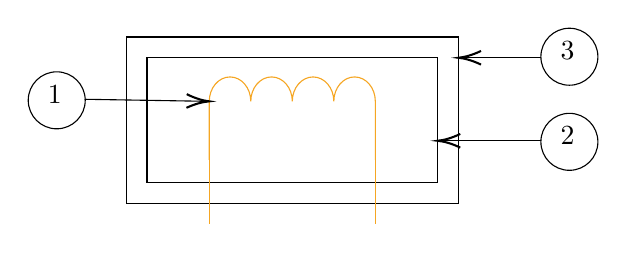
\begin{tikzpicture}[x=0.75pt,y=0.75pt,yscale=-1,xscale=1]
%uncomment if require: \path (0,300); %set diagram left start at 0, and has height of 300
%Shape: Rectangle [id:dp6431615116150586] 
\draw   (120,100) -- (260,100) -- (260,160) -- (120,160) -- cycle ;
%Shape: Rectangle [id:dp21722968746615745] 
\draw   (110,90) -- (270,90) -- (270,170) -- (110,170) -- cycle ;
%Shape: Inductor [id:dp2168804832907768] 
\draw  [color={rgb, 255:red, 245; green, 166; blue, 35 }  ,draw opacity=1 ] (150,149.24) -- (150,121) .. controls (150,114.51) and (154.48,109.24) .. (160,109.24) .. controls (165.52,109.24) and (170,114.51) .. (170,121) .. controls (170,114.51) and (174.48,109.24) .. (180,109.24) .. controls (185.52,109.24) and (190,114.51) .. (190,121) .. controls (190,114.51) and (194.48,109.24) .. (200,109.24) .. controls (205.52,109.24) and (210,114.51) .. (210,121) .. controls (210,114.51) and (214.48,109.24) .. (220,109.24) .. controls (225.52,109.24) and (230,114.51) .. (230,121) -- (230,149.24) ;
%Straight Lines [id:da9190346443391305] 
\draw [color={rgb, 255:red, 245; green, 166; blue, 35 }  ,draw opacity=1 ]   (150,149.24) -- (150,180) ;
%Straight Lines [id:da1556694134502471] 
\draw [color={rgb, 255:red, 245; green, 166; blue, 35 }  ,draw opacity=1 ]   (230,149.24) -- (230,180) ;
%Straight Lines [id:da6906822080495362] 
\draw    (90,120) -- (148,120.97) ;
\draw [shift={(150,121)}, rotate = 180.95] [color={rgb, 255:red, 0; green, 0; blue, 0 }  ][line width=0.75]    (10.93,-3.29) .. controls (6.95,-1.4) and (3.31,-0.3) .. (0,0) .. controls (3.31,0.3) and (6.95,1.4) .. (10.93,3.29)   ;
%Straight Lines [id:da8500651824334423] 
\draw    (310,100) -- (272,100) ;
\draw [shift={(270,100)}, rotate = 360] [color={rgb, 255:red, 0; green, 0; blue, 0 }  ][line width=0.75]    (10.93,-3.29) .. controls (6.95,-1.4) and (3.31,-0.3) .. (0,0) .. controls (3.31,0.3) and (6.95,1.4) .. (10.93,3.29)   ;
%Straight Lines [id:da6409885852889874] 
\draw    (310,140) -- (262,140) ;
\draw [shift={(260,140)}, rotate = 360] [color={rgb, 255:red, 0; green, 0; blue, 0 }  ][line width=0.75]    (10.93,-3.29) .. controls (6.95,-1.4) and (3.31,-0.3) .. (0,0) .. controls (3.31,0.3) and (6.95,1.4) .. (10.93,3.29)   ;

% Text Node
\draw    (76.5, 120.5) circle [x radius= 13.73, y radius= 13.73]   ;
\draw (71,112) node [anchor=north west][inner sep=0.75pt]   [align=left] {1};
% Text Node
\draw    (323.5, 140.5) circle [x radius= 13.73, y radius= 13.73]   ;
\draw (318,132) node [anchor=north west][inner sep=0.75pt]   [align=left] {2};
% Text Node
\draw    (323.5, 99.5) circle [x radius= 13.73, y radius= 13.73]   ;
\draw (318,91) node [anchor=north west][inner sep=0.75pt]   [align=left] {3};
\end{tikzpicture}
\end{figure}


\subsection{Dispositif Différentiel Résiduel}

\subsubsection{Caractéristiques générales}

\begin{definition}[Dispositif Différentiel Résiduel]
Un Dispositif Différentiel Résiduel (DDR) est un appareil de protection chargé d'assurer la protection des personnes contre les défauts d'isolement provoquant potentiellement des contacts indirects (\superref{def:contact_indirect}). Son rôle est de surveiller les fuites de courant d'une installation électrique vers la terre.
\end{definition}

Il convient de bien différencier deux type de DDR :
\begin{description}
\item[Interrupteur différentiel :] protection des personnes contre les contacts indirects dont le symbole est : \\
\begin{center}
\tikzset{every picture/.style={line width=0.75pt}} %set default line width to 0.75pt        
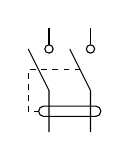
\begin{tikzpicture}[x=0.75pt,y=0.75pt,yscale=-1,xscale=1]
%uncomment if require: \path (0,300); %set diagram left start at 0, and has height of 300
%Straight Lines [id:da2706332247205] 
\draw    (322.5,125) -- (332.5,145) -- (332.5,165) ;
%Shape: Circle [id:dp29153358238009897] 
\draw   (334.5,125) .. controls (334.5,123.9) and (333.6,123) .. (332.5,123) .. controls (331.4,123) and (330.5,123.9) .. (330.5,125) .. controls (330.5,126.1) and (331.4,127) .. (332.5,127) .. controls (333.6,127) and (334.5,126.1) .. (334.5,125) -- cycle ;
%Straight Lines [id:da6197793752064008] 
\draw    (332.5,123) -- (332.5,115) ;
%Straight Lines [id:da23336746577348777] 
\draw    (342.5,125) -- (352.5,145) -- (352.5,165) ;
%Shape: Circle [id:dp8550359924354977] 
\draw   (354.5,125) .. controls (354.5,123.9) and (353.6,123) .. (352.5,123) .. controls (351.4,123) and (350.5,123.9) .. (350.5,125) .. controls (350.5,126.1) and (351.4,127) .. (352.5,127) .. controls (353.6,127) and (354.5,126.1) .. (354.5,125) -- cycle ;
%Straight Lines [id:da05305444358418154] 
\draw    (352.5,123) -- (352.5,115) ;
%Rounded Rect [id:dp05115241565335704] 
\draw   (327.5,155) .. controls (327.5,153.62) and (328.62,152.5) .. (330,152.5) -- (355,152.5) .. controls (356.38,152.5) and (357.5,153.62) .. (357.5,155) -- (357.5,155) .. controls (357.5,156.38) and (356.38,157.5) .. (355,157.5) -- (330,157.5) .. controls (328.62,157.5) and (327.5,156.38) .. (327.5,155) -- cycle ;
%Straight Lines [id:da939318430006016] 
\draw  [dash pattern={on 2pt off 2pt}]  (347.5,135) -- (322.5,135) -- (322.5,155) -- (327.5,155) ;
\end{tikzpicture}
\end{center}
\item[Disjoncteur différentiel :] protection des personnes contre les contacts indirects et protection des circuits contre les surintensités et les court-circuits dont le symbole est : \\
\begin{center}
\tikzset{every picture/.style={line width=0.75pt}} %set default line width to 0.75pt        
\begin{tikzpicture}[x=0.75pt,y=0.75pt,yscale=-1,xscale=1]
%uncomment if require: \path (0,300); %set diagram left start at 0, and has height of 300
%Straight Lines [id:da7942674629541203] 
\draw    (240,80) -- (250,100) -- (250,120) ;
%Straight Lines [id:da02504818626569283] 
\draw    (250,80) -- (250,70) ;
%Straight Lines [id:da5265041115987463] 
\draw    (260,80) -- (270,100) -- (270,120) ;
%Rounded Rect [id:dp7509265725897157] 
\draw   (245,110) .. controls (245,108.62) and (246.12,107.5) .. (247.5,107.5) -- (272.5,107.5) .. controls (273.88,107.5) and (275,108.62) .. (275,110) -- (275,110) .. controls (275,111.38) and (273.88,112.5) .. (272.5,112.5) -- (247.5,112.5) .. controls (246.12,112.5) and (245,111.38) .. (245,110) -- cycle ;
%Straight Lines [id:da683110463277837] 
\draw  [dash pattern={on 2pt off 2pt}]  (265,90) -- (240,90) -- (240,110) -- (245,110) ;
%Straight Lines [id:da9974991339852742] 
\draw    (248,78) -- (252,82) ;
%Straight Lines [id:da7033873514321916] 
\draw    (252,78) -- (248,82) ;
%Straight Lines [id:da03830277666277171] 
\draw    (270,80) -- (270,70) ;
%Straight Lines [id:da28905723063553246] 
\draw    (268,78) -- (272,82) ;
%Straight Lines [id:da007952841582709036] 
\draw    (272,78) -- (268,82) ;
\end{tikzpicture}
\end{center}
\end{description}

\begin{table}[h]
\caption{Valeur du seuil de $I_{\Delta n}$ fonction de $R_{A}$ et $U_{L}$}
\begin{tabularx}{\linewidth}{C i k S C i k S C i k S}
\toprule
\thead{$U_{L}$}	& \multicolumn{2}{c}{\thead{$R_{A}$ (\si{\ohm})}}	& 	{$I_{\Delta n}$ (\si{\ampere})}	& \thead{$U_{L}$}	& \multicolumn{2}{c}{\thead{$R_{A}$ (\si{\ohm})}}	& 	{$I_{\Delta n}$ (\si{\ampere})} & \thead{$U_{L}$}	& \multicolumn{2}{c}{\thead{$R_{A}$ (\si{\ohm})}}	& 	{$I_{\Delta n}$ (\si{\ampere})}	\\
\midrule
\SI{50}{\volt}	& \geq & 1660	&  0,030 		& \SI{25}{\volt}	& \geq & 500	& 	0,030	& \SI{12}{\volt}		& \geq & 400	&  0,030 \\
						& \geq & 166		&  0,300 		& 							& \geq & 83	&  0,300 	& 								& \geq & 40	&  0,300  \\
						& \geq & 100		&  0,500 		& 							& \geq & 50	&  0,500 	& 								& \geq & 24	&  0,500  \\
						& \geq & 16		&  3				& 							& \geq & 8		& 		 3 		& 								& \geq & 4		&  3  \\
\bottomrule
\end{tabularx}
\end{table}

\subsubsection{Marquage normalisé}

Comme tout appareil de protection, le DDR respecte des normes de qualité strictes (Conformité Européenne) et doivent présenter plusieurs marquages réglementaires, ainsi qu'un bouton \og TEST \fg{} pour informer l'installateur et l'utilisateur des caractéristiques du DDR. Cela informe de la conformité de l'appareil de protection.

\begin{center}
\begin{figure}[h]
\caption{Marquage d'un interrupteur différentiel}
\begin{subfigure}[t]{0.49\linewidth}
\subcaption{Vue de dessus}
\begin{annotate}
{\includegraphics[scale=1]{DDR_dessus}}{0.25}
%\helpgrid[gray] 
\node at (-11.8,4.3) {\cstep\label{pas:1}};
\node at (-11.8,2.2) {\cstep\label{pas:2}};
\node at (-11.8,-0.85) {\cstep\label{pas:3}};
\node at (-11.8,-3.85) {\cstep\label{pas:4}};
\node at (11.7,3.4) {\cstep\label{pas:5}};
\node at (11.7,1.1) {\cstep\label{pas:6}};
\node at (11.7,-2.1) {\cstep\label{pas:7}};
\end{annotate} 
\end{subfigure}
\begin{subfigure}[t]{0.49\linewidth}
\subcaption{Vue de dessus}
\begin{annotate}
{\includegraphics[scale=1]{DDR_avant}}{0.25}
%\helpgrid[gray] 
\node at (-11.8,6.7) {\cstep\label{pas:8}};
\node at (-11.8,3.8) {\cstep\label{pas:9}};
\node at (-11.9,-6.85) {\cstep\label{pas:10}};
\node at (11.7,3.85) {\cstep\label{pas:11}};
\node at (11.7,1) {\cstep\label{pas:12}};
\node at (11.7,-2.05) {\cstep\label{pas:13}};
\end{annotate} 
\end{subfigure}
\end{figure}
\end{center}

\begin{minipage}{\linewidth} %usage d'un environnement mini-page pour éviter les décalage au début de la première colonne quand l'élément n'est pas du texte simple
	\begin{multicols}{2} %répartition du texte dans l'environnement en deux colonnes
		\circref{pas:1}norme du produit\\ %légende automatique
		\circref{pas:2}tension assignée $230/400\si{\volt}\sim$\\
		\circref{pas:3}code de production\\
		\circref{pas:4}signe \og Courant assigné de court-circuit \SI{10000}{\ampere} \fg{} en combinaison avec un fusible en amont \\
		\circref{pas:5}pouvoir assigné de coupure \og \SI{1250}{\ampere} \fg{} \\
		\circref{pas:6}signe de sécurité ESTI (équivalent de la norme NF poiur la Suisse \\
		\circref{pas:7}signe \og Flocon de neige \fg{} (utilisation pour une température ambiante jusqu'à \SI{-25}{\degree}) \\
		\columnbreak\\ %passage à la deuxième colonne
		\circref{pas:8}couple de serrage \si{\newton\meter} \\
		\circref{pas:9}désignation du type\\
		\circref{pas:10}schéma des connexions\\
		\circref{pas:11}courant assigné $I_n$ de \SI{40}{\ampere} et calibre du DDR $I_{\Delta n}$\\
		\circref{pas:12}note concernant le test \og à effectuer tous les six mois \fg{}\\
		 \circref{pas:13}type de courant différentiel (type F)
	\end{multicols}
\end{minipage}

\subsubsection{Composante du courant de défaut}

Les DDR peuvent détecter plusieurs composantes du courant de défaut. C'est un paramètre qui peut varier selon le type d'appareil électrique protégé par le DDR.

\begin{xltabular}{\textwidth}{c c X c c }
\caption{Différents types de DDR selon les composantes du courant de défaut}\\
\toprule
\thead{Type}		& \thead{Symbole}		& \thead{Caractéristiques}	& \thead{Forme d'onde}		& \thead{Type de charge} \\
\midrule
\endfirsthead %en-tête de la première page du tableau  
\multicolumn{5}{l}{\small\textit{Page précédente}} \\
\midrule %filet de milieu de tableau
\thead{Type}		& \thead{Symbole}		& \thead{Caractéristiques}	& \thead{Forme d'onde}		& \thead{Type de charge} \\
\midrule
\endhead
\midrule %filet de milieu de tableau
\multicolumn{5}{r}{\small\textit{Page suivante}} \\
\endfoot %pied de page de toutes les pages du tableau
\bottomrule
\endlastfoot %pied de page de la dernièredu tableau
Type AC		& \adjustbox{valign=t}{\includegraphics[height=0.4cm]{type_ac.png}}		& 
\begin{tabitemize}
\item détection des courants alternatifs résiduels 
\item utilisation courante en domestique couvrant la plupart des besoin 
\end{tabitemize}
& & \\
\end{xltabular}


\subsection{Mise à la terre des appareils et structures conductrices}

\subsubsection{Mise à la terre des appareils électriques}

Les appareils de classe d'isolation I doivent être raccordées à des prises 2P + T \Circled{1} au moyen de fiches 2P + T \Circled{2}. Ces prises équipent maintenant tous les logements dont l'installation respecte la norme NF C15-100. Si ces appareils ne présentent pas de fiches, elles sont raccordées au moyen de boitiers d'encastrements appropriés.\\
Sont particulièrement concernés par cette connexion vers la terre les appareils combinant électricité et eau (lave-vaisselle, lave-linge, cafetière\ldots \Circled{3}). Les fuites d'eau peuvent effectivement  provoquer relativement facilement la mise sous tension de la carcasse métallique de l'appareil.

\subsubsection{Liaison équipotentielle}

Pour protéger les biens et les personnes des contacts indirects, en plus de connecter toutes les carcasses métalliques des appareils de classe d'isolation II vers la terre, il convient de connecter toutes les structures métalliques du bâtiment susceptibles d'être en contact avec un individu \emph{et} d'être mise sous tension accidentellement. Sont concernés par la mise à la terre \Circled{4} :
\begin{itemize}
\item tuyauterie (même non conductrice car l'eau y transitant l'est)\,;
\item baignoire et bac de douche (fonte, métal\ldots)\,;
\item charpente métallique\,;
\item autres structures métalliques (pouvant varier selon les exigences de sécurité).
\end{itemize}
Cette connexion, effectuée par un \emph{conducteur de protection} PE \Circled{5} (obligatoirement en jaune-vert), de toutes les structures conductrices et appareils de classe I constitue la \emph{liaison équipotentielle}. Tous ces conducteurs sont connectés sur une \emph{barrette de terre} \Circled{8} dans le Tableau Général Basse Tension (TGBT) et sont séparés de la \emph{prise de terre de l'installation électrique} \Circled{9} par une \emph{barrette de mesure} \Circled{10} (dénommé également \emph{couteau de terre}).\\

Afin d'assurer la meilleure protection possible, les conducteurs de protection doivent présenter une section de câble et des raccordements dimensionnés à même de garantir une résistance de la liaison équipotentielle d'une valeur inférieure à \SI{2}{\ohm}. Cette résistance est contrôlée au moyen d'un \emph{testeur de continuité} spécifique.
\begin{table}[H]
\caption{Section des conducteurs de protection}
\begin{tabularx}{\linewidth}{c X p{5,5cm}}
\toprule
\thead{Schéma}		& \thead{Type de conducteur}		& \thead{Section} \\
\midrule
\Circled{5} 		& Conducteur de protection transitant dans la même canalisation que les phase(s) et neutre		& identique à celle des phase(s) et neutre \\
\addlinespace
	&		Conducteur de protection protégé mécaniquement																	& \SI{2,5}{\square\milli\meter} \\
\addlinespace
	&		Conducteur de protection non protégé mécaniquement															& \SI{4}{\square\milli\meter} \\
\addlinespace
\Circled{6}		&	Conducteur principal de protection																							& \SI{16}{\square\milli\meter} en cuivre isolé \\
\addlinespace
\Circled{7} 		& Conducteur de terre																												& 
\begin{tabdescription}
\item[Selon les caractéristiques :]\hfill
\begin{compactitemize}
\item \SI{16}{\square\milli\meter} en cuivre isolé\,;
\item \SI{25}{\square\milli\meter} en cuivre nu\,;
\item \SI{50}{\square\milli\meter} en aluminium ou en fer.
\end{compactitemize} 
\end{tabdescription}
\\
\bottomrule
\end{tabularx}
\end{table}

%--------------------------------------
%ELECTROTECHNIQUE - SCHEMA DE LIAISON A LA TERRE
%--------------------------------------

%utiliser les environnement \begin{comment} \end{comment} pour mettre en commentaire le préambule une fois la programmation appelée dans le document maître (!ne pas oublier de mettre en commentaire \end{document}!)

\begin{comment}

\documentclass[a4paper, 11pt, twoside, fleqn]{memoir}

\usepackage{AOCDTF}

%--------------------------------------
%CANEVAS
%--------------------------------------

\newcommand\BoxColor{\ifcase\thechapshift blue!30\or brown!30\or pink!30\or cyan!30\or green!30\or teal!30\or purple!30\or red!30\or olive!30\or orange!30\or lime!30\or gray!\or magenta!30\else yellow!30\fi} %définition de la couleur des marqueurs de chapitre

\newcounter{chapshift} %compteur de chapitre du marqueur de chapitre
\addtocounter{chapshift}{-1}
	
\newif\ifFrame %instruction conditionnelle pour les couleurs des pages
\Frametrue

\pagestyle{plain}

% the main command; the mandatory argument sets the color of the vertical box
\newcommand\ChapFrame{%
\AddEverypageHook{%
\ifFrame
\ifthenelse{\isodd{\value{page}}}
  {\backgroundsetup{contents={%
  \begin{tikzpicture}[overlay,remember picture]
  \node[
  	rounded corners=3pt,
    fill=\BoxColor,
    inner sep=0pt,
    rectangle,
    text width=1.5cm,
    text height=5.5cm,
    align=center,
    anchor=north west
  ] 
  at ($ (current page.north west) + (-0cm,-2*\thechapshift cm) $) %nombre négatif = espacement des marqueurs entre les différents chapitres (à régler en fin de rédaction) (4.5cm vaut un espacement équivalement à la hauteur du marqueur, une page peut en contenir 6 avec cet espacement-la mais il est le plus équilibré)
    {\rotatebox{90}{\hspace*{.5cm}%
      \parbox[c][1.2cm][t]{5cm}{%
        \raggedright\textcolor{black}{\sffamily\textbf{\leftmark}}}}};
  \end{tikzpicture}}}
  }
  {\backgroundsetup{contents={%
  \begin{tikzpicture}[overlay,remember picture]
  \node[
  	rounded corners=3pt,
    fill=\BoxColor,
    inner sep=0pt,
    rectangle,
    text width=1.5cm,
    text height=5.5cm,
    align=center,
    anchor=north east
  ] 
  at ($ (current page.north east) + (-0cm,-2*\thechapshift cm) $) %nombre négatif = espacement des marqueurs entre les différents chapitres (à régler en fin de rédaction) (4.5cm vaut un espacement équivalement à la hauteur du marqueur, une page peut en contenir 6 avec cet espacement-la mais il est le plus équilibré)
    {\rotatebox{90}{\hspace*{.5cm}%
      \parbox[c][1.2cm][t]{5cm}{%
        \raggedright\textcolor{black}{\sffamily\textbf{\leftmark}}}}};
  \end{tikzpicture}}}%
  }
  \BgMaterial%
  \fi%
}%
  \stepcounter{chapshift}
}

\renewcommand\chaptermark[1]{\markboth{\thechapter.~#1}{}} %redéfinition du marqueur de chapitre pour ne contenir que le titre du chapitre %à personnaliser selon le nombre de chapitre dans le cours

%--------------------------------------
%corps du document
%--------------------------------------

\begin{document} %corps du document
	\openleft %début de chapitre à gauche

\end{comment}


\begin{figure}
\caption{Liaison équipotentielle}


\tikzset{every picture/.style={line width=0.75pt}} %set default line width to 0.75pt        

\begin{tikzpicture}[x=0.75pt,y=0.75pt,yscale=-1,xscale=1]
%uncomment if require: \path (0,484); %set diagram left start at 0, and has height of 484

%Shape: Rectangle [id:dp12779471624214456] 
\draw  [color={rgb, 255:red, 245; green, 108; blue, 35 }  ,draw opacity=1 ][fill={rgb, 255:red, 245; green, 108; blue, 35 }  ,fill opacity=1 ] (203.5,349.9) -- (340,349.9) -- (340,365) -- (203.5,365) -- cycle ;
%Shape: Circle [id:dp3978776166680479] 
\draw  [color={rgb, 255:red, 245; green, 166; blue, 35 }  ,draw opacity=1 ][fill={rgb, 255:red, 245; green, 166; blue, 35 }  ,fill opacity=1 ] (211,357.5) .. controls (211,355.57) and (212.57,354) .. (214.5,354) .. controls (216.43,354) and (218,355.57) .. (218,357.5) .. controls (218,359.43) and (216.43,361) .. (214.5,361) .. controls (212.57,361) and (211,359.43) .. (211,357.5) -- cycle ;
%Shape: Rectangle [id:dp5513162261841694] 
\draw  [color={rgb, 255:red, 245; green, 94; blue, 35 }  ,draw opacity=1 ][fill={rgb, 255:red, 245; green, 166; blue, 35 }  ,fill opacity=1 ] (215.91,355.38) -- (216.62,356.09) -- (213.09,359.62) -- (212.38,358.91) -- cycle ;

%Shape: Circle [id:dp990223085537162] 
\draw  [color={rgb, 255:red, 245; green, 166; blue, 35 }  ,draw opacity=1 ][fill={rgb, 255:red, 245; green, 166; blue, 35 }  ,fill opacity=1 ] (221,357.5) .. controls (221,355.57) and (222.57,354) .. (224.5,354) .. controls (226.43,354) and (228,355.57) .. (228,357.5) .. controls (228,359.43) and (226.43,361) .. (224.5,361) .. controls (222.57,361) and (221,359.43) .. (221,357.5) -- cycle ;
%Shape: Rectangle [id:dp7901194427174768] 
\draw  [color={rgb, 255:red, 245; green, 94; blue, 35 }  ,draw opacity=1 ][fill={rgb, 255:red, 245; green, 166; blue, 35 }  ,fill opacity=1 ] (225.91,355.38) -- (226.62,356.09) -- (223.09,359.62) -- (222.38,358.91) -- cycle ;

%Shape: Circle [id:dp23561107154810057] 
\draw  [color={rgb, 255:red, 245; green, 166; blue, 35 }  ,draw opacity=1 ][fill={rgb, 255:red, 245; green, 166; blue, 35 }  ,fill opacity=1 ] (231,357.5) .. controls (231,355.57) and (232.57,354) .. (234.5,354) .. controls (236.43,354) and (238,355.57) .. (238,357.5) .. controls (238,359.43) and (236.43,361) .. (234.5,361) .. controls (232.57,361) and (231,359.43) .. (231,357.5) -- cycle ;
%Shape: Rectangle [id:dp2645964583580035] 
\draw  [color={rgb, 255:red, 245; green, 94; blue, 35 }  ,draw opacity=1 ][fill={rgb, 255:red, 245; green, 166; blue, 35 }  ,fill opacity=1 ] (235.91,355.38) -- (236.62,356.09) -- (233.09,359.62) -- (232.38,358.91) -- cycle ;

%Shape: Circle [id:dp004074096804411842] 
\draw  [color={rgb, 255:red, 245; green, 166; blue, 35 }  ,draw opacity=1 ][fill={rgb, 255:red, 245; green, 166; blue, 35 }  ,fill opacity=1 ] (241,357.5) .. controls (241,355.57) and (242.57,354) .. (244.5,354) .. controls (246.43,354) and (248,355.57) .. (248,357.5) .. controls (248,359.43) and (246.43,361) .. (244.5,361) .. controls (242.57,361) and (241,359.43) .. (241,357.5) -- cycle ;
%Shape: Rectangle [id:dp15563792683915179] 
\draw  [color={rgb, 255:red, 245; green, 94; blue, 35 }  ,draw opacity=1 ][fill={rgb, 255:red, 245; green, 166; blue, 35 }  ,fill opacity=1 ] (245.91,355.38) -- (246.62,356.09) -- (243.09,359.62) -- (242.38,358.91) -- cycle ;

%Shape: Circle [id:dp42723031236585807] 
\draw  [color={rgb, 255:red, 245; green, 166; blue, 35 }  ,draw opacity=1 ][fill={rgb, 255:red, 245; green, 166; blue, 35 }  ,fill opacity=1 ] (251,357.5) .. controls (251,355.57) and (252.57,354) .. (254.5,354) .. controls (256.43,354) and (258,355.57) .. (258,357.5) .. controls (258,359.43) and (256.43,361) .. (254.5,361) .. controls (252.57,361) and (251,359.43) .. (251,357.5) -- cycle ;
%Shape: Rectangle [id:dp23601803414152545] 
\draw  [color={rgb, 255:red, 245; green, 94; blue, 35 }  ,draw opacity=1 ][fill={rgb, 255:red, 245; green, 166; blue, 35 }  ,fill opacity=1 ] (255.91,355.38) -- (256.62,356.09) -- (253.09,359.62) -- (252.38,358.91) -- cycle ;

%Shape: Circle [id:dp21722774235746978] 
\draw  [color={rgb, 255:red, 245; green, 166; blue, 35 }  ,draw opacity=1 ][fill={rgb, 255:red, 245; green, 166; blue, 35 }  ,fill opacity=1 ] (261,357.5) .. controls (261,355.57) and (262.57,354) .. (264.5,354) .. controls (266.43,354) and (268,355.57) .. (268,357.5) .. controls (268,359.43) and (266.43,361) .. (264.5,361) .. controls (262.57,361) and (261,359.43) .. (261,357.5) -- cycle ;
%Shape: Rectangle [id:dp3473865244123996] 
\draw  [color={rgb, 255:red, 245; green, 94; blue, 35 }  ,draw opacity=1 ][fill={rgb, 255:red, 245; green, 166; blue, 35 }  ,fill opacity=1 ] (265.91,355.38) -- (266.62,356.09) -- (263.09,359.62) -- (262.38,358.91) -- cycle ;

%Shape: Circle [id:dp43806185211532767] 
\draw  [color={rgb, 255:red, 245; green, 166; blue, 35 }  ,draw opacity=1 ][fill={rgb, 255:red, 245; green, 166; blue, 35 }  ,fill opacity=1 ] (271,357.5) .. controls (271,355.57) and (272.57,354) .. (274.5,354) .. controls (276.43,354) and (278,355.57) .. (278,357.5) .. controls (278,359.43) and (276.43,361) .. (274.5,361) .. controls (272.57,361) and (271,359.43) .. (271,357.5) -- cycle ;
%Shape: Rectangle [id:dp47605810022702744] 
\draw  [color={rgb, 255:red, 245; green, 94; blue, 35 }  ,draw opacity=1 ][fill={rgb, 255:red, 245; green, 166; blue, 35 }  ,fill opacity=1 ] (275.91,355.38) -- (276.62,356.09) -- (273.09,359.62) -- (272.38,358.91) -- cycle ;

%Shape: Circle [id:dp12453339823990162] 
\draw  [color={rgb, 255:red, 245; green, 166; blue, 35 }  ,draw opacity=1 ][fill={rgb, 255:red, 245; green, 166; blue, 35 }  ,fill opacity=1 ] (281,357.5) .. controls (281,355.57) and (282.57,354) .. (284.5,354) .. controls (286.43,354) and (288,355.57) .. (288,357.5) .. controls (288,359.43) and (286.43,361) .. (284.5,361) .. controls (282.57,361) and (281,359.43) .. (281,357.5) -- cycle ;
%Shape: Rectangle [id:dp6051367753026781] 
\draw  [color={rgb, 255:red, 245; green, 94; blue, 35 }  ,draw opacity=1 ][fill={rgb, 255:red, 245; green, 166; blue, 35 }  ,fill opacity=1 ] (285.91,355.38) -- (286.62,356.09) -- (283.09,359.62) -- (282.38,358.91) -- cycle ;

%Shape: Circle [id:dp7759537392826514] 
\draw  [color={rgb, 255:red, 245; green, 166; blue, 35 }  ,draw opacity=1 ][fill={rgb, 255:red, 245; green, 166; blue, 35 }  ,fill opacity=1 ] (291,357.5) .. controls (291,355.57) and (292.57,354) .. (294.5,354) .. controls (296.43,354) and (298,355.57) .. (298,357.5) .. controls (298,359.43) and (296.43,361) .. (294.5,361) .. controls (292.57,361) and (291,359.43) .. (291,357.5) -- cycle ;
%Shape: Rectangle [id:dp917105554714615] 
\draw  [color={rgb, 255:red, 245; green, 94; blue, 35 }  ,draw opacity=1 ][fill={rgb, 255:red, 245; green, 166; blue, 35 }  ,fill opacity=1 ] (295.91,355.38) -- (296.62,356.09) -- (293.09,359.62) -- (292.38,358.91) -- cycle ;

%Shape: Circle [id:dp02780975411771036] 
\draw  [color={rgb, 255:red, 245; green, 166; blue, 35 }  ,draw opacity=1 ][fill={rgb, 255:red, 245; green, 166; blue, 35 }  ,fill opacity=1 ] (301,357.5) .. controls (301,355.57) and (302.57,354) .. (304.5,354) .. controls (306.43,354) and (308,355.57) .. (308,357.5) .. controls (308,359.43) and (306.43,361) .. (304.5,361) .. controls (302.57,361) and (301,359.43) .. (301,357.5) -- cycle ;
%Shape: Rectangle [id:dp33128134488839245] 
\draw  [color={rgb, 255:red, 245; green, 94; blue, 35 }  ,draw opacity=1 ][fill={rgb, 255:red, 245; green, 166; blue, 35 }  ,fill opacity=1 ] (305.91,355.38) -- (306.62,356.09) -- (303.09,359.62) -- (302.38,358.91) -- cycle ;

%Shape: Circle [id:dp24766499702501743] 
\draw  [color={rgb, 255:red, 245; green, 166; blue, 35 }  ,draw opacity=1 ][fill={rgb, 255:red, 245; green, 166; blue, 35 }  ,fill opacity=1 ] (311,357.5) .. controls (311,355.57) and (312.57,354) .. (314.5,354) .. controls (316.43,354) and (318,355.57) .. (318,357.5) .. controls (318,359.43) and (316.43,361) .. (314.5,361) .. controls (312.57,361) and (311,359.43) .. (311,357.5) -- cycle ;
%Shape: Rectangle [id:dp9353732861352104] 
\draw  [color={rgb, 255:red, 245; green, 94; blue, 35 }  ,draw opacity=1 ][fill={rgb, 255:red, 245; green, 166; blue, 35 }  ,fill opacity=1 ] (315.91,355.38) -- (316.62,356.09) -- (313.09,359.62) -- (312.38,358.91) -- cycle ;

%Shape: Circle [id:dp37341465274388497] 
\draw  [color={rgb, 255:red, 245; green, 166; blue, 35 }  ,draw opacity=1 ][fill={rgb, 255:red, 245; green, 166; blue, 35 }  ,fill opacity=1 ] (324,357) .. controls (324,353.69) and (326.69,351) .. (330,351) .. controls (333.31,351) and (336,353.69) .. (336,357) .. controls (336,360.31) and (333.31,363) .. (330,363) .. controls (326.69,363) and (324,360.31) .. (324,357) -- cycle ;
%Shape: Rectangle [id:dp9630557822680567] 
\draw  [color={rgb, 255:red, 245; green, 94; blue, 35 }  ,draw opacity=1 ][fill={rgb, 255:red, 245; green, 94; blue, 35 }  ,fill opacity=1 ] (332.42,353.36) -- (333.64,354.58) -- (327.58,360.64) -- (326.36,359.42) -- cycle ;

%Straight Lines [id:da24513459081521916] 
\draw [color={rgb, 255:red, 126; green, 211; blue, 33 }  ,draw opacity=1 ]   (20,220) -- (20,300) -- (214.66,300) -- (214.5,354) ;
%Shape: Rectangle [id:dp9788722615305224] 
\draw  [color={rgb, 255:red, 0; green, 0; blue, 0 }  ,draw opacity=1 ][fill={rgb, 255:red, 0; green, 0; blue, 0 }  ,fill opacity=1 ] (295,215) -- (285,215) -- (285,190) -- (295,190) -- cycle ;
%Shape: Arc [id:dp4625855025240825] 
\draw  [draw opacity=0] (299.97,207.41) .. controls (299.99,207.73) and (300,208.05) .. (300,208.38) .. controls (300,214.8) and (295.52,220) .. (290,220) .. controls (284.48,220) and (280,214.8) .. (280,208.38) .. controls (280,208.05) and (280.01,207.73) .. (280.03,207.41) -- (290,208.38) -- cycle ; \draw   (299.97,207.41) .. controls (299.99,207.73) and (300,208.05) .. (300,208.38) .. controls (300,214.8) and (295.52,220) .. (290,220) .. controls (284.48,220) and (280,214.8) .. (280,208.38) .. controls (280,208.05) and (280.01,207.73) .. (280.03,207.41) ;
%Straight Lines [id:da92206048726559] 
\draw    (280.03,207.41) -- (280,200) ;
%Straight Lines [id:da9786762971174932] 
\draw    (300,200) -- (299.97,207.41) ;
%Shape: Rectangle [id:dp6334689518753208] 
\draw  [color={rgb, 255:red, 0; green, 0; blue, 0 }  ,draw opacity=1 ][fill={rgb, 255:red, 0; green, 0; blue, 0 }  ,fill opacity=1 ] (250,215) -- (240,215) -- (240,190) -- (250,190) -- cycle ;
%Shape: Arc [id:dp9577852186178959] 
\draw  [draw opacity=0] (254.97,207.41) .. controls (254.99,207.73) and (255,208.05) .. (255,208.38) .. controls (255,214.8) and (250.52,220) .. (245,220) .. controls (239.48,220) and (235,214.8) .. (235,208.38) .. controls (235,208.05) and (235.01,207.73) .. (235.03,207.41) -- (245,208.38) -- cycle ; \draw   (254.97,207.41) .. controls (254.99,207.73) and (255,208.05) .. (255,208.38) .. controls (255,214.8) and (250.52,220) .. (245,220) .. controls (239.48,220) and (235,214.8) .. (235,208.38) .. controls (235,208.05) and (235.01,207.73) .. (235.03,207.41) ;
%Straight Lines [id:da19713391919878898] 
\draw    (235.03,207.41) -- (235,200) ;
%Straight Lines [id:da9861246929342143] 
\draw    (255,200) -- (254.97,207.41) ;
%Shape: Rectangle [id:dp6473840888935389] 
\draw  [color={rgb, 255:red, 0; green, 0; blue, 0 }  ,draw opacity=1 ][fill={rgb, 255:red, 0; green, 0; blue, 0 }  ,fill opacity=1 ] (205,215) -- (195,215) -- (195,190) -- (205,190) -- cycle ;
%Shape: Arc [id:dp2266294248777938] 
\draw  [draw opacity=0] (209.97,207.41) .. controls (209.99,207.73) and (210,208.05) .. (210,208.38) .. controls (210,214.8) and (205.52,220) .. (200,220) .. controls (194.48,220) and (190,214.8) .. (190,208.38) .. controls (190,208.05) and (190.01,207.73) .. (190.03,207.41) -- (200,208.38) -- cycle ; \draw   (209.97,207.41) .. controls (209.99,207.73) and (210,208.05) .. (210,208.38) .. controls (210,214.8) and (205.52,220) .. (200,220) .. controls (194.48,220) and (190,214.8) .. (190,208.38) .. controls (190,208.05) and (190.01,207.73) .. (190.03,207.41) ;
%Straight Lines [id:da47884159630385204] 
\draw    (190.03,207.41) -- (190,200) ;
%Straight Lines [id:da2601506793354168] 
\draw    (210,200) -- (209.97,207.41) ;
%Shape: Rectangle [id:dp8526724245011726] 
\draw  [color={rgb, 255:red, 0; green, 0; blue, 0 }  ,draw opacity=1 ][fill={rgb, 255:red, 0; green, 0; blue, 0 }  ,fill opacity=1 ] (160,215) -- (150,215) -- (150,190) -- (160,190) -- cycle ;
%Shape: Arc [id:dp5006087169417276] 
\draw  [draw opacity=0] (164.97,207.41) .. controls (164.99,207.73) and (165,208.05) .. (165,208.38) .. controls (165,214.8) and (160.52,220) .. (155,220) .. controls (149.48,220) and (145,214.8) .. (145,208.38) .. controls (145,208.05) and (145.01,207.73) .. (145.03,207.41) -- (155,208.38) -- cycle ; \draw   (164.97,207.41) .. controls (164.99,207.73) and (165,208.05) .. (165,208.38) .. controls (165,214.8) and (160.52,220) .. (155,220) .. controls (149.48,220) and (145,214.8) .. (145,208.38) .. controls (145,208.05) and (145.01,207.73) .. (145.03,207.41) ;
%Straight Lines [id:da3667472614970224] 
\draw    (145.03,207.41) -- (145,200) ;
%Straight Lines [id:da3839581039374238] 
\draw    (165,200) -- (164.97,207.41) ;
%Shape: Rectangle [id:dp9963357918533537] 
\draw  [color={rgb, 255:red, 0; green, 0; blue, 0 }  ,draw opacity=1 ][fill={rgb, 255:red, 0; green, 0; blue, 0 }  ,fill opacity=1 ] (115,215) -- (105,215) -- (105,190) -- (115,190) -- cycle ;
%Shape: Arc [id:dp5881658615710518] 
\draw  [draw opacity=0] (119.97,207.41) .. controls (119.99,207.73) and (120,208.05) .. (120,208.38) .. controls (120,214.8) and (115.52,220) .. (110,220) .. controls (104.48,220) and (100,214.8) .. (100,208.38) .. controls (100,208.05) and (100.01,207.73) .. (100.03,207.41) -- (110,208.38) -- cycle ; \draw   (119.97,207.41) .. controls (119.99,207.73) and (120,208.05) .. (120,208.38) .. controls (120,214.8) and (115.52,220) .. (110,220) .. controls (104.48,220) and (100,214.8) .. (100,208.38) .. controls (100,208.05) and (100.01,207.73) .. (100.03,207.41) ;
%Straight Lines [id:da007034621642069916] 
\draw    (100.03,207.41) -- (100,200) ;
%Straight Lines [id:da5445225240782603] 
\draw    (120,200) -- (119.97,207.41) ;
%Shape: Rectangle [id:dp5236717723610569] 
\draw  [color={rgb, 255:red, 0; green, 0; blue, 0 }  ,draw opacity=1 ][fill={rgb, 255:red, 0; green, 0; blue, 0 }  ,fill opacity=1 ] (70,215) -- (60,215) -- (60,190) -- (70,190) -- cycle ;
%Shape: Arc [id:dp9806786756050666] 
\draw  [draw opacity=0] (74.97,207.41) .. controls (74.99,207.73) and (75,208.05) .. (75,208.38) .. controls (75,214.8) and (70.52,220) .. (65,220) .. controls (59.48,220) and (55,214.8) .. (55,208.38) .. controls (55,208.05) and (55.01,207.73) .. (55.03,207.41) -- (65,208.38) -- cycle ; \draw   (74.97,207.41) .. controls (74.99,207.73) and (75,208.05) .. (75,208.38) .. controls (75,214.8) and (70.52,220) .. (65,220) .. controls (59.48,220) and (55,214.8) .. (55,208.38) .. controls (55,208.05) and (55.01,207.73) .. (55.03,207.41) ;
%Shape: Rectangle [id:dp5529771895587449] 
\draw  [color={rgb, 255:red, 0; green, 0; blue, 0 }  ,draw opacity=1 ][fill={rgb, 255:red, 0; green, 0; blue, 0 }  ,fill opacity=1 ] (25,215) -- (15,215) -- (15,190) -- (25,190) -- cycle ;
%Shape: Arc [id:dp35004084572456895] 
\draw  [draw opacity=0] (29.97,207.41) .. controls (29.99,207.73) and (30,208.05) .. (30,208.38) .. controls (30,214.8) and (25.52,220) .. (20,220) .. controls (14.48,220) and (10,214.8) .. (10,208.38) .. controls (10,208.05) and (10.01,207.73) .. (10.03,207.41) -- (20,208.38) -- cycle ; \draw   (29.97,207.41) .. controls (29.99,207.73) and (30,208.05) .. (30,208.38) .. controls (30,214.8) and (25.52,220) .. (20,220) .. controls (14.48,220) and (10,214.8) .. (10,208.38) .. controls (10,208.05) and (10.01,207.73) .. (10.03,207.41) ;
%Straight Lines [id:da7740985330227098] 
\draw    (55.03,207.41) -- (55,200) ;
%Straight Lines [id:da874253942275487] 
\draw    (75,200) -- (74.97,207.41) ;

%Straight Lines [id:da0436588817564304] 
\draw    (10.03,210) -- (10,202.59) ;
%Straight Lines [id:da45394004993381587] 
\draw    (30,202.59) -- (29.97,210) ;
%Straight Lines [id:da4596588122450417] 
\draw [color={rgb, 255:red, 248; green, 231; blue, 28 }  ,draw opacity=1 ] [dash pattern={on 4.5pt off 4.5pt}]  (20,220) -- (20,300) -- (214.66,300) -- (214.5,354) ;
%Straight Lines [id:da7477140703123141] 
\draw [color={rgb, 255:red, 126; green, 211; blue, 33 }  ,draw opacity=1 ]   (35,35) -- (20,35) -- (20,190) ;
%Straight Lines [id:da3286874762261832] 
\draw [color={rgb, 255:red, 248; green, 231; blue, 28 }  ,draw opacity=1 ] [dash pattern={on 4.5pt off 4.5pt}]  (38,35) -- (20,35) -- (20,190) ;
\draw [shift={(40,35)}, rotate = 180] [color={rgb, 255:red, 248; green, 231; blue, 28 }  ,draw opacity=1 ][line width=0.75]    (10.93,-3.29) .. controls (6.95,-1.4) and (3.31,-0.3) .. (0,0) .. controls (3.31,0.3) and (6.95,1.4) .. (10.93,3.29)   ;

%Straight Lines [id:da4598837213780632] 
\draw [color={rgb, 255:red, 126; green, 211; blue, 33 }  ,draw opacity=1 ]   (35,45) -- (20,45) ;
%Straight Lines [id:da839734818655239] 
\draw [color={rgb, 255:red, 248; green, 231; blue, 28 }  ,draw opacity=1 ] [dash pattern={on 4.5pt off 4.5pt}]  (38,45) -- (20,45) ;
\draw [shift={(40,45)}, rotate = 180] [color={rgb, 255:red, 248; green, 231; blue, 28 }  ,draw opacity=1 ][line width=0.75]    (10.93,-3.29) .. controls (6.95,-1.4) and (3.31,-0.3) .. (0,0) .. controls (3.31,0.3) and (6.95,1.4) .. (10.93,3.29)   ;

%Straight Lines [id:da09587209918948914] 
\draw [color={rgb, 255:red, 126; green, 211; blue, 33 }  ,draw opacity=1 ]   (35,55) -- (20,55) ;
%Straight Lines [id:da9944741609170024] 
\draw [color={rgb, 255:red, 248; green, 231; blue, 28 }  ,draw opacity=1 ] [dash pattern={on 4.5pt off 4.5pt}]  (38,55) -- (20,55) ;
\draw [shift={(40,55)}, rotate = 180] [color={rgb, 255:red, 248; green, 231; blue, 28 }  ,draw opacity=1 ][line width=0.75]    (10.93,-3.29) .. controls (6.95,-1.4) and (3.31,-0.3) .. (0,0) .. controls (3.31,0.3) and (6.95,1.4) .. (10.93,3.29)   ;

%Straight Lines [id:da7884693135725294] 
\draw [color={rgb, 255:red, 126; green, 211; blue, 33 }  ,draw opacity=1 ]   (35,65) -- (20,65) ;
%Straight Lines [id:da239241815637814] 
\draw [color={rgb, 255:red, 248; green, 231; blue, 28 }  ,draw opacity=1 ] [dash pattern={on 4.5pt off 4.5pt}]  (38,65) -- (20,65) ;
\draw [shift={(40,65)}, rotate = 180] [color={rgb, 255:red, 248; green, 231; blue, 28 }  ,draw opacity=1 ][line width=0.75]    (10.93,-3.29) .. controls (6.95,-1.4) and (3.31,-0.3) .. (0,0) .. controls (3.31,0.3) and (6.95,1.4) .. (10.93,3.29)   ;

%Straight Lines [id:da8880878687374321] 
\draw [color={rgb, 255:red, 126; green, 211; blue, 33 }  ,draw opacity=1 ]   (35,75) -- (20,75) ;
%Straight Lines [id:da43421080173788573] 
\draw [color={rgb, 255:red, 248; green, 231; blue, 28 }  ,draw opacity=1 ] [dash pattern={on 4.5pt off 4.5pt}]  (38,75) -- (20,75) ;
\draw [shift={(40,75)}, rotate = 180] [color={rgb, 255:red, 248; green, 231; blue, 28 }  ,draw opacity=1 ][line width=0.75]    (10.93,-3.29) .. controls (6.95,-1.4) and (3.31,-0.3) .. (0,0) .. controls (3.31,0.3) and (6.95,1.4) .. (10.93,3.29)   ;

%Straight Lines [id:da4265288409692696] 
\draw [color={rgb, 255:red, 126; green, 211; blue, 33 }  ,draw opacity=1 ]   (35,85) -- (20,85) ;
%Straight Lines [id:da09693100530986232] 
\draw [color={rgb, 255:red, 248; green, 231; blue, 28 }  ,draw opacity=1 ] [dash pattern={on 4.5pt off 4.5pt}]  (38,85) -- (20,85) ;
\draw [shift={(40,85)}, rotate = 180] [color={rgb, 255:red, 248; green, 231; blue, 28 }  ,draw opacity=1 ][line width=0.75]    (10.93,-3.29) .. controls (6.95,-1.4) and (3.31,-0.3) .. (0,0) .. controls (3.31,0.3) and (6.95,1.4) .. (10.93,3.29)   ;

%Straight Lines [id:da18824193936949507] 
\draw [color={rgb, 255:red, 126; green, 211; blue, 33 }  ,draw opacity=1 ]   (35,95) -- (20,95) ;
%Straight Lines [id:da8037918831525122] 
\draw [color={rgb, 255:red, 248; green, 231; blue, 28 }  ,draw opacity=1 ] [dash pattern={on 4.5pt off 4.5pt}]  (38,95) -- (20,95) ;
\draw [shift={(40,95)}, rotate = 180] [color={rgb, 255:red, 248; green, 231; blue, 28 }  ,draw opacity=1 ][line width=0.75]    (10.93,-3.29) .. controls (6.95,-1.4) and (3.31,-0.3) .. (0,0) .. controls (3.31,0.3) and (6.95,1.4) .. (10.93,3.29)   ;

%Straight Lines [id:da7880540826459623] 
\draw [color={rgb, 255:red, 126; green, 211; blue, 33 }  ,draw opacity=1 ]   (65,220) -- (65,290) -- (225,290) -- (225.5,354) ;
%Straight Lines [id:da8587552191330365] 
\draw [color={rgb, 255:red, 248; green, 231; blue, 28 }  ,draw opacity=1 ] [dash pattern={on 4.5pt off 4.5pt}]  (65,220) -- (65,290) -- (159.78,290) -- (225,290) -- (225.5,354) ;
%Straight Lines [id:da6477628826976815] 
\draw [color={rgb, 255:red, 126; green, 211; blue, 33 }  ,draw opacity=1 ]   (65,155) -- (65,155) -- (65,190) ;
%Straight Lines [id:da2838867143416234] 
\draw [color={rgb, 255:red, 248; green, 231; blue, 28 }  ,draw opacity=1 ] [dash pattern={on 4.5pt off 4.5pt}]  (65,155) -- (65,190) ;
%Shape: Rectangle [id:dp04022794256338735] 
\draw   (135,110) -- (175,110) -- (175,155) -- (135,155) -- cycle ;
%Shape: Circle [id:dp7114048760384077] 
\draw  [color={rgb, 255:red, 155; green, 155; blue, 155 }  ,draw opacity=1 ][fill={rgb, 255:red, 80; green, 227; blue, 194 }  ,fill opacity=1 ][line width=3]  (143,137.5) .. controls (143,130.87) and (148.37,125.5) .. (155,125.5) .. controls (161.63,125.5) and (167,130.87) .. (167,137.5) .. controls (167,144.13) and (161.63,149.5) .. (155,149.5) .. controls (148.37,149.5) and (143,144.13) .. (143,137.5) -- cycle ;
%Shape: Rectangle [id:dp24112973693492956] 
\draw  [color={rgb, 255:red, 74; green, 74; blue, 74 }  ,draw opacity=1 ][fill={rgb, 255:red, 74; green, 74; blue, 74 }  ,fill opacity=1 ] (164.5,134.92) -- (169.5,134.92) -- (169.5,140.08) -- (164.5,140.08) -- cycle ;
%Shape: Rectangle [id:dp6934540976609278] 
\draw   (135,110) -- (175,110) -- (175,120) -- (135,120) -- cycle ;
%Shape: Rectangle [id:dp676606923437384] 
\draw  [color={rgb, 255:red, 0; green, 0; blue, 0 }  ,draw opacity=1 ][fill={rgb, 255:red, 208; green, 2; blue, 27 }  ,fill opacity=1 ] (165,110) -- (175,110) -- (175,115) -- (165,115) -- cycle ;
%Shape: Circle [id:dp51451854322091] 
\draw   (162,112.5) .. controls (162,111.95) and (161.55,111.5) .. (161,111.5) .. controls (160.45,111.5) and (160,111.95) .. (160,112.5) .. controls (160,113.05) and (160.45,113.5) .. (161,113.5) .. controls (161.55,113.5) and (162,113.05) .. (162,112.5) -- cycle ;
%Shape: Circle [id:dp08699031717190142] 
\draw   (158,112.5) .. controls (158,111.95) and (157.55,111.5) .. (157,111.5) .. controls (156.45,111.5) and (156,111.95) .. (156,112.5) .. controls (156,113.05) and (156.45,113.5) .. (157,113.5) .. controls (157.55,113.5) and (158,113.05) .. (158,112.5) -- cycle ;
%Shape: Circle [id:dp7550083289144691] 
\draw   (142,114) .. controls (142,112.9) and (141.1,112) .. (140,112) .. controls (138.9,112) and (138,112.9) .. (138,114) .. controls (138,115.1) and (138.9,116) .. (140,116) .. controls (141.1,116) and (142,115.1) .. (142,114) -- cycle ;

%Straight Lines [id:da2873836893966434] 
\draw [color={rgb, 255:red, 126; green, 211; blue, 33 }  ,draw opacity=1 ]   (110,220) -- (110,280) -- (235,280) -- (235.5,354) ;
%Straight Lines [id:da47952347057463585] 
\draw [color={rgb, 255:red, 248; green, 231; blue, 28 }  ,draw opacity=1 ] [dash pattern={on 4.5pt off 4.5pt}]  (110,220) -- (110,280) -- (205,280) -- (235,280) -- (235.5,354) ;
%Straight Lines [id:da2931604104926897] 
\draw [color={rgb, 255:red, 126; green, 211; blue, 33 }  ,draw opacity=1 ]   (110,155) -- (110,155) -- (110,190) ;
%Straight Lines [id:da9190520977970411] 
\draw [color={rgb, 255:red, 248; green, 231; blue, 28 }  ,draw opacity=1 ] [dash pattern={on 4.5pt off 4.5pt}]  (110,155) -- (110,175.64) -- (110,190) ;
%Shape: Rectangle [id:dp33680640738780976] 
\draw   (90,110) -- (130,110) -- (130,155) -- (90,155) -- cycle ;
%Shape: Rectangle [id:dp16425594232501783] 
\draw   (90,110) -- (130,110) -- (130,120) -- (90,120) -- cycle ;
%Shape: Rectangle [id:dp7513935562834199] 
\draw  [color={rgb, 255:red, 0; green, 0; blue, 0 }  ,draw opacity=1 ][fill={rgb, 255:red, 208; green, 2; blue, 27 }  ,fill opacity=1 ] (120,110) -- (130,110) -- (130,115) -- (120,115) -- cycle ;
%Shape: Circle [id:dp4812835434110275] 
\draw   (117,112.5) .. controls (117,111.95) and (116.55,111.5) .. (116,111.5) .. controls (115.45,111.5) and (115,111.95) .. (115,112.5) .. controls (115,113.05) and (115.45,113.5) .. (116,113.5) .. controls (116.55,113.5) and (117,113.05) .. (117,112.5) -- cycle ;
%Shape: Circle [id:dp7330317480363121] 
\draw   (113,112.5) .. controls (113,111.95) and (112.55,111.5) .. (112,111.5) .. controls (111.45,111.5) and (111,111.95) .. (111,112.5) .. controls (111,113.05) and (111.45,113.5) .. (112,113.5) .. controls (112.55,113.5) and (113,113.05) .. (113,112.5) -- cycle ;
%Shape: Circle [id:dp09069500263645891] 
\draw   (97,114) .. controls (97,112.9) and (96.1,112) .. (95,112) .. controls (93.9,112) and (93,112.9) .. (93,114) .. controls (93,115.1) and (93.9,116) .. (95,116) .. controls (96.1,116) and (97,115.1) .. (97,114) -- cycle ;
%Shape: Arc [id:dp36695335781226857] 
\draw  [draw opacity=0] (115,129.84) .. controls (115,129.89) and (115,129.95) .. (115,130) .. controls (115,135.52) and (112.76,140) .. (110,140) .. controls (107.24,140) and (105,135.52) .. (105,130) .. controls (105,129.95) and (105,129.9) .. (105,129.86) -- (110,130) -- cycle ; \draw   (115,129.84) .. controls (115,129.89) and (115,129.95) .. (115,130) .. controls (115,135.52) and (112.76,140) .. (110,140) .. controls (107.24,140) and (105,135.52) .. (105,130) .. controls (105,129.95) and (105,129.9) .. (105,129.86) ;
%Straight Lines [id:da1933122164482982] 
\draw    (110,140) -- (110,150) ;

%Straight Lines [id:da9412467122648331] 
\draw [color={rgb, 255:red, 126; green, 211; blue, 33 }  ,draw opacity=1 ]   (155,220) -- (155,270) -- (245,270) -- (245.5,354) ;
%Straight Lines [id:da04456583562306149] 
\draw [color={rgb, 255:red, 248; green, 231; blue, 28 }  ,draw opacity=1 ] [dash pattern={on 4.5pt off 4.5pt}]  (155,220) -- (155,270) -- (245,270) -- (245,270) -- (245.5,354) ;
%Straight Lines [id:da9382576778304276] 
\draw [color={rgb, 255:red, 126; green, 211; blue, 33 }  ,draw opacity=1 ]   (155,155) -- (155,155) -- (155,190) ;
%Straight Lines [id:da6512652918209109] 
\draw [color={rgb, 255:red, 248; green, 231; blue, 28 }  ,draw opacity=1 ] [dash pattern={on 4.5pt off 4.5pt}]  (155,155) -- (155,175.64) -- (155,190) ;
%Shape: Rectangle [id:dp6375058536037743] 
\draw   (45,110) -- (85,110) -- (85,155) -- (45,155) -- cycle ;
%Shape: Rectangle [id:dp9335873970116595] 
\draw   (45,110) -- (85,110) -- (85,120) -- (45,120) -- cycle ;
%Shape: Rectangle [id:dp9714009089108895] 
\draw  [color={rgb, 255:red, 0; green, 0; blue, 0 }  ,draw opacity=1 ][fill={rgb, 255:red, 208; green, 2; blue, 27 }  ,fill opacity=1 ] (75,110) -- (85,110) -- (85,115) -- (75,115) -- cycle ;
%Shape: Circle [id:dp25961506341348317] 
\draw   (72,112.5) .. controls (72,111.95) and (71.55,111.5) .. (71,111.5) .. controls (70.45,111.5) and (70,111.95) .. (70,112.5) .. controls (70,113.05) and (70.45,113.5) .. (71,113.5) .. controls (71.55,113.5) and (72,113.05) .. (72,112.5) -- cycle ;
%Shape: Circle [id:dp22358658257225772] 
\draw   (68,112.5) .. controls (68,111.95) and (67.55,111.5) .. (67,111.5) .. controls (66.45,111.5) and (66,111.95) .. (66,112.5) .. controls (66,113.05) and (66.45,113.5) .. (67,113.5) .. controls (67.55,113.5) and (68,113.05) .. (68,112.5) -- cycle ;
%Shape: Circle [id:dp9271312254833839] 
\draw   (52,114) .. controls (52,112.9) and (51.1,112) .. (50,112) .. controls (48.9,112) and (48,112.9) .. (48,114) .. controls (48,115.1) and (48.9,116) .. (50,116) .. controls (51.1,116) and (52,115.1) .. (52,114) -- cycle ;
%Shape: Rectangle [id:dp9005514899317986] 
\draw  [color={rgb, 255:red, 74; green, 74; blue, 74 }  ,draw opacity=1 ][fill={rgb, 255:red, 74; green, 74; blue, 74 }  ,fill opacity=1 ] (50,125) -- (80,125) -- (80,150) -- (50,150) -- cycle ;
%Shape: Rectangle [id:dp50881273741781] 
\draw  [color={rgb, 255:red, 155; green, 155; blue, 155 }  ,draw opacity=1 ][fill={rgb, 255:red, 155; green, 155; blue, 155 }  ,fill opacity=1 ] (50,130) -- (80,130) -- (80,132.5) -- (50,132.5) -- cycle ;

%Rounded Same Side Corner Rect [id:dp6465769357102226] 
\draw  [color={rgb, 255:red, 208; green, 2; blue, 27 }  ,draw opacity=1 ][fill={rgb, 255:red, 208; green, 2; blue, 27 }  ,fill opacity=1 ] (55,140) .. controls (55,140) and (55,140) .. (55,140) -- (75,140) .. controls (75,140) and (75,140) .. (75,140) -- (75,142.5) .. controls (75,143.88) and (73.88,145) .. (72.5,145) -- (57.5,145) .. controls (56.12,145) and (55,143.88) .. (55,142.5) -- cycle ;
%Straight Lines [id:da42532834654516094] 
\draw [color={rgb, 255:red, 208; green, 2; blue, 27 }  ,draw opacity=1 ][line width=0.75]    (52.5,141.5) -- (77.5,141.5) ;

%Shape: Rectangle [id:dp46792199796719036] 
\draw   (180,110) -- (220,110) -- (220,155) -- (180,155) -- cycle ;
%Shape: Circle [id:dp20103839097730536] 
\draw  [color={rgb, 255:red, 74; green, 74; blue, 74 }  ,draw opacity=1 ][fill={rgb, 255:red, 155; green, 155; blue, 155 }  ,fill opacity=1 ][line width=3]  (188,137.5) .. controls (188,130.87) and (193.37,125.5) .. (200,125.5) .. controls (206.63,125.5) and (212,130.87) .. (212,137.5) .. controls (212,144.13) and (206.63,149.5) .. (200,149.5) .. controls (193.37,149.5) and (188,144.13) .. (188,137.5) -- cycle ;
%Shape: Rectangle [id:dp5755794660967344] 
\draw  [color={rgb, 255:red, 0; green, 0; blue, 0 }  ,draw opacity=1 ][fill={rgb, 255:red, 74; green, 74; blue, 74 }  ,fill opacity=1 ] (209.5,134.92) -- (214.5,134.92) -- (214.5,140.08) -- (209.5,140.08) -- cycle ;
%Shape: Rectangle [id:dp6571484081008511] 
\draw   (180,110) -- (220,110) -- (220,120) -- (180,120) -- cycle ;
%Shape: Rectangle [id:dp5679708488885998] 
\draw  [color={rgb, 255:red, 0; green, 0; blue, 0 }  ,draw opacity=1 ][fill={rgb, 255:red, 208; green, 2; blue, 27 }  ,fill opacity=1 ] (210,110) -- (220,110) -- (220,115) -- (210,115) -- cycle ;
%Shape: Circle [id:dp5817157945086026] 
\draw   (207,112.5) .. controls (207,111.95) and (206.55,111.5) .. (206,111.5) .. controls (205.45,111.5) and (205,111.95) .. (205,112.5) .. controls (205,113.05) and (205.45,113.5) .. (206,113.5) .. controls (206.55,113.5) and (207,113.05) .. (207,112.5) -- cycle ;
%Shape: Circle [id:dp6893437396632276] 
\draw   (203,112.5) .. controls (203,111.95) and (202.55,111.5) .. (202,111.5) .. controls (201.45,111.5) and (201,111.95) .. (201,112.5) .. controls (201,113.05) and (201.45,113.5) .. (202,113.5) .. controls (202.55,113.5) and (203,113.05) .. (203,112.5) -- cycle ;
%Shape: Circle [id:dp12824292222783962] 
\draw   (187,114) .. controls (187,112.9) and (186.1,112) .. (185,112) .. controls (183.9,112) and (183,112.9) .. (183,114) .. controls (183,115.1) and (183.9,116) .. (185,116) .. controls (186.1,116) and (187,115.1) .. (187,114) -- cycle ;

%Straight Lines [id:da548913434015473] 
\draw [color={rgb, 255:red, 126; green, 211; blue, 33 }  ,draw opacity=1 ]   (200,156) -- (200,156) -- (200,191) ;
%Straight Lines [id:da1001335495077722] 
\draw [color={rgb, 255:red, 248; green, 231; blue, 28 }  ,draw opacity=1 ] [dash pattern={on 4.5pt off 4.5pt}]  (200,156) -- (200,176.64) -- (200,191) ;
%Straight Lines [id:da18149146534809102] 
\draw [color={rgb, 255:red, 126; green, 211; blue, 33 }  ,draw opacity=1 ]   (200,220) -- (200,260) -- (255,260) -- (255.5,354) ;
%Straight Lines [id:da8813025019727732] 
\draw [color={rgb, 255:red, 248; green, 231; blue, 28 }  ,draw opacity=1 ] [dash pattern={on 4.5pt off 4.5pt}]  (200,220) -- (200,260) -- (255,260) -- (255,260) -- (255.5,354) ;
%Shape: Rectangle [id:dp2489040881111515] 
\draw   (225,55) -- (261,55) -- (261,155) -- (225,155) -- cycle ;
%Shape: Rectangle [id:dp731647556703665] 
\draw   (225,125) -- (260,125) -- (260,154) -- (225,154) -- cycle ;
%Shape: Rectangle [id:dp33578936089919187] 
\draw   (225,55) -- (260,55) -- (260,124) -- (225,124) -- cycle ;
%Shape: Rectangle [id:dp5297008992475479] 
\draw  [color={rgb, 255:red, 0; green, 0; blue, 0 }  ,draw opacity=1 ][fill={rgb, 255:red, 74; green, 74; blue, 74 }  ,fill opacity=1 ] (255,128) -- (257,128) -- (257,135) -- (255,135) -- cycle ;
%Shape: Rectangle [id:dp4596182623050037] 
\draw  [color={rgb, 255:red, 0; green, 0; blue, 0 }  ,draw opacity=1 ][fill={rgb, 255:red, 74; green, 74; blue, 74 }  ,fill opacity=1 ] (255,114) -- (257,114) -- (257,121) -- (255,121) -- cycle ;
%Straight Lines [id:da46809858653256464] 
\draw [color={rgb, 255:red, 126; green, 211; blue, 33 }  ,draw opacity=1 ]   (245,155) -- (245,155) -- (245,190) ;
%Straight Lines [id:da3569089331140487] 
\draw [color={rgb, 255:red, 248; green, 231; blue, 28 }  ,draw opacity=1 ] [dash pattern={on 4.5pt off 4.5pt}]  (245,155) -- (245,175.64) -- (245,190) ;
%Shape: Rectangle [id:dp3759003122839589] 
\draw  [color={rgb, 255:red, 155; green, 155; blue, 155 }  ,draw opacity=1 ][fill={rgb, 255:red, 155; green, 155; blue, 155 }  ,fill opacity=1 ] (289,66) -- (291,66) -- (291,151) -- (289,151) -- cycle ;
%Shape: Triangle [id:dp09323276232429234] 
\draw  [color={rgb, 255:red, 155; green, 155; blue, 155 }  ,draw opacity=1 ][fill={rgb, 255:red, 155; green, 155; blue, 155 }  ,fill opacity=1 ] (290,150) -- (310,155) -- (270,155) -- cycle ;
%Shape: Triangle [id:dp618819150196563] 
\draw  [color={rgb, 255:red, 155; green, 155; blue, 155 }  ,draw opacity=1 ][fill={rgb, 255:red, 155; green, 155; blue, 155 }  ,fill opacity=1 ] (290,70) -- (310,56) -- (270,56) -- cycle ;
%Shape: Triangle [id:dp8523887579850777] 
\draw  [color={rgb, 255:red, 255; green, 255; blue, 255 }  ,draw opacity=1 ][fill={rgb, 255:red, 255; green, 255; blue, 255 }  ,fill opacity=1 ] (289.5,70) -- (282,55) -- (277,55) -- cycle ;
%Straight Lines [id:da05481761436247945] 
\draw [color={rgb, 255:red, 126; green, 211; blue, 33 }  ,draw opacity=1 ]   (290,155) -- (290,155) -- (290,190) ;
%Straight Lines [id:da7839246298162984] 
\draw [color={rgb, 255:red, 248; green, 231; blue, 28 }  ,draw opacity=1 ] [dash pattern={on 4.5pt off 4.5pt}]  (290,155) -- (290,190) ;
%Shape: Trapezoid [id:dp04557164262152691] 
\draw  [color={rgb, 255:red, 248; green, 231; blue, 28 }  ,draw opacity=1 ][fill={rgb, 255:red, 248; green, 231; blue, 28 }  ,fill opacity=1 ] (265,25) -- (274,55) -- (306,55) -- (315,25) -- cycle ;
%Straight Lines [id:da34656586450500415] 
\draw [color={rgb, 255:red, 126; green, 211; blue, 33 }  ,draw opacity=1 ]   (245,220) -- (245,250) -- (265,250) -- (265.5,354) ;
%Straight Lines [id:da5958678010712495] 
\draw [color={rgb, 255:red, 248; green, 231; blue, 28 }  ,draw opacity=1 ] [dash pattern={on 4.5pt off 4.5pt}]  (245,220) -- (245,250) -- (265,250) -- (265,250) -- (265.5,354) ;
%Straight Lines [id:da10124983852831404] 
\draw [color={rgb, 255:red, 126; green, 211; blue, 33 }  ,draw opacity=1 ]   (290,220) -- (290,250) -- (275,250) -- (275,354) ;
%Straight Lines [id:da8194473143854767] 
\draw [color={rgb, 255:red, 248; green, 231; blue, 28 }  ,draw opacity=1 ] [dash pattern={on 4.5pt off 4.5pt}]  (290,220) -- (290,250) -- (275,250) -- (275,250) -- (275,350) ;
%Shape: Circle [id:dp9456511691904576] 
\draw   (330,220) .. controls (330,217.24) and (332.24,215) .. (335,215) .. controls (337.76,215) and (340,217.24) .. (340,220) .. controls (340,222.76) and (337.76,225) .. (335,225) .. controls (332.24,225) and (330,222.76) .. (330,220) -- cycle ;
%Straight Lines [id:da1857262492679035] 
\draw    (330,215) -- (340,225) ;

%Rounded Rect [id:dp6682169227529239] 
\draw   (313.37,89.29) .. controls (313.37,84.32) and (317.4,80.29) .. (322.37,80.29) -- (349.37,80.29) .. controls (354.34,80.29) and (358.37,84.32) .. (358.37,89.29) -- (358.37,141.29) .. controls (358.37,146.27) and (354.34,150.29) .. (349.37,150.29) -- (322.37,150.29) .. controls (317.4,150.29) and (313.37,146.27) .. (313.37,141.29) -- cycle ;
%Shape: Arc [id:dp2360998173619966] 
\draw  [draw opacity=0] (320.64,80.58) .. controls (324.99,76.93) and (330.37,74.77) .. (336.19,74.77) .. controls (341.96,74.77) and (347.3,76.89) .. (351.63,80.5) -- (336.19,104.56) -- cycle ; \draw   (320.64,80.58) .. controls (324.99,76.93) and (330.37,74.77) .. (336.19,74.77) .. controls (341.96,74.77) and (347.3,76.89) .. (351.63,80.5) ;
%Rounded Same Side Corner Rect [id:dp44408791882948195] 
\draw   (348.37,152.65) .. controls (348.37,153.95) and (347.32,155) .. (346.02,155) -- (324.72,155) .. controls (323.42,155) and (322.37,153.95) .. (322.37,152.65) -- (322.37,150.29) .. controls (322.37,150.29) and (322.37,150.29) .. (322.37,150.29) -- (348.37,150.29) .. controls (348.37,150.29) and (348.37,150.29) .. (348.37,150.29) -- cycle ;
%Straight Lines [id:da07346809995825876] 
\draw    (363.37,85) -- (363.37,90) -- (359.37,95) -- (359.37,135) -- (363.37,140) -- (363.37,145) ;
%Shape: Circle [id:dp45109635086427247] 
\draw  [color={rgb, 255:red, 208; green, 2; blue, 27 }  ,draw opacity=1 ][fill={rgb, 255:red, 208; green, 2; blue, 27 }  ,fill opacity=1 ] (333,144.5) .. controls (333,143.12) and (334.12,142) .. (335.5,142) .. controls (336.88,142) and (338,143.12) .. (338,144.5) .. controls (338,145.88) and (336.88,147) .. (335.5,147) .. controls (334.12,147) and (333,145.88) .. (333,144.5) -- cycle ;

%Straight Lines [id:da7504302543538494] 
\draw [color={rgb, 255:red, 126; green, 211; blue, 33 }  ,draw opacity=1 ]   (335,155) -- (335,214) ;
%Straight Lines [id:da5175382605914247] 
\draw [color={rgb, 255:red, 248; green, 231; blue, 28 }  ,draw opacity=1 ] [dash pattern={on 4.5pt off 4.5pt}]  (335,155) -- (335,214) ;
%Straight Lines [id:da2274082175166524] 
\draw [color={rgb, 255:red, 126; green, 211; blue, 33 }  ,draw opacity=1 ]   (335,225) -- (335,260) -- (285,260) -- (285.5,354) ;
%Straight Lines [id:da32527231943749824] 
\draw [color={rgb, 255:red, 248; green, 231; blue, 28 }  ,draw opacity=1 ] [dash pattern={on 4.5pt off 4.5pt}]  (335,225) -- (335,260) -- (285,260) -- (285,260) -- (285.5,354) ;
%Shape: Circle [id:dp515425810454194] 
\draw   (375,220) .. controls (375,217.24) and (377.24,215) .. (380,215) .. controls (382.76,215) and (385,217.24) .. (385,220) .. controls (385,222.76) and (382.76,225) .. (380,225) .. controls (377.24,225) and (375,222.76) .. (375,220) -- cycle ;
%Straight Lines [id:da6649650115034003] 
\draw    (375,215) -- (385,225) ;

%Straight Lines [id:da0021903945189445384] 
\draw [color={rgb, 255:red, 126; green, 211; blue, 33 }  ,draw opacity=1 ]   (395,40) -- (380,40) -- (380,215) ;
%Straight Lines [id:da6046974513553169] 
\draw [color={rgb, 255:red, 248; green, 231; blue, 28 }  ,draw opacity=1 ] [dash pattern={on 4.5pt off 4.5pt}]  (398,40) -- (380,40) -- (380,215) ;
\draw [shift={(400,40)}, rotate = 180] [color={rgb, 255:red, 248; green, 231; blue, 28 }  ,draw opacity=1 ][line width=0.75]    (10.93,-3.29) .. controls (6.95,-1.4) and (3.31,-0.3) .. (0,0) .. controls (3.31,0.3) and (6.95,1.4) .. (10.93,3.29)   ;
%Shape: Tear Drop [id:dp8972069160596147] 
\draw  [line width=0.75]  (406.96,44.56) .. controls (406.96,44.56) and (406.96,44.56) .. (406.96,44.56) .. controls (403.04,40.06) and (403.01,32.79) .. (406.89,28.32) .. controls (410.78,23.86) and (417.11,23.9) .. (421.04,28.4) .. controls (424.96,32.91) and (424.99,40.18) .. (421.11,44.64) .. controls (416.41,50.02) and (414.09,58.14) .. (414.14,68.96) .. controls (414.09,58.14) and (411.7,50) .. (406.96,44.56) -- cycle ;
%Shape: Can [id:dp24790221109540012] 
\draw  [color={rgb, 255:red, 255; green, 255; blue, 255 }  ,draw opacity=1 ][fill={rgb, 255:red, 255; green, 255; blue, 255 }  ,fill opacity=1 ][line width=0.75]  (417.74,56.73) -- (417.74,68.91) .. controls (417.74,69.51) and (416.12,70) .. (414.12,70) .. controls (412.12,70) and (410.5,69.51) .. (410.5,68.91) -- (410.5,56.73) .. controls (410.5,56.13) and (412.12,55.65) .. (414.12,55.65) .. controls (416.12,55.65) and (417.74,56.13) .. (417.74,56.73) .. controls (417.74,57.33) and (416.12,57.82) .. (414.12,57.82) .. controls (412.12,57.82) and (410.5,57.33) .. (410.5,56.73) ;
%Shape: Arc [id:dp5144651022572473] 
\draw  [draw opacity=0][fill={rgb, 255:red, 0; green, 0; blue, 0 }  ,fill opacity=1 ][line width=0.75]  (417.38,58.01) .. controls (416.43,59.01) and (415.24,59.54) .. (413.96,59.42) .. controls (413.18,59.34) and (412.43,59.02) .. (411.75,58.5) -- (414.01,50.73) -- cycle ; \draw  [line width=0.75]  (417.38,58.01) .. controls (416.43,59.01) and (415.24,59.54) .. (413.96,59.42) .. controls (413.18,59.34) and (412.43,59.02) .. (411.75,58.5) ;
%Shape: Inductor [id:dp17748770102941713] 
\draw  [color={rgb, 255:red, 128; green, 128; blue, 128 }  ,draw opacity=1 ][fill={rgb, 255:red, 155; green, 155; blue, 155 }  ,fill opacity=1 ][line width=0.75]  (415.02,50.97) -- (417.02,50.77) .. controls (417.48,50.73) and (417.85,51.07) .. (417.85,51.55) .. controls (417.84,52.02) and (417.47,52.44) .. (417.01,52.48) .. controls (417.47,52.44) and (417.84,52.79) .. (417.84,53.26) .. controls (417.83,53.73) and (417.46,54.15) .. (417,54.2) .. controls (417.46,54.15) and (417.83,54.5) .. (417.83,54.97) .. controls (417.83,55.45) and (417.45,55.87) .. (416.99,55.91) .. controls (417.45,55.87) and (417.82,56.21) .. (417.82,56.69) .. controls (417.82,57.16) and (417.44,57.58) .. (416.98,57.62) -- (414.98,57.82) ;
%Shape: Inductor [id:dp05215654260688818] 
\draw  [color={rgb, 255:red, 128; green, 128; blue, 128 }  ,draw opacity=1 ][fill={rgb, 255:red, 155; green, 155; blue, 155 }  ,fill opacity=1 ][line width=0.75]  (414.98,57.82) -- (411.93,58.11) .. controls (411.23,58.18) and (410.67,57.85) .. (410.67,57.38) .. controls (410.67,56.91) and (411.24,56.47) .. (411.94,56.4) .. controls (411.24,56.47) and (410.67,56.14) .. (410.68,55.67) .. controls (410.68,55.2) and (411.25,54.76) .. (411.95,54.69) .. controls (411.25,54.76) and (410.68,54.43) .. (410.69,53.95) .. controls (410.69,53.48) and (411.26,53.04) .. (411.96,52.98) .. controls (411.26,53.04) and (410.69,52.71) .. (410.69,52.24) .. controls (410.7,51.77) and (411.27,51.33) .. (411.97,51.26) -- (415.02,50.97) ;
%Straight Lines [id:da8261581493781573] 
\draw [color={rgb, 255:red, 128; green, 128; blue, 128 }  ,draw opacity=1 ][fill={rgb, 255:red, 155; green, 155; blue, 155 }  ,fill opacity=1 ][line width=0.75]    (411.88,52.93) -- (417.01,52.48) ;
%Straight Lines [id:da7108865898067414] 
\draw [color={rgb, 255:red, 128; green, 128; blue, 128 }  ,draw opacity=1 ][fill={rgb, 255:red, 155; green, 155; blue, 155 }  ,fill opacity=1 ][line width=0.75]    (411.87,54.64) -- (417,54.2) ;
%Straight Lines [id:da004566722945114177] 
\draw [color={rgb, 255:red, 128; green, 128; blue, 128 }  ,draw opacity=1 ][fill={rgb, 255:red, 155; green, 155; blue, 155 }  ,fill opacity=1 ][line width=0.75]    (411.86,56.35) -- (416.99,55.91) ;

%Shape: Inductor [id:dp19122355013897496] 
\draw  [fill={rgb, 255:red, 155; green, 155; blue, 155 }  ,fill opacity=1 ][line width=0.75]  (414.99,50.76) -- (417.15,50.53) .. controls (417.65,50.48) and (418.05,50.87) .. (418.05,51.39) .. controls (418.05,51.92) and (417.64,52.39) .. (417.14,52.44) .. controls (417.64,52.39) and (418.04,52.78) .. (418.04,53.3) .. controls (418.04,53.83) and (417.63,54.3) .. (417.14,54.35) .. controls (417.63,54.3) and (418.03,54.68) .. (418.03,55.21) .. controls (418.03,55.73) and (417.62,56.2) .. (417.13,56.25) .. controls (417.62,56.2) and (418.03,56.59) .. (418.02,57.11) .. controls (418.02,57.64) and (417.62,58.11) .. (417.12,58.16) -- (414.96,58.38) ;
%Shape: Inductor [id:dp01326080803239682] 
\draw  [fill={rgb, 255:red, 155; green, 155; blue, 155 }  ,fill opacity=1 ][line width=0.75]  (414.96,58.38) -- (411.67,58.72) .. controls (410.91,58.8) and (410.3,58.44) .. (410.3,57.91) .. controls (410.3,57.39) and (410.92,56.9) .. (411.68,56.82) .. controls (410.92,56.9) and (410.31,56.53) .. (410.31,56.01) .. controls (410.31,55.48) and (410.93,54.99) .. (411.68,54.91) .. controls (410.93,54.99) and (410.31,54.63) .. (410.32,54.1) .. controls (410.32,53.57) and (410.94,53.08) .. (411.69,53) .. controls (410.94,53.08) and (410.32,52.72) .. (410.32,52.19) .. controls (410.33,51.67) and (410.94,51.18) .. (411.7,51.1) -- (414.99,50.76) ;
%Straight Lines [id:da8023329408299925] 
\draw [fill={rgb, 255:red, 155; green, 155; blue, 155 }  ,fill opacity=1 ][line width=0.75]    (411.61,52.95) -- (417.14,52.44) ;
%Straight Lines [id:da4541316498172282] 
\draw [fill={rgb, 255:red, 155; green, 155; blue, 155 }  ,fill opacity=1 ][line width=0.75]    (411.6,54.86) -- (417.14,54.35) ;
%Straight Lines [id:da14566626549026263] 
\draw [fill={rgb, 255:red, 155; green, 155; blue, 155 }  ,fill opacity=1 ][line width=0.75]    (411.59,56.77) -- (417.13,56.25) ;

%Curve Lines [id:da5916783274552694] 
\draw [line width=0.75]    (409.49,36.56) .. controls (408.06,45.79) and (411.63,39.68) .. (411.61,50.68) ;
%Curve Lines [id:da8520567409769962] 
\draw [line width=0.75]    (418.1,36.56) .. controls (419.36,45.09) and (415.63,40.8) .. (416.55,50.08) ;
%Shape: Inductor (Air Core) [id:dp7264874418517488] 
\draw  [color={rgb, 255:red, 245; green, 166; blue, 35 }  ,draw opacity=1 ][line width=0.75]  (409.49,36.56) -- (411.04,36.56) .. controls (411.06,36.13) and (411.28,35.76) .. (411.58,35.63) .. controls (411.89,35.5) and (412.22,35.64) .. (412.42,35.98) .. controls (412.57,36.24) and (412.64,36.58) .. (412.59,36.91) .. controls (412.59,37.04) and (412.51,37.15) .. (412.42,37.15) .. controls (412.32,37.15) and (412.25,37.04) .. (412.25,36.91) .. controls (412.2,36.58) and (412.27,36.24) .. (412.42,35.98) .. controls (412.6,35.7) and (412.85,35.54) .. (413.11,35.54) .. controls (413.37,35.54) and (413.62,35.7) .. (413.8,35.98) .. controls (413.95,36.24) and (414.01,36.58) .. (413.97,36.91) .. controls (413.97,37.04) and (413.89,37.15) .. (413.8,37.15) .. controls (413.7,37.15) and (413.62,37.04) .. (413.62,36.91) .. controls (413.58,36.58) and (413.64,36.24) .. (413.8,35.98) .. controls (413.98,35.7) and (414.22,35.54) .. (414.49,35.54) .. controls (414.75,35.54) and (415,35.7) .. (415.17,35.98) .. controls (415.33,36.24) and (415.39,36.58) .. (415.35,36.91) .. controls (415.35,37.04) and (415.27,37.15) .. (415.17,37.15) .. controls (415.08,37.15) and (415,37.04) .. (415,36.91) .. controls (414.96,36.58) and (415.02,36.24) .. (415.17,35.98) .. controls (415.37,35.64) and (415.71,35.5) .. (416.01,35.63) .. controls (416.31,35.76) and (416.53,36.13) .. (416.55,36.56) -- (418.1,36.56) ;
%Straight Lines [id:da18083482711540788] 
\draw [line width=0.75]    (408.92,35.9) -- (409.49,36.56) ;
%Straight Lines [id:da3345649783075806] 
\draw [line width=0.75]    (418.67,35.9) -- (418.1,36.56) ;

%Straight Lines [id:da5154481769090855] 
\draw [color={rgb, 255:red, 126; green, 211; blue, 33 }  ,draw opacity=1 ]   (380,225) -- (380,270) -- (295,270) -- (295,354) ;
%Straight Lines [id:da9427924841251566] 
\draw [color={rgb, 255:red, 248; green, 231; blue, 28 }  ,draw opacity=1 ] [dash pattern={on 4.5pt off 4.5pt}]  (380,225) -- (380,270) -- (295,270) -- (295,354) ;
%Shape: Circle [id:dp8764498450344843] 
\draw   (400,220) .. controls (400,217.24) and (402.24,215) .. (405,215) .. controls (407.76,215) and (410,217.24) .. (410,220) .. controls (410,222.76) and (407.76,225) .. (405,225) .. controls (402.24,225) and (400,222.76) .. (400,220) -- cycle ;
%Straight Lines [id:da572339395999052] 
\draw    (400,215) -- (410,225) ;

%Straight Lines [id:da9709204403325494] 
\draw [color={rgb, 255:red, 126; green, 211; blue, 33 }  ,draw opacity=1 ]   (420,85) -- (405,85) -- (405,215) ;
%Straight Lines [id:da2893078342996256] 
\draw [color={rgb, 255:red, 248; green, 231; blue, 28 }  ,draw opacity=1 ] [dash pattern={on 4.5pt off 4.5pt}]  (423,85) -- (405,85) -- (405,215) ;
\draw [shift={(425,85)}, rotate = 180] [color={rgb, 255:red, 248; green, 231; blue, 28 }  ,draw opacity=1 ][line width=0.75]    (10.93,-3.29) .. controls (6.95,-1.4) and (3.31,-0.3) .. (0,0) .. controls (3.31,0.3) and (6.95,1.4) .. (10.93,3.29)   ;
%Straight Lines [id:da12251038991942031] 
\draw [color={rgb, 255:red, 126; green, 211; blue, 33 }  ,draw opacity=1 ]   (420,95) -- (405,95) ;
%Straight Lines [id:da7176673313495967] 
\draw [color={rgb, 255:red, 248; green, 231; blue, 28 }  ,draw opacity=1 ] [dash pattern={on 4.5pt off 4.5pt}]  (423,95) -- (405,95) ;
\draw [shift={(425,95)}, rotate = 180] [color={rgb, 255:red, 248; green, 231; blue, 28 }  ,draw opacity=1 ][line width=0.75]    (10.93,-3.29) .. controls (6.95,-1.4) and (3.31,-0.3) .. (0,0) .. controls (3.31,0.3) and (6.95,1.4) .. (10.93,3.29)   ;

%Straight Lines [id:da1632349319607196] 
\draw [color={rgb, 255:red, 126; green, 211; blue, 33 }  ,draw opacity=1 ]   (420,105) -- (405,105) ;
%Straight Lines [id:da03801817147646014] 
\draw [color={rgb, 255:red, 248; green, 231; blue, 28 }  ,draw opacity=1 ] [dash pattern={on 4.5pt off 4.5pt}]  (423,105) -- (405,105) ;
\draw [shift={(425,105)}, rotate = 180] [color={rgb, 255:red, 248; green, 231; blue, 28 }  ,draw opacity=1 ][line width=0.75]    (10.93,-3.29) .. controls (6.95,-1.4) and (3.31,-0.3) .. (0,0) .. controls (3.31,0.3) and (6.95,1.4) .. (10.93,3.29)   ;

%Straight Lines [id:da3650065378533186] 
\draw [color={rgb, 255:red, 126; green, 211; blue, 33 }  ,draw opacity=1 ]   (420,115) -- (405,115) ;
%Straight Lines [id:da6314212541672172] 
\draw [color={rgb, 255:red, 248; green, 231; blue, 28 }  ,draw opacity=1 ] [dash pattern={on 4.5pt off 4.5pt}]  (423,115) -- (405,115) ;
\draw [shift={(425,115)}, rotate = 180] [color={rgb, 255:red, 248; green, 231; blue, 28 }  ,draw opacity=1 ][line width=0.75]    (10.93,-3.29) .. controls (6.95,-1.4) and (3.31,-0.3) .. (0,0) .. controls (3.31,0.3) and (6.95,1.4) .. (10.93,3.29)   ;

%Straight Lines [id:da4248022832831885] 
\draw [color={rgb, 255:red, 126; green, 211; blue, 33 }  ,draw opacity=1 ]   (420,125) -- (405,125) ;
%Straight Lines [id:da8956166936542541] 
\draw [color={rgb, 255:red, 248; green, 231; blue, 28 }  ,draw opacity=1 ] [dash pattern={on 4.5pt off 4.5pt}]  (423,125) -- (405,125) ;
\draw [shift={(425,125)}, rotate = 180] [color={rgb, 255:red, 248; green, 231; blue, 28 }  ,draw opacity=1 ][line width=0.75]    (10.93,-3.29) .. controls (6.95,-1.4) and (3.31,-0.3) .. (0,0) .. controls (3.31,0.3) and (6.95,1.4) .. (10.93,3.29)   ;

%Straight Lines [id:da11572387950103746] 
\draw [color={rgb, 255:red, 126; green, 211; blue, 33 }  ,draw opacity=1 ]   (420,135) -- (405,135) ;
%Straight Lines [id:da9674503637895128] 
\draw [color={rgb, 255:red, 248; green, 231; blue, 28 }  ,draw opacity=1 ] [dash pattern={on 4.5pt off 4.5pt}]  (423,135) -- (405,135) ;
\draw [shift={(425,135)}, rotate = 180] [color={rgb, 255:red, 248; green, 231; blue, 28 }  ,draw opacity=1 ][line width=0.75]    (10.93,-3.29) .. controls (6.95,-1.4) and (3.31,-0.3) .. (0,0) .. controls (3.31,0.3) and (6.95,1.4) .. (10.93,3.29)   ;

%Straight Lines [id:da33773972095128946] 
\draw [color={rgb, 255:red, 126; green, 211; blue, 33 }  ,draw opacity=1 ]   (405,225) -- (405,280) -- (305,280) -- (305,354) ;
%Straight Lines [id:da2737206150149527] 
\draw [color={rgb, 255:red, 248; green, 231; blue, 28 }  ,draw opacity=1 ] [dash pattern={on 4.5pt off 4.5pt}]  (405,225) -- (405,280) -- (305,280) -- (305,354) ;
%Shape: Rectangle [id:dp632783312041257] 
\draw   (430,155) -- (495,155) -- (495,200) -- (430,200) -- cycle ;
%Shape: Rectangle [id:dp8725057901800205] 
\draw   (430,155) -- (495,155) -- (495,165) -- (430,165) -- cycle ;
%Shape: Circle [id:dp5524405895692156] 
\draw   (482,158.5) .. controls (482,157.95) and (481.55,157.5) .. (481,157.5) .. controls (480.45,157.5) and (480,157.95) .. (480,158.5) .. controls (480,159.05) and (480.45,159.5) .. (481,159.5) .. controls (481.55,159.5) and (482,159.05) .. (482,158.5) -- cycle ;
%Shape: Circle [id:dp5363289062834377] 
\draw   (485,158.5) .. controls (485,157.95) and (484.55,157.5) .. (484,157.5) .. controls (483.45,157.5) and (483,157.95) .. (483,158.5) .. controls (483,159.05) and (483.45,159.5) .. (484,159.5) .. controls (484.55,159.5) and (485,159.05) .. (485,158.5) -- cycle ;
%Shape: Circle [id:dp338041619931869] 
\draw  [fill={rgb, 255:red, 208; green, 2; blue, 27 }  ,fill opacity=1 ] (492,159) .. controls (492,157.9) and (491.1,157) .. (490,157) .. controls (488.9,157) and (488,157.9) .. (488,159) .. controls (488,160.1) and (488.9,161) .. (490,161) .. controls (491.1,161) and (492,160.1) .. (492,159) -- cycle ;
%Shape: Rectangle [id:dp7983977465937578] 
\draw  [color={rgb, 255:red, 74; green, 74; blue, 74 }  ,draw opacity=1 ][fill={rgb, 255:red, 74; green, 74; blue, 74 }  ,fill opacity=1 ] (435,171.5) -- (490,171.5) -- (490,194) -- (435,194) -- cycle ;
%Shape: Rectangle [id:dp7735891186785276] 
\draw  [color={rgb, 255:red, 0; green, 0; blue, 0 }  ,draw opacity=1 ][fill={rgb, 255:red, 155; green, 155; blue, 155 }  ,fill opacity=1 ] (435,170) -- (490,170) -- (490,171) -- (435,171) -- cycle ;
%Shape: Rectangle [id:dp13143031608469224] 
\draw  [color={rgb, 255:red, 0; green, 0; blue, 0 }  ,draw opacity=1 ][fill={rgb, 255:red, 155; green, 155; blue, 155 }  ,fill opacity=1 ] (435,182) -- (490,182) -- (490,183) -- (435,183) -- cycle ;
%Shape: Rectangle [id:dp43275273929094815] 
\draw  [color={rgb, 255:red, 0; green, 0; blue, 0 }  ,draw opacity=1 ][fill={rgb, 255:red, 155; green, 155; blue, 155 }  ,fill opacity=1 ] (435,185) -- (490,185) -- (490,186) -- (435,186) -- cycle ;
%Shape: Rectangle [id:dp6397979848137192] 
\draw  [color={rgb, 255:red, 0; green, 0; blue, 0 }  ,draw opacity=1 ][fill={rgb, 255:red, 155; green, 155; blue, 155 }  ,fill opacity=1 ] (435,194) -- (490,194) -- (490,195) -- (435,195) -- cycle ;
%Shape: Rectangle [id:dp15014275340805838] 
\draw  [color={rgb, 255:red, 0; green, 0; blue, 0 }  ,draw opacity=1 ][fill={rgb, 255:red, 155; green, 155; blue, 155 }  ,fill opacity=1 ] (435,191) -- (490,191) -- (490,192) -- (435,192) -- cycle ;
%Shape: Rectangle [id:dp33311137108503686] 
\draw  [color={rgb, 255:red, 0; green, 0; blue, 0 }  ,draw opacity=1 ][fill={rgb, 255:red, 155; green, 155; blue, 155 }  ,fill opacity=1 ] (435,188) -- (490,188) -- (490,189) -- (435,189) -- cycle ;
%Shape: Rectangle [id:dp4646311846249147] 
\draw  [color={rgb, 255:red, 0; green, 0; blue, 0 }  ,draw opacity=1 ][fill={rgb, 255:red, 155; green, 155; blue, 155 }  ,fill opacity=1 ] (435,176) -- (490,176) -- (490,177) -- (435,177) -- cycle ;
%Shape: Rectangle [id:dp9030943650265955] 
\draw  [color={rgb, 255:red, 0; green, 0; blue, 0 }  ,draw opacity=1 ][fill={rgb, 255:red, 155; green, 155; blue, 155 }  ,fill opacity=1 ] (435,179) -- (490,179) -- (490,180) -- (435,180) -- cycle ;
%Shape: Rectangle [id:dp6357481074344953] 
\draw  [color={rgb, 255:red, 0; green, 0; blue, 0 }  ,draw opacity=1 ][fill={rgb, 255:red, 155; green, 155; blue, 155 }  ,fill opacity=1 ] (435,173) -- (490,173) -- (490,174) -- (435,174) -- cycle ;

%Rounded Same Side Corner Rect [id:dp03771167607415815] 
\draw   (497.5,185.5) .. controls (498.88,185.5) and (500,186.62) .. (500,188) -- (500,193) .. controls (500,194.38) and (498.88,195.5) .. (497.5,195.5) -- (495,195.5) .. controls (495,195.5) and (495,195.5) .. (495,195.5) -- (495,185.5) .. controls (495,185.5) and (495,185.5) .. (495,185.5) -- cycle ;

%Shape: Circle [id:dp6872138961202848] 
\draw   (500,220) .. controls (500,217.24) and (502.24,215) .. (505,215) .. controls (507.76,215) and (510,217.24) .. (510,220) .. controls (510,222.76) and (507.76,225) .. (505,225) .. controls (502.24,225) and (500,222.76) .. (500,220) -- cycle ;
%Straight Lines [id:da14486133340976237] 
\draw    (500,215) -- (510,225) ;

%Straight Lines [id:da5984314052583373] 
\draw [color={rgb, 255:red, 126; green, 211; blue, 33 }  ,draw opacity=1 ]   (505,225) -- (505,290) -- (315,290) -- (315,354) ;
%Straight Lines [id:da5820353672405204] 
\draw [color={rgb, 255:red, 248; green, 231; blue, 28 }  ,draw opacity=1 ] [dash pattern={on 4.5pt off 4.5pt}]  (505,225) -- (505,290) -- (315,290) -- (315,354) ;
%Straight Lines [id:da5081273514671706] 
\draw [color={rgb, 255:red, 126; green, 211; blue, 33 }  ,draw opacity=1 ]   (500,190) -- (505,190) -- (505,215) ;
%Straight Lines [id:da1356643719819014] 
\draw [color={rgb, 255:red, 248; green, 231; blue, 28 }  ,draw opacity=1 ] [dash pattern={on 4.5pt off 4.5pt}]  (500,190) -- (505,190) -- (505,215) ;
%Rounded Rect [id:dp5206421345007003] 
\draw  [color={rgb, 255:red, 245; green, 166; blue, 35 }  ,draw opacity=1 ][fill={rgb, 255:red, 245; green, 166; blue, 35 }  ,fill opacity=1 ] (355,335) .. controls (355,332.24) and (357.24,330) .. (360,330) -- (370,330) .. controls (372.76,330) and (375,332.24) .. (375,335) -- (375,335) .. controls (375,337.76) and (372.76,340) .. (370,340) -- (360,340) .. controls (357.24,340) and (355,337.76) .. (355,335) -- cycle ;
%Shape: Regular Polygon [id:dp02680023948409127] 
\draw  [color={rgb, 255:red, 155; green, 155; blue, 155 }  ,draw opacity=1 ][fill={rgb, 255:red, 155; green, 155; blue, 155 }  ,fill opacity=1 ] (373,335) -- (371.75,337.17) -- (369.25,337.17) -- (368,335) -- (369.25,332.83) -- (371.75,332.83) -- cycle ;
%Shape: Regular Polygon [id:dp7156430097210512] 
\draw  [color={rgb, 255:red, 155; green, 155; blue, 155 }  ,draw opacity=1 ][fill={rgb, 255:red, 155; green, 155; blue, 155 }  ,fill opacity=1 ] (362,335) -- (360.75,337.17) -- (358.25,337.17) -- (357,335) -- (358.25,332.83) -- (360.75,332.83) -- cycle ;

%Rounded Rect [id:dp36789378418314234] 
\draw  [color={rgb, 255:red, 245; green, 166; blue, 35 }  ,draw opacity=1 ][fill={rgb, 255:red, 245; green, 166; blue, 35 }  ,fill opacity=1 ] (355,400) .. controls (355,397.24) and (357.24,395) .. (360,395) -- (370,395) .. controls (372.76,395) and (375,397.24) .. (375,400) -- (375,400) .. controls (375,402.76) and (372.76,405) .. (370,405) -- (360,405) .. controls (357.24,405) and (355,402.76) .. (355,400) -- cycle ;
%Shape: Regular Polygon [id:dp5145235863537683] 
\draw  [color={rgb, 255:red, 155; green, 155; blue, 155 }  ,draw opacity=1 ][fill={rgb, 255:red, 155; green, 155; blue, 155 }  ,fill opacity=1 ] (373,400) -- (371.75,402.17) -- (369.25,402.17) -- (368,400) -- (369.25,397.83) -- (371.75,397.83) -- cycle ;
%Shape: Regular Polygon [id:dp5158401937188621] 
\draw  [color={rgb, 255:red, 155; green, 155; blue, 155 }  ,draw opacity=1 ][fill={rgb, 255:red, 155; green, 155; blue, 155 }  ,fill opacity=1 ] (362,400) -- (360.75,402.17) -- (358.25,402.17) -- (357,400) -- (358.25,397.83) -- (360.75,397.83) -- cycle ;

%Rounded Rect [id:dp20128931231836256] 
\draw  [color={rgb, 255:red, 245; green, 166; blue, 35 }  ,draw opacity=1 ][fill={rgb, 255:red, 245; green, 166; blue, 35 }  ,fill opacity=1 ] (355,348.67) .. controls (355,346.64) and (356.64,345) .. (358.67,345) -- (371.33,345) .. controls (373.36,345) and (375,346.64) .. (375,348.67) -- (375,386.33) .. controls (375,388.36) and (373.36,390) .. (371.33,390) -- (358.67,390) .. controls (356.64,390) and (355,388.36) .. (355,386.33) -- cycle ;
%Shape: Regular Polygon [id:dp05171343214545332] 
\draw  [color={rgb, 255:red, 155; green, 155; blue, 155 }  ,draw opacity=1 ][fill={rgb, 255:red, 155; green, 155; blue, 155 }  ,fill opacity=1 ] (368.43,351.48) -- (367,353.96) -- (364.14,353.96) -- (362.7,351.48) -- (364.14,349) -- (367,349) -- cycle ;
%Shape: Rectangle [id:dp7070812790882108] 
\draw  [color={rgb, 255:red, 245; green, 145; blue, 35 }  ,draw opacity=1 ][fill={rgb, 255:red, 245; green, 145; blue, 35 }  ,fill opacity=1 ] (370,390) -- (360,390) -- (360,395) -- (370,395) -- cycle ;
%Shape: Rectangle [id:dp48873348505269787] 
\draw  [color={rgb, 255:red, 245; green, 145; blue, 35 }  ,draw opacity=1 ][fill={rgb, 255:red, 245; green, 145; blue, 35 }  ,fill opacity=1 ] (370,340) -- (360,340) -- (360,345) -- (370,345) -- cycle ;
%Shape: Circle [id:dp36567290730032853] 
\draw  [color={rgb, 255:red, 128; green, 128; blue, 128 }  ,draw opacity=1 ][fill={rgb, 255:red, 128; green, 128; blue, 128 }  ,fill opacity=1 ] (369,383.75) .. controls (369,381.96) and (367.54,380.5) .. (365.75,380.5) .. controls (363.96,380.5) and (362.5,381.96) .. (362.5,383.75) .. controls (362.5,385.54) and (363.96,387) .. (365.75,387) .. controls (367.54,387) and (369,385.54) .. (369,383.75) -- cycle ;

%Straight Lines [id:da9525815821402361] 
\draw [color={rgb, 255:red, 126; green, 211; blue, 33 }  ,draw opacity=1 ][line width=3]    (330,351) -- (330,300) -- (365,300) -- (365,330) ;
%Straight Lines [id:da713948080906451] 
\draw [color={rgb, 255:red, 248; green, 231; blue, 28 }  ,draw opacity=1 ][line width=3]  [dash pattern={on 7.88pt off 4.5pt}]  (330,351) -- (330,300) -- (365,300) -- (365,330) ;
%Curve Lines [id:da518226657978153] 
\draw [fill={rgb, 255:red, 139; green, 87; blue, 42 }  ,fill opacity=1 ]   (30,360) .. controls (30.82,384.88) and (52.71,412.34) .. (47.77,430.11) .. controls (42.82,447.88) and (55.19,450.17) .. (60,455) .. controls (64.81,459.83) and (67.36,448.2) .. (77.59,465.54) .. controls (87.82,482.88) and (100.82,480.88) .. (105,465) .. controls (109.18,449.12) and (125.79,451.87) .. (114.8,438.88) .. controls (103.82,425.88) and (119.49,413.43) .. (115,395) .. controls (110.51,376.57) and (128.38,368.72) .. (140,360) ;
%Shape: Rectangle [id:dp12600827540866966] 
\draw  [color={rgb, 255:red, 0; green, 0; blue, 0 }  ,draw opacity=1 ][fill={rgb, 255:red, 155; green, 155; blue, 155 }  ,fill opacity=1 ] (55,360) -- (115,360) -- (115,365) -- (55,365) -- cycle ;
%Straight Lines [id:da8949387704924381] 
\draw [fill={rgb, 255:red, 139; green, 87; blue, 42 }  ,fill opacity=1 ]   (30,360) -- (140,360) ;
%Shape: Rectangle [id:dp2223804270797557] 
\draw  [fill={rgb, 255:red, 0; green, 0; blue, 0 }  ,fill opacity=1 ] (65,365) -- (105,365) -- (105,405) -- (65,405) -- cycle ;
%Straight Lines [id:da8600524240095708] 
\draw [color={rgb, 255:red, 155; green, 155; blue, 155 }  ,draw opacity=1 ][line width=3]    (85,375) -- (85,449) ;
\draw [shift={(85,455)}, rotate = 270] [fill={rgb, 255:red, 155; green, 155; blue, 155 }  ,fill opacity=1 ][line width=0.08]  [draw opacity=0] (6.79,-3.26) -- (0,0) -- (6.79,3.26) -- cycle    ;
%Straight Lines [id:da34871213679788904] 
\draw [color={rgb, 255:red, 155; green, 155; blue, 155 }  ,draw opacity=1 ][line width=4.5]    (85,375) -- (85,450) ;
%Shape: Rectangle [id:dp6344459098371097] 
\draw  [color={rgb, 255:red, 74; green, 74; blue, 74 }  ,draw opacity=1 ][fill={rgb, 255:red, 74; green, 74; blue, 74 }  ,fill opacity=1 ] (70,381.25) -- (90,381.25) -- (90,395) -- (70,395) -- cycle ;
%Shape: Regular Polygon [id:dp8907679793364353] 
\draw  [color={rgb, 255:red, 155; green, 155; blue, 155 }  ,draw opacity=1 ][fill={rgb, 255:red, 155; green, 155; blue, 155 }  ,fill opacity=1 ] (80,388.13) -- (78.57,390.61) -- (75.7,390.61) -- (74.27,388.13) -- (75.7,385.64) -- (78.57,385.64) -- cycle ;

%Straight Lines [id:da4692659145932597] 
\draw [color={rgb, 255:red, 74; green, 74; blue, 74 }  ,draw opacity=0.37 ][line width=1.5]    (85,375) -- (85,450) ;

%Straight Lines [id:da1509586935986892] 
\draw [color={rgb, 255:red, 126; green, 211; blue, 33 }  ,draw opacity=1 ][line width=3]    (75,380) -- (75,345) -- (180,345) -- (180,420) -- (365,420) -- (365,405) ;
%Straight Lines [id:da5470538204672876] 
\draw [color={rgb, 255:red, 248; green, 231; blue, 28 }  ,draw opacity=1 ][line width=3]  [dash pattern={on 7.88pt off 4.5pt}]  (75,380) -- (75,345) -- (180,345) -- (180,420) -- (365,420) -- (365,405) ;
%Straight Lines [id:da13099634248598158] 
\draw    (40,250) -- (30.74,226.86) ;
\draw [shift={(30,225)}, rotate = 428.2] [color={rgb, 255:red, 0; green, 0; blue, 0 }  ][line width=0.75]    (10.93,-3.29) .. controls (6.95,-1.4) and (3.31,-0.3) .. (0,0) .. controls (3.31,0.3) and (6.95,1.4) .. (10.93,3.29)   ;
%Straight Lines [id:da20922773041491305] 
\draw    (35,170) -- (30.49,188.06) ;
\draw [shift={(30,190)}, rotate = 284.04] [color={rgb, 255:red, 0; green, 0; blue, 0 }  ][line width=0.75]    (10.93,-3.29) .. controls (6.95,-1.4) and (3.31,-0.3) .. (0,0) .. controls (3.31,0.3) and (6.95,1.4) .. (10.93,3.29)   ;
%Straight Lines [id:da6144332975901076] 
\draw    (430,270) -- (411.41,251.41) ;
\draw [shift={(410,250)}, rotate = 405] [color={rgb, 255:red, 0; green, 0; blue, 0 }  ][line width=0.75]    (10.93,-3.29) .. controls (6.95,-1.4) and (3.31,-0.3) .. (0,0) .. controls (3.31,0.3) and (6.95,1.4) .. (10.93,3.29)   ;
%Straight Lines [id:da5994008710045551] 
\draw    (398,315) -- (372,315) ;
\draw [shift={(370,315)}, rotate = 360] [color={rgb, 255:red, 0; green, 0; blue, 0 }  ][line width=0.75]    (10.93,-3.29) .. controls (6.95,-1.4) and (3.31,-0.3) .. (0,0) .. controls (3.31,0.3) and (6.95,1.4) .. (10.93,3.29)   ;
%Straight Lines [id:da27078730437234766] 
\draw    (225,395) -- (187,395) ;
\draw [shift={(185,395)}, rotate = 360] [color={rgb, 255:red, 0; green, 0; blue, 0 }  ][line width=0.75]    (10.93,-3.29) .. controls (6.95,-1.4) and (3.31,-0.3) .. (0,0) .. controls (3.31,0.3) and (6.95,1.4) .. (10.93,3.29)   ;
%Straight Lines [id:da40236021787416854] 
\draw    (295,385) -- (256.79,365.89) ;
\draw [shift={(255,365)}, rotate = 386.57] [color={rgb, 255:red, 0; green, 0; blue, 0 }  ][line width=0.75]    (10.93,-3.29) .. controls (6.95,-1.4) and (3.31,-0.3) .. (0,0) .. controls (3.31,0.3) and (6.95,1.4) .. (10.93,3.29)   ;
%Straight Lines [id:da9947307797105955] 
\draw    (125,425) -- (91.84,410.79) ;
\draw [shift={(90,410)}, rotate = 383.2] [color={rgb, 255:red, 0; green, 0; blue, 0 }  ][line width=0.75]    (10.93,-3.29) .. controls (6.95,-1.4) and (3.31,-0.3) .. (0,0) .. controls (3.31,0.3) and (6.95,1.4) .. (10.93,3.29)   ;
%Straight Lines [id:da7048963643986527] 
\draw    (400,370) -- (376.86,360.74) ;
\draw [shift={(375,360)}, rotate = 381.8] [color={rgb, 255:red, 0; green, 0; blue, 0 }  ][line width=0.75]    (10.93,-3.29) .. controls (6.95,-1.4) and (3.31,-0.3) .. (0,0) .. controls (3.31,0.3) and (6.95,1.4) .. (10.93,3.29)   ;
%Shape: Rectangle [id:dp32034332063550874] 
\draw  [color={rgb, 255:red, 155; green, 155; blue, 155 }  ,draw opacity=1 ][fill={rgb, 255:red, 155; green, 155; blue, 155 }  ,fill opacity=1 ] (289,70) -- (291,70) -- (291,155) -- (289,155) -- cycle ;
%Shape: Ellipse [id:dp38033661520904016] 
\draw   (105,130.42) .. controls (105,128.99) and (107.24,127.84) .. (110,127.84) .. controls (112.76,127.84) and (115,128.99) .. (115,130.42) .. controls (115,131.84) and (112.76,133) .. (110,133) .. controls (107.24,133) and (105,131.84) .. (105,130.42) -- cycle ;
%Shape: Ellipse [id:dp08235748515156316] 
\draw   (105,150) .. controls (105,148.57) and (107.24,147.42) .. (110,147.42) .. controls (112.76,147.42) and (115,148.57) .. (115,150) .. controls (115,151.43) and (112.76,152.58) .. (110,152.58) .. controls (107.24,152.58) and (105,151.43) .. (105,150) -- cycle ;

% Text Node
\draw (46,31) node [anchor=north west][inner sep=0.75pt]  [font=\tiny] [align=left] {fer à repasser};
% Text Node
\draw (46,41) node [anchor=north west][inner sep=0.75pt]  [font=\tiny] [align=left] {ordinateur};
% Text Node
\draw (46,51) node [anchor=north west][inner sep=0.75pt]  [font=\tiny] [align=left] {grille-pain};
% Text Node
\draw (46,61) node [anchor=north west][inner sep=0.75pt]  [font=\tiny] [align=left] {four à micro-onde};
% Text Node
\draw (46,71) node [anchor=north west][inner sep=0.75pt]  [font=\tiny] [align=left] {friteuse};
% Text Node
\draw (46,81) node [anchor=north west][inner sep=0.75pt]  [font=\tiny] [align=left] {cafetière};
% Text Node
\draw (46,91) node [anchor=north west][inner sep=0.75pt]  [font=\tiny] [align=left] {...};
% Text Node
\draw (431,81) node [anchor=north west][inner sep=0.75pt]  [font=\tiny] [align=left] {circuits eau sanitaire};
% Text Node
\draw (431,91) node [anchor=north west][inner sep=0.75pt]  [font=\tiny] [align=left] {huisseries métalliques};
% Text Node
\draw (431,101) node [anchor=north west][inner sep=0.75pt]  [font=\tiny] [align=left] {charpentes métalliques};
% Text Node
\draw (431,111) node [anchor=north west][inner sep=0.75pt]  [font=\tiny] [align=left] {chauffage central};
% Text Node
\draw (431,121) node [anchor=north west][inner sep=0.75pt]  [font=\tiny] [align=left] {baignoire acier/fonte};
% Text Node
\draw (431,131) node [anchor=north west][inner sep=0.75pt]  [font=\tiny] [align=left] {...};
% Text Node
\draw    (41.5, 259.5) circle [x radius= 9.92, y radius= 9.92]   ;
\draw (41.5,259.5) node  [font=\tiny] [align=left] { 1};
% Text Node
\draw    (33.5, 160.5) circle [x radius= 9.92, y radius= 9.92]   ;
\draw (33.5,160.5) node  [font=\tiny] [align=left] { 2};
% Text Node
\draw    (133.5, 44.5) circle [x radius= 9.92, y radius= 9.92]   ;
\draw (133.5,44.5) node  [font=\tiny] [align=left] { 3};
% Text Node
\draw    (481.5, 60.5) circle [x radius= 9.92, y radius= 9.92]   ;
\draw (481.5,60.5) node  [font=\tiny] [align=left] { 4};
% Text Node
\draw    (438.5, 274.5) circle [x radius= 9.92, y radius= 9.92]   ;
\draw (438.5,274.5) node  [font=\tiny] [align=left] { 5};
% Text Node
\draw    (406.5, 319.5) circle [x radius= 9.92, y radius= 9.92]   ;
\draw (406.5,319.5) node  [font=\tiny] [align=left] { 6};
% Text Node
\draw    (234.5, 394.5) circle [x radius= 9.92, y radius= 9.92]   ;
\draw (234.5,394.5) node  [font=\tiny] [align=left] { 7};
% Text Node
\draw    (304.5, 387.5) circle [x radius= 9.92, y radius= 9.92]   ;
\draw (304.5,387.5) node  [font=\tiny] [align=left] { 8};
% Text Node
\draw    (134.5, 425.5) circle [x radius= 9.92, y radius= 9.92]   ;
\draw (134.5,425.5) node  [font=\tiny] [align=left] { 9};
% Text Node
\draw    (408.5, 375.5) circle [x radius= 9.92, y radius= 9.92]   ;
\draw (408.5,375.5) node  [font=\tiny] [align=left] {10};


\end{tikzpicture}

\end{figure}



%\end{document}



\subsubsection{Prise de terre de l'installation électrique\label{subsec:prise_terre_installation_electrique}}

Le courant de défaut $I_d$ transite par les conducteurs de la liaison équipotentielle et s'échappe vers la terre via la \emph{prise de terre de l'installation électrique} \Circled{9} qui est simplement un électrode métallique en contact avec la terre.\\
Cet électrode doit présenter également la plus faible \emph{résistance de terre} $R_A$ pour permettre au courant de défaut $I_d$ de s'échapper sous une \emph{tension de sécurité} $U_L$ la plus faible possible.  Cette valeur doit être régulièrement contrôlée par un \emph{contrôleur de terre}. Les paramètres $U_L$ et $I_{\Delta n}$ (calibre du DDR) étant des constantes déterminées par le DDR, le seul paramètre variable est donc la $R_A$, selon les conditions environnementales (géologie, humidité, corrosion\ldots).\\
Elle ne doit jamais dépasser :
\begin{description}
\item[\SI{50}{\ohm} :] locaux humides\,;
\item[\SI{100}{\ohm} :] locaux secs.
\end{description}

\begin{formule}[Valeur de la résistance de la prise de terre de l'installation électrique $R_T$\label{form:resistance_prise_terre}]
\begin{align}
R_A &\leq \frac{U_L}{I_{\Delta n}}
\end{align}
\end{formule}

\begin{textvariables}
R_A			& résistance		& ohm		& \ohm 		& résistance de la prise de terre \\
U_L			& tension			& volt		& \volt		& tension de sécurité du local \\
I_{\Delta n}	& intensité			& ampère	& \ampere	& intensité de sensibilité du DDR (calibre) \\
\end{textvariables}

Il existe trois méthode de mesure de $R_A$ :
\begin{description}
\item[mesure en ligne (des 62\%) :] un ou deux piquets selon les variantes\,;
\item[mesure en triangle :] deux piquets disposés de façon à former un triangle équilatéral avec le piquet de terre.
\end{description}

La terre est un conducteur offrant une résistance bien plus élevée que le cuivre mais sa \og section \fg{} est théoriquement infinie, on va donc maximiser la surface de contact de la prise de terre de l'installation électrique. Il existe trois technique courant pour la réaliser :

\paragraph{Boucle à fond de fouille}
Cette technique consiste en un conducteur noyé dans les fondations et raccordée à la boucle. Elle est réalisée lors du terrassement précédant la construction de l'immeuble et constitue la solution privilégiée pour minimiser la résistance de terre $R_A$. Elle sera donc préférée aux deux solutions suivantes.\\
Le conducteur utilisé doit cependant présenter une section minimale selon le matériau choisi :
\begin{itemize}
\item câble de cuivre nu de \SI{25}{\square\milli\meter}\,;
\item câble en acier de \SI{95}{\square\milli\meter}\,;
\item feuillard en acier de \SI{100}{\square\milli\meter} et de \SI{3}{\milli\meter} d'épaisseur.
\end{itemize}
%--------------------------------------
%ELECTROTECHNIQUE - SCHEMA DE LIAISON A LA TERRE
%--------------------------------------

%utiliser les environnement \begin{comment} \end{comment} pour mettre en commentaire le préambule une fois la programmation appelée dans le document maître (!ne pas oublier de mettre en commentaire \end{document}!)

\begin{comment}

\documentclass[a4paper, 11pt, twoside, fleqn]{memoir}

\usepackage{AOCDTF}

%--------------------------------------
%CANEVAS
%--------------------------------------

\newcommand\BoxColor{\ifcase\thechapshift blue!30\or brown!30\or pink!30\or cyan!30\or green!30\or teal!30\or purple!30\or red!30\or olive!30\or orange!30\or lime!30\or gray!\or magenta!30\else yellow!30\fi} %définition de la couleur des marqueurs de chapitre

\newcounter{chapshift} %compteur de chapitre du marqueur de chapitre
\addtocounter{chapshift}{-1}
	
\newif\ifFrame %instruction conditionnelle pour les couleurs des pages
\Frametrue

\pagestyle{plain}

% the main command; the mandatory argument sets the color of the vertical box
\newcommand\ChapFrame{%
\AddEverypageHook{%
\ifFrame
\ifthenelse{\isodd{\value{page}}}
  {\backgroundsetup{contents={%
  \begin{tikzpicture}[overlay,remember picture]
  \node[
  	rounded corners=3pt,
    fill=\BoxColor,
    inner sep=0pt,
    rectangle,
    text width=1.5cm,
    text height=5.5cm,
    align=center,
    anchor=north west
  ] 
  at ($ (current page.north west) + (-0cm,-2*\thechapshift cm) $) %nombre négatif = espacement des marqueurs entre les différents chapitres (à régler en fin de rédaction) (4.5cm vaut un espacement équivalement à la hauteur du marqueur, une page peut en contenir 6 avec cet espacement-la mais il est le plus équilibré)
    {\rotatebox{90}{\hspace*{.5cm}%
      \parbox[c][1.2cm][t]{5cm}{%
        \raggedright\textcolor{black}{\sffamily\textbf{\leftmark}}}}};
  \end{tikzpicture}}}
  }
  {\backgroundsetup{contents={%
  \begin{tikzpicture}[overlay,remember picture]
  \node[
  	rounded corners=3pt,
    fill=\BoxColor,
    inner sep=0pt,
    rectangle,
    text width=1.5cm,
    text height=5.5cm,
    align=center,
    anchor=north east
  ] 
  at ($ (current page.north east) + (-0cm,-2*\thechapshift cm) $) %nombre négatif = espacement des marqueurs entre les différents chapitres (à régler en fin de rédaction) (4.5cm vaut un espacement équivalement à la hauteur du marqueur, une page peut en contenir 6 avec cet espacement-la mais il est le plus équilibré)
    {\rotatebox{90}{\hspace*{.5cm}%
      \parbox[c][1.2cm][t]{5cm}{%
        \raggedright\textcolor{black}{\sffamily\textbf{\leftmark}}}}};
  \end{tikzpicture}}}%
  }
  \BgMaterial%
  \fi%
}%
  \stepcounter{chapshift}
}

\renewcommand\chaptermark[1]{\markboth{\thechapter.~#1}{}} %redéfinition du marqueur de chapitre pour ne contenir que le titre du chapitre %à personnaliser selon le nombre de chapitre dans le cours

%--------------------------------------
%corps du document
%--------------------------------------

\begin{document} %corps du document
	\openleft %début de chapitre à gauche

\end{comment}

\begin{figure}[H]
\caption{Boucle à fond de fouille}



\tikzset{every picture/.style={line width=0.75pt}} %set default line width to 0.75pt        

\begin{tikzpicture}[x=0.75pt,y=0.75pt,yscale=-0.75,xscale=0.75]
%uncomment if require: \path (0,481); %set diagram left start at 0, and has height of 481

%Straight Lines [id:da30799843530611115] 
\draw [color={rgb, 255:red, 245; green, 152; blue, 35 }  ,draw opacity=1 ][line width=1.5]    (240,360) -- (239.84,375.16) ;
%Straight Lines [id:da5305354409070833] 
\draw  [dash pattern={on 4.5pt off 4.5pt}]  (299.65,90) -- (300,225) -- (475,225.85) ;
%Straight Lines [id:da20935901156494685] 
\draw  [dash pattern={on 4.5pt off 4.5pt}]  (155.5,370) -- (300,225) ;
%Straight Lines [id:da9663799350386381] 
\draw    (155.15,235) -- (155.5,370) ;
%Straight Lines [id:da6956273497313757] 
\draw    (474.65,90.85) -- (475,225.85) ;
%Straight Lines [id:da46520744988670826] 
\draw    (155.15,235) -- (299.65,90) ;
%Straight Lines [id:da18568330552579893] 
\draw    (242.57,175) -- (330.15,235.85) ;
%Straight Lines [id:da08951823691400396] 
\draw    (155.15,235) -- (242.57,175) ;
%Straight Lines [id:da3765980997616395] 
\draw    (387.43,30) -- (475,90.85) ;
%Straight Lines [id:da20425329876761578] 
\draw    (300,90) -- (387.43,30) ;
%Straight Lines [id:da3978892908876972] 
\draw    (387.43,30) -- (242.57,175) ;
%Straight Lines [id:da3001438899283537] 
\draw    (474.65,90.85) -- (330.15,235.85) ;
%Rounded Rect [id:dp877203358644785] 
\draw  [color={rgb, 255:red, 245; green, 152; blue, 35 }  ,draw opacity=1 ][line width=1.5]  (277.5,267.5) .. controls (287.16,257.84) and (302.84,250) .. (312.5,250) -- (457.5,250) .. controls (467.16,250) and (467.16,257.84) .. (457.5,267.5) -- (342.5,382.5) .. controls (332.84,392.16) and (317.16,400) .. (307.5,400) -- (162.5,400) .. controls (152.84,400) and (152.84,392.16) .. (162.5,382.5) -- cycle ;
%Straight Lines [id:da4856516771678496] 
\draw    (330.15,235.85) -- (330.5,370.85) ;
%Straight Lines [id:da20084021876297198] 
\draw    (155.5,370) -- (330.5,370.85) -- (475,225.85) ;
%Straight Lines [id:da14498872282205144] 
\draw [color={rgb, 255:red, 255; green, 255; blue, 255 }  ,draw opacity=1 ][line width=3]    (225.15,400) -- (254.97,400) ;
%Shape: Arc [id:dp8164801831387742] 
\draw  [draw opacity=0][line width=1.5]  (254.97,400) .. controls (254.93,400) and (254.89,400) .. (254.84,400) .. controls (246.59,400) and (239.9,388.89) .. (239.84,375.16) -- (254.84,375) -- cycle ; \draw  [color={rgb, 255:red, 245; green, 152; blue, 35 }  ,draw opacity=1 ][line width=1.5]  (254.97,400) .. controls (254.93,400) and (254.89,400) .. (254.84,400) .. controls (246.59,400) and (239.9,388.89) .. (239.84,375.16) ;
%Shape: Arc [id:dp4891672557856719] 
\draw  [draw opacity=0][line width=1.5]  (240,375.38) .. controls (239.88,388.93) and (233.29,399.86) .. (225.15,400) -- (225,375) -- cycle ; \draw  [color={rgb, 255:red, 245; green, 152; blue, 35 }  ,draw opacity=1 ][line width=1.5]  (240,375.38) .. controls (239.88,388.93) and (233.29,399.86) .. (225.15,400) ;
%Rounded Rect [id:dp13850405546686684] 
\draw  [color={rgb, 255:red, 245; green, 166; blue, 35 }  ,draw opacity=1 ][fill={rgb, 255:red, 245; green, 166; blue, 35 }  ,fill opacity=1 ] (238,341.33) .. controls (238,340.6) and (238.6,340) .. (239.33,340) -- (240.67,340) .. controls (241.4,340) and (242,340.6) .. (242,341.33) -- (242,341.33) .. controls (242,342.07) and (241.4,342.67) .. (240.67,342.67) -- (239.33,342.67) .. controls (238.6,342.67) and (238,342.07) .. (238,341.33) -- cycle ;
%Shape: Polygon [id:dp012352628803113719] 
\draw  [color={rgb, 255:red, 155; green, 155; blue, 155 }  ,draw opacity=1 ][fill={rgb, 255:red, 155; green, 155; blue, 155 }  ,fill opacity=1 ] (241.6,341.33) -- (241.35,341.91) -- (240.85,341.91) -- (240.6,341.33) -- (240.85,340.76) -- (241.35,340.76) -- cycle ;
%Shape: Polygon [id:dp617840417972505] 
\draw  [color={rgb, 255:red, 155; green, 155; blue, 155 }  ,draw opacity=1 ][fill={rgb, 255:red, 155; green, 155; blue, 155 }  ,fill opacity=1 ] (239.4,341.33) -- (239.15,341.91) -- (238.65,341.91) -- (238.4,341.33) -- (238.65,340.76) -- (239.15,340.76) -- cycle ;

%Rounded Rect [id:dp29263936410769587] 
\draw  [color={rgb, 255:red, 245; green, 166; blue, 35 }  ,draw opacity=1 ][fill={rgb, 255:red, 245; green, 166; blue, 35 }  ,fill opacity=1 ] (238,358.67) .. controls (238,357.93) and (238.6,357.33) .. (239.33,357.33) -- (240.67,357.33) .. controls (241.4,357.33) and (242,357.93) .. (242,358.67) -- (242,358.67) .. controls (242,359.4) and (241.4,360) .. (240.67,360) -- (239.33,360) .. controls (238.6,360) and (238,359.4) .. (238,358.67) -- cycle ;
%Shape: Polygon [id:dp39786342275295183] 
\draw  [color={rgb, 255:red, 155; green, 155; blue, 155 }  ,draw opacity=1 ][fill={rgb, 255:red, 155; green, 155; blue, 155 }  ,fill opacity=1 ] (241.6,358.67) -- (241.35,359.24) -- (240.85,359.24) -- (240.6,358.67) -- (240.85,358.09) -- (241.35,358.09) -- cycle ;
%Shape: Polygon [id:dp030526214760367876] 
\draw  [color={rgb, 255:red, 155; green, 155; blue, 155 }  ,draw opacity=1 ][fill={rgb, 255:red, 155; green, 155; blue, 155 }  ,fill opacity=1 ] (239.4,358.67) -- (239.15,359.24) -- (238.65,359.24) -- (238.4,358.67) -- (238.65,358.09) -- (239.15,358.09) -- cycle ;

%Rounded Rect [id:dp9275012189629497] 
\draw  [color={rgb, 255:red, 245; green, 166; blue, 35 }  ,draw opacity=1 ][fill={rgb, 255:red, 245; green, 166; blue, 35 }  ,fill opacity=1 ] (238,344.73) .. controls (238,344.33) and (238.33,344) .. (238.73,344) -- (241.27,344) .. controls (241.67,344) and (242,344.33) .. (242,344.73) -- (242,355.27) .. controls (242,355.67) and (241.67,356) .. (241.27,356) -- (238.73,356) .. controls (238.33,356) and (238,355.67) .. (238,355.27) -- cycle ;
%Shape: Polygon [id:dp7623761074716651] 
\draw  [color={rgb, 255:red, 155; green, 155; blue, 155 }  ,draw opacity=1 ][fill={rgb, 255:red, 155; green, 155; blue, 155 }  ,fill opacity=1 ] (240.69,345.73) -- (240.4,346.39) -- (239.83,346.39) -- (239.54,345.73) -- (239.83,345.07) -- (240.4,345.07) -- cycle ;
%Shape: Rectangle [id:dp25144871820084] 
\draw  [color={rgb, 255:red, 245; green, 145; blue, 35 }  ,draw opacity=1 ][fill={rgb, 255:red, 245; green, 145; blue, 35 }  ,fill opacity=1 ] (241,356) -- (239,356) -- (239,357.33) -- (241,357.33) -- cycle ;
%Shape: Rectangle [id:dp07880374452402983] 
\draw  [color={rgb, 255:red, 245; green, 145; blue, 35 }  ,draw opacity=1 ][fill={rgb, 255:red, 245; green, 145; blue, 35 }  ,fill opacity=1 ] (241,342.67) -- (239,342.67) -- (239,344) -- (241,344) -- cycle ;
%Shape: Ellipse [id:dp8682429169918172] 
\draw  [color={rgb, 255:red, 128; green, 128; blue, 128 }  ,draw opacity=1 ][fill={rgb, 255:red, 128; green, 128; blue, 128 }  ,fill opacity=1 ] (240.8,354.33) .. controls (240.8,353.85) and (240.51,353.47) .. (240.15,353.47) .. controls (239.79,353.47) and (239.5,353.85) .. (239.5,354.33) .. controls (239.5,354.81) and (239.79,355.2) .. (240.15,355.2) .. controls (240.51,355.2) and (240.8,354.81) .. (240.8,354.33) -- cycle ;

%Straight Lines [id:da5244519047151425] 
\draw [color={rgb, 255:red, 245; green, 152; blue, 35 }  ,draw opacity=1 ][line width=1.5]    (240.49,324.84) -- (240.33,340) ;
%Shape: Cube [id:dp960688551107607] 
\draw  [fill={rgb, 255:red, 74; green, 74; blue, 74 }  ,fill opacity=1 ] (230,270) -- (235,265) -- (275,265) -- (275,320) -- (270,325) -- (230,325) -- cycle ; \draw   (275,265) -- (270,270) -- (230,270) ; \draw   (270,270) -- (270,325) ;
%Shape: Rectangle [id:dp6308555982138916] 
\draw  [fill={rgb, 255:red, 128; green, 128; blue, 128 }  ,fill opacity=1 ] (235,310) -- (265,310) -- (265,315) -- (235,315) -- cycle ;
%Shape: Rectangle [id:dp6763259519643228] 
\draw  [fill={rgb, 255:red, 128; green, 128; blue, 128 }  ,fill opacity=1 ] (235,300) -- (265,300) -- (265,305) -- (235,305) -- cycle ;
%Shape: Rectangle [id:dp688777309088791] 
\draw  [fill={rgb, 255:red, 128; green, 128; blue, 128 }  ,fill opacity=1 ] (235,290) -- (265,290) -- (265,295) -- (235,295) -- cycle ;
%Shape: Rectangle [id:dp5453582139616918] 
\draw  [fill={rgb, 255:red, 128; green, 128; blue, 128 }  ,fill opacity=1 ] (235,280) -- (265,280) -- (265,285) -- (235,285) -- cycle ;




\end{tikzpicture}

\end{figure}

%\end{document}



\paragraph{Câble en tranchée}
Si la mise en \oe{}uvre de la boucle à fond de fouille n'est pas possible (bâtiment existant par exemple), on peut réaliser la mise à la terre de l'installation électrique par l'installation d'un câble en tranchée en respectant les règles de pose explicité dans le schéma \superref{fig:cable_tranchee}.\\
Le conducteur utilisé doit aussi présenter une section minimale selon le matériau choisi :
\begin{itemize}
\item câble de cuivre nu de \SI{25}{\square\milli\meter}\,;
\item câble en acier de \SI{95}{\square\milli\meter}.
\end{itemize}

%--------------------------------------
%ELECTROTECHNIQUE - SCHEMA DE LIAISON A LA TERRE
%--------------------------------------

%utiliser les environnement \begin{comment} \end{comment} pour mettre en commentaire le préambule une fois la programmation appelée dans le document maître (!ne pas oublier de mettre en commentaire \end{document}!)

\begin{comment}

\documentclass[a4paper, 11pt, twoside, fleqn]{memoir}

\usepackage{AOCDTF}

%--------------------------------------
%CANEVAS
%--------------------------------------

\newcommand\BoxColor{\ifcase\thechapshift blue!30\or brown!30\or pink!30\or cyan!30\or green!30\or teal!30\or purple!30\or red!30\or olive!30\or orange!30\or lime!30\or gray!\or magenta!30\else yellow!30\fi} %définition de la couleur des marqueurs de chapitre

\newcounter{chapshift} %compteur de chapitre du marqueur de chapitre
\addtocounter{chapshift}{-1}
	
\newif\ifFrame %instruction conditionnelle pour les couleurs des pages
\Frametrue

\pagestyle{plain}

% the main command; the mandatory argument sets the color of the vertical box
\newcommand\ChapFrame{%
\AddEverypageHook{%
\ifFrame
\ifthenelse{\isodd{\value{page}}}
  {\backgroundsetup{contents={%
  \begin{tikzpicture}[overlay,remember picture]
  \node[
  	rounded corners=3pt,
    fill=\BoxColor,
    inner sep=0pt,
    rectangle,
    text width=1.5cm,
    text height=5.5cm,
    align=center,
    anchor=north west
  ] 
  at ($ (current page.north west) + (-0cm,-2*\thechapshift cm) $) %nombre négatif = espacement des marqueurs entre les différents chapitres (à régler en fin de rédaction) (4.5cm vaut un espacement équivalement à la hauteur du marqueur, une page peut en contenir 6 avec cet espacement-la mais il est le plus équilibré)
    {\rotatebox{90}{\hspace*{.5cm}%
      \parbox[c][1.2cm][t]{5cm}{%
        \raggedright\textcolor{black}{\sffamily\textbf{\leftmark}}}}};
  \end{tikzpicture}}}
  }
  {\backgroundsetup{contents={%
  \begin{tikzpicture}[overlay,remember picture]
  \node[
  	rounded corners=3pt,
    fill=\BoxColor,
    inner sep=0pt,
    rectangle,
    text width=1.5cm,
    text height=5.5cm,
    align=center,
    anchor=north east
  ] 
  at ($ (current page.north east) + (-0cm,-2*\thechapshift cm) $) %nombre négatif = espacement des marqueurs entre les différents chapitres (à régler en fin de rédaction) (4.5cm vaut un espacement équivalement à la hauteur du marqueur, une page peut en contenir 6 avec cet espacement-la mais il est le plus équilibré)
    {\rotatebox{90}{\hspace*{.5cm}%
      \parbox[c][1.2cm][t]{5cm}{%
        \raggedright\textcolor{black}{\sffamily\textbf{\leftmark}}}}};
  \end{tikzpicture}}}%
  }
  \BgMaterial%
  \fi%
}%
  \stepcounter{chapshift}
}

\renewcommand\chaptermark[1]{\markboth{\thechapter.~#1}{}} %redéfinition du marqueur de chapitre pour ne contenir que le titre du chapitre %à personnaliser selon le nombre de chapitre dans le cours

%--------------------------------------
%corps du document
%--------------------------------------

\begin{document} %corps du document
	\openleft %début de chapitre à gauche

\end{comment}
\begin{figure}[H]
\caption{Câble en tranchée\label{fig:cable_tranchee}}
\tikzset{every picture/.style={line width=0.75pt}} %set default line width to 0.75pt        

\begin{tikzpicture}[x=0.75pt,y=0.75pt,yscale=-0.75,xscale=0.75]
%uncomment if require: \path (0,751); %set diagram left start at 0, and has height of 751

%Straight Lines [id:da7829987710081011] 
\draw [fill={rgb, 255:red, 139; green, 87; blue, 42 }  ,fill opacity=1 ]   (280,340) -- (200,425) -- (200,450) -- (135,450) -- (135,425) -- (135,425) -- (220,340) ;
%Straight Lines [id:da49257416521092223] 
\draw    (220,365) -- (257,365) ;
%Straight Lines [id:da9081598274402687] 
\draw  [dash pattern={on 4.5pt off 4.5pt}]  (304.65,60) -- (305,195) -- (480,195.85) ;
%Straight Lines [id:da6348721638486958] 
\draw  [dash pattern={on 4.5pt off 4.5pt}]  (160.5,340) -- (305,195) ;
%Straight Lines [id:da1909522090160657] 
\draw    (160.15,205) -- (160.5,340) ;
%Straight Lines [id:da7207753640653374] 
\draw    (479.65,60.85) -- (480,195.85) ;
%Straight Lines [id:da6535753192189023] 
\draw    (160.15,205) -- (304.65,60) ;
%Straight Lines [id:da79950742566739] 
\draw    (247.57,145) -- (335.15,205.85) ;
%Straight Lines [id:da5547090580418039] 
\draw    (160.15,205) -- (247.57,145) ;
%Straight Lines [id:da920533856446613] 
\draw    (392.43,0) -- (480,60.85) ;
%Straight Lines [id:da11208478674638356] 
\draw    (305,60) -- (392.43,0) ;
%Straight Lines [id:da39788580291104303] 
\draw    (392.43,0) -- (247.57,145) ;
%Straight Lines [id:da7411479557367767] 
\draw    (479.65,60.85) -- (335.15,205.85) ;
%Straight Lines [id:da21547405248779972] 
\draw    (335.15,205.85) -- (335.5,340.85) ;
%Rounded Rect [id:dp28722339808467556] 
\draw  [color={rgb, 255:red, 245; green, 166; blue, 35 }  ,draw opacity=1 ][fill={rgb, 255:red, 245; green, 166; blue, 35 }  ,fill opacity=1 ] (246,311.33) .. controls (246,310.6) and (246.6,310) .. (247.33,310) -- (248.67,310) .. controls (249.4,310) and (250,310.6) .. (250,311.33) -- (250,311.33) .. controls (250,312.07) and (249.4,312.67) .. (248.67,312.67) -- (247.33,312.67) .. controls (246.6,312.67) and (246,312.07) .. (246,311.33) -- cycle ;
%Shape: Polygon [id:dp4090325935091489] 
\draw  [color={rgb, 255:red, 155; green, 155; blue, 155 }  ,draw opacity=1 ][fill={rgb, 255:red, 155; green, 155; blue, 155 }  ,fill opacity=1 ] (249.6,311.33) -- (249.35,311.91) -- (248.85,311.91) -- (248.6,311.33) -- (248.85,310.76) -- (249.35,310.76) -- cycle ;
%Shape: Polygon [id:dp35689183508447087] 
\draw  [color={rgb, 255:red, 155; green, 155; blue, 155 }  ,draw opacity=1 ][fill={rgb, 255:red, 155; green, 155; blue, 155 }  ,fill opacity=1 ] (247.4,311.33) -- (247.15,311.91) -- (246.65,311.91) -- (246.4,311.33) -- (246.65,310.76) -- (247.15,310.76) -- cycle ;

%Rounded Rect [id:dp06111128559002643] 
\draw  [color={rgb, 255:red, 245; green, 166; blue, 35 }  ,draw opacity=1 ][fill={rgb, 255:red, 245; green, 166; blue, 35 }  ,fill opacity=1 ] (246,328.67) .. controls (246,327.93) and (246.6,327.33) .. (247.33,327.33) -- (248.67,327.33) .. controls (249.4,327.33) and (250,327.93) .. (250,328.67) -- (250,328.67) .. controls (250,329.4) and (249.4,330) .. (248.67,330) -- (247.33,330) .. controls (246.6,330) and (246,329.4) .. (246,328.67) -- cycle ;
%Shape: Polygon [id:dp7859094987135327] 
\draw  [color={rgb, 255:red, 155; green, 155; blue, 155 }  ,draw opacity=1 ][fill={rgb, 255:red, 155; green, 155; blue, 155 }  ,fill opacity=1 ] (249.6,328.67) -- (249.35,329.24) -- (248.85,329.24) -- (248.6,328.67) -- (248.85,328.09) -- (249.35,328.09) -- cycle ;
%Shape: Polygon [id:dp0947001255145501] 
\draw  [color={rgb, 255:red, 155; green, 155; blue, 155 }  ,draw opacity=1 ][fill={rgb, 255:red, 155; green, 155; blue, 155 }  ,fill opacity=1 ] (247.4,328.67) -- (247.15,329.24) -- (246.65,329.24) -- (246.4,328.67) -- (246.65,328.09) -- (247.15,328.09) -- cycle ;

%Rounded Rect [id:dp5387904806018837] 
\draw  [color={rgb, 255:red, 245; green, 166; blue, 35 }  ,draw opacity=1 ][fill={rgb, 255:red, 245; green, 166; blue, 35 }  ,fill opacity=1 ] (246,314.73) .. controls (246,314.33) and (246.33,314) .. (246.73,314) -- (249.27,314) .. controls (249.67,314) and (250,314.33) .. (250,314.73) -- (250,325.27) .. controls (250,325.67) and (249.67,326) .. (249.27,326) -- (246.73,326) .. controls (246.33,326) and (246,325.67) .. (246,325.27) -- cycle ;
%Shape: Polygon [id:dp6617291355484505] 
\draw  [color={rgb, 255:red, 155; green, 155; blue, 155 }  ,draw opacity=1 ][fill={rgb, 255:red, 155; green, 155; blue, 155 }  ,fill opacity=1 ] (248.69,315.73) -- (248.4,316.39) -- (247.83,316.39) -- (247.54,315.73) -- (247.83,315.07) -- (248.4,315.07) -- cycle ;
%Shape: Rectangle [id:dp3731803592403742] 
\draw  [color={rgb, 255:red, 245; green, 145; blue, 35 }  ,draw opacity=1 ][fill={rgb, 255:red, 245; green, 145; blue, 35 }  ,fill opacity=1 ] (249,326) -- (247,326) -- (247,327.33) -- (249,327.33) -- cycle ;
%Shape: Rectangle [id:dp13543640418430414] 
\draw  [color={rgb, 255:red, 245; green, 145; blue, 35 }  ,draw opacity=1 ][fill={rgb, 255:red, 245; green, 145; blue, 35 }  ,fill opacity=1 ] (249,312.67) -- (247,312.67) -- (247,314) -- (249,314) -- cycle ;
%Shape: Ellipse [id:dp009996283185936261] 
\draw  [color={rgb, 255:red, 128; green, 128; blue, 128 }  ,draw opacity=1 ][fill={rgb, 255:red, 128; green, 128; blue, 128 }  ,fill opacity=1 ] (248.8,324.33) .. controls (248.8,323.85) and (248.51,323.47) .. (248.15,323.47) .. controls (247.79,323.47) and (247.5,323.85) .. (247.5,324.33) .. controls (247.5,324.81) and (247.79,325.2) .. (248.15,325.2) .. controls (248.51,325.2) and (248.8,324.81) .. (248.8,324.33) -- cycle ;

%Straight Lines [id:da07044954250685276] 
\draw [color={rgb, 255:red, 245; green, 152; blue, 35 }  ,draw opacity=1 ][line width=1.5]    (248.49,294.84) -- (248.33,310) ;
%Shape: Cube [id:dp8957361009096318] 
\draw  [fill={rgb, 255:red, 74; green, 74; blue, 74 }  ,fill opacity=1 ] (235,240) -- (240,235) -- (280,235) -- (280,290) -- (275,295) -- (235,295) -- cycle ; \draw   (280,235) -- (275,240) -- (235,240) ; \draw   (275,240) -- (275,295) ;
%Shape: Rectangle [id:dp22048605405624178] 
\draw  [fill={rgb, 255:red, 128; green, 128; blue, 128 }  ,fill opacity=1 ] (240,280) -- (270,280) -- (270,285) -- (240,285) -- cycle ;
%Shape: Rectangle [id:dp38722589110484673] 
\draw  [fill={rgb, 255:red, 128; green, 128; blue, 128 }  ,fill opacity=1 ] (240,270) -- (270,270) -- (270,275) -- (240,275) -- cycle ;
%Shape: Rectangle [id:dp6742075818101974] 
\draw  [fill={rgb, 255:red, 128; green, 128; blue, 128 }  ,fill opacity=1 ] (240,260) -- (270,260) -- (270,265) -- (240,265) -- cycle ;
%Shape: Rectangle [id:dp8945073743205151] 
\draw  [fill={rgb, 255:red, 128; green, 128; blue, 128 }  ,fill opacity=1 ] (240,250) -- (270,250) -- (270,255) -- (240,255) -- cycle ;
%Shape: Arc [id:dp4869608729068412] 
\draw  [draw opacity=0][line width=1.5]  (247.67,352.54) .. controls (247.66,364.36) and (244.94,374.42) .. (241.14,378.3) -- (237.67,352.5) -- cycle ; \draw  [color={rgb, 255:red, 245; green, 166; blue, 35 }  ,draw opacity=1 ][line width=1.5]  (247.67,352.54) .. controls (247.66,364.36) and (244.94,374.42) .. (241.14,378.3) ;
%Straight Lines [id:da9150475387692276] 
\draw [color={rgb, 255:red, 245; green, 166; blue, 35 }  ,draw opacity=1 ][line width=1.5]    (160,465) -- (241.14,378.3) ;
%Straight Lines [id:da2033450004552232] 
\draw [fill={rgb, 255:red, 245; green, 166; blue, 35 }  ,fill opacity=1 ]   (70,425) -- (135,425) ;
%Straight Lines [id:da7151214616154821] 
\draw    (200,425) -- (275,425) ;
%Curve Lines [id:da6063582718063134] 
\draw    (70,425) .. controls (121.5,412.67) and (87.4,401.64) .. (115,400) .. controls (142.6,398.36) and (138.42,380.61) .. (145,370) .. controls (151.58,359.39) and (151.4,381.64) .. (160,360) .. controls (168.6,338.36) and (151.6,346.68) .. (160.5,340) ;
%Curve Lines [id:da7510759130219333] 
\draw    (275,425) .. controls (290.74,413.2) and (262.4,392.49) .. (290,390.85) .. controls (317.6,389.22) and (293.6,373.36) .. (305,370) .. controls (316.4,366.64) and (311.4,381.64) .. (320,360) .. controls (328.6,338.36) and (326.6,347.53) .. (335.5,340.85) ;
%Straight Lines [id:da3682420377901341] 
\draw    (480,195.85) -- (335.5,340.85) ;
%Straight Lines [id:da9913786842235923] 
\draw    (220,365) -- (135,450) ;
%Straight Lines [id:da8269394900324805] 
\draw    (200,450) -- (225,425) ;
%Straight Lines [id:da9808722000068587] 
\draw    (220,340) -- (220,365) ;
%Straight Lines [id:da3541321557731596] 
\draw    (160.5,340) -- (335.5,340.85) ;
%Straight Lines [id:da5783336689263071] 
\draw    (65,427) -- (65,448) ;
\draw [shift={(65,448)}, rotate = 90] [color={rgb, 255:red, 0; green, 0; blue, 0 }  ][line width=0.75]    (10.93,-3.29) .. controls (6.95,-1.4) and (3.31,-0.3) .. (0,0) .. controls (3.31,0.3) and (6.95,1.4) .. (10.93,3.29)   ;
\draw [shift={(65,427)}, rotate = 270] [color={rgb, 255:red, 0; green, 0; blue, 0 }  ][line width=0.75]    (10.93,-3.29) .. controls (6.95,-1.4) and (3.31,-0.3) .. (0,0) .. controls (3.31,0.3) and (6.95,1.4) .. (10.93,3.29)   ;
%Straight Lines [id:da7565418229148708] 
\draw [color={rgb, 255:red, 245; green, 166; blue, 35 }  ,draw opacity=1 ][line width=1.5]    (247.67,330) -- (247.67,352.54) ;
%Shape: Can [id:dp7267813341154139] 
\draw  [fill={rgb, 255:red, 74; green, 144; blue, 226 }  ,fill opacity=1 ] (138.85,448.03) -- (238.5,348.28) .. controls (240.44,346.34) and (242.01,348.51) .. (242.01,353.13) .. controls (242.01,357.74) and (240.44,363.06) .. (238.5,365) -- (138.85,464.75) .. controls (136.91,466.69) and (135.34,464.52) .. (135.34,459.9) .. controls (135.34,455.29) and (136.91,449.97) .. (138.85,448.03) .. controls (140.79,446.09) and (142.36,448.26) .. (142.36,452.88) .. controls (142.36,457.5) and (140.79,462.81) .. (138.85,464.75) ;
%Straight Lines [id:da42695123304320515] 
\draw    (158,475) -- (139,475) ;
\draw [shift={(139,475)}, rotate = 180] [color={rgb, 255:red, 0; green, 0; blue, 0 }  ][line width=0.75]    (10.93,-3.29) .. controls (6.95,-1.4) and (3.31,-0.3) .. (0,0) .. controls (3.31,0.3) and (6.95,1.4) .. (10.93,3.29)   ;
\draw [shift={(158,475)}, rotate = 360] [color={rgb, 255:red, 0; green, 0; blue, 0 }  ][line width=0.75]    (10.93,-3.29) .. controls (6.95,-1.4) and (3.31,-0.3) .. (0,0) .. controls (3.31,0.3) and (6.95,1.4) .. (10.93,3.29)   ;
%Straight Lines [id:da04967441192853961] 
\draw [fill={rgb, 255:red, 245; green, 166; blue, 35 }  ,fill opacity=1 ] [dash pattern={on 4.5pt off 4.5pt}]  (70,450) -- (135,450) ;

% Text Node
\draw (-20,422) node [anchor=north west][inner sep=0.75pt]   [align=left] {\SI{1}{\meter} min};
% Text Node
\draw (113,482) node [anchor=north west][inner sep=0.75pt]   [align=left] {\SI{20}{\centi\meter} min};


\end{tikzpicture}

\end{figure}

%\end{document}



\paragraph{Piquet de terre}
Si aucune des deux solutions précédentes n'est envisageable, on peut réaliser la prise de terre au moyen d'un piquet enfoncé dans le sol en respectant les règles de pose explicité dans le schéma \superref{fig:piquet_terre}.\\
Le piquet utilisé doit aussi présenter une section ou une surface minimale selon le matériau choisi :
\begin{itemize}
\item tube en acier de \SI{25}{\milli\meter} de diamètre\,;
\item profilé en acier de \SI{60}{\square\milli\meter} de diamètre\,;
\item une barre de cuivre ou d'acier cuivré de \SI{15}{\square\milli\meter} de diamètre.
\end{itemize}

%--------------------------------------
%ELECTROTECHNIQUE - SCHEMA DE LIAISON A LA TERRE
%--------------------------------------

%utiliser les environnement \begin{comment} \end{comment} pour mettre en commentaire le préambule une fois la programmation appelée dans le document maître (!ne pas oublier de mettre en commentaire \end{document}!)

\begin{comment}

\documentclass[a4paper, 11pt, twoside, fleqn]{memoir}

\usepackage{AOCDTF}

%--------------------------------------
%CANEVAS
%--------------------------------------

\newcommand\BoxColor{\ifcase\thechapshift blue!30\or brown!30\or pink!30\or cyan!30\or green!30\or teal!30\or purple!30\or red!30\or olive!30\or orange!30\or lime!30\or gray!\or magenta!30\else yellow!30\fi} %définition de la couleur des marqueurs de chapitre

\newcounter{chapshift} %compteur de chapitre du marqueur de chapitre
\addtocounter{chapshift}{-1}
	
\newif\ifFrame %instruction conditionnelle pour les couleurs des pages
\Frametrue

\pagestyle{plain}

% the main command; the mandatory argument sets the color of the vertical box
\newcommand\ChapFrame{%
\AddEverypageHook{%
\ifFrame
\ifthenelse{\isodd{\value{page}}}
  {\backgroundsetup{contents={%
  \begin{tikzpicture}[overlay,remember picture]
  \node[
  	rounded corners=3pt,
    fill=\BoxColor,
    inner sep=0pt,
    rectangle,
    text width=1.5cm,
    text height=5.5cm,
    align=center,
    anchor=north west
  ] 
  at ($ (current page.north west) + (-0cm,-2*\thechapshift cm) $) %nombre négatif = espacement des marqueurs entre les différents chapitres (à régler en fin de rédaction) (4.5cm vaut un espacement équivalement à la hauteur du marqueur, une page peut en contenir 6 avec cet espacement-la mais il est le plus équilibré)
    {\rotatebox{90}{\hspace*{.5cm}%
      \parbox[c][1.2cm][t]{5cm}{%
        \raggedright\textcolor{black}{\sffamily\textbf{\leftmark}}}}};
  \end{tikzpicture}}}
  }
  {\backgroundsetup{contents={%
  \begin{tikzpicture}[overlay,remember picture]
  \node[
  	rounded corners=3pt,
    fill=\BoxColor,
    inner sep=0pt,
    rectangle,
    text width=1.5cm,
    text height=5.5cm,
    align=center,
    anchor=north east
  ] 
  at ($ (current page.north east) + (-0cm,-2*\thechapshift cm) $) %nombre négatif = espacement des marqueurs entre les différents chapitres (à régler en fin de rédaction) (4.5cm vaut un espacement équivalement à la hauteur du marqueur, une page peut en contenir 6 avec cet espacement-la mais il est le plus équilibré)
    {\rotatebox{90}{\hspace*{.5cm}%
      \parbox[c][1.2cm][t]{5cm}{%
        \raggedright\textcolor{black}{\sffamily\textbf{\leftmark}}}}};
  \end{tikzpicture}}}%
  }
  \BgMaterial%
  \fi%
}%
  \stepcounter{chapshift}
}

\renewcommand\chaptermark[1]{\markboth{\thechapter.~#1}{}} %redéfinition du marqueur de chapitre pour ne contenir que le titre du chapitre %à personnaliser selon le nombre de chapitre dans le cours

%--------------------------------------
%corps du document
%--------------------------------------

\begin{document} %corps du document
	\openleft %début de chapitre à gauche

\end{comment}

\begin{figure}[H]
\caption{Piquet de terre\label{fig:piquet_terre}}


\tikzset{every picture/.style={line width=0.75pt}} %set default line width to 0.75pt        

\begin{tikzpicture}[x=0.75pt,y=0.75pt,yscale=-0.85,xscale=0.85]
%uncomment if require: \path (0,484); %set diagram left start at 0, and has height of 484

%Rounded Rect [id:dp6359600964219599] 
\draw  [color={rgb, 255:red, 245; green, 166; blue, 35 }  ,draw opacity=1 ][fill={rgb, 255:red, 245; green, 166; blue, 35 }  ,fill opacity=1 ] (430,80) .. controls (430,77.24) and (432.24,75) .. (435,75) -- (445,75) .. controls (447.76,75) and (450,77.24) .. (450,80) -- (450,80) .. controls (450,82.76) and (447.76,85) .. (445,85) -- (435,85) .. controls (432.24,85) and (430,82.76) .. (430,80) -- cycle ;
%Shape: Regular Polygon [id:dp5335311391934556] 
\draw  [color={rgb, 255:red, 155; green, 155; blue, 155 }  ,draw opacity=1 ][fill={rgb, 255:red, 155; green, 155; blue, 155 }  ,fill opacity=1 ] (448,80) -- (446.75,82.17) -- (444.25,82.17) -- (443,80) -- (444.25,77.83) -- (446.75,77.83) -- cycle ;
%Shape: Regular Polygon [id:dp7077127128502503] 
\draw  [color={rgb, 255:red, 155; green, 155; blue, 155 }  ,draw opacity=1 ][fill={rgb, 255:red, 155; green, 155; blue, 155 }  ,fill opacity=1 ] (437,80) -- (435.75,82.17) -- (433.25,82.17) -- (432,80) -- (433.25,77.83) -- (435.75,77.83) -- cycle ;

%Rounded Rect [id:dp26376134008390595] 
\draw  [color={rgb, 255:red, 245; green, 166; blue, 35 }  ,draw opacity=1 ][fill={rgb, 255:red, 245; green, 166; blue, 35 }  ,fill opacity=1 ] (430,145) .. controls (430,142.24) and (432.24,140) .. (435,140) -- (445,140) .. controls (447.76,140) and (450,142.24) .. (450,145) -- (450,145) .. controls (450,147.76) and (447.76,150) .. (445,150) -- (435,150) .. controls (432.24,150) and (430,147.76) .. (430,145) -- cycle ;
%Shape: Regular Polygon [id:dp6433620371225686] 
\draw  [color={rgb, 255:red, 155; green, 155; blue, 155 }  ,draw opacity=1 ][fill={rgb, 255:red, 155; green, 155; blue, 155 }  ,fill opacity=1 ] (448,145) -- (446.75,147.17) -- (444.25,147.17) -- (443,145) -- (444.25,142.83) -- (446.75,142.83) -- cycle ;
%Shape: Regular Polygon [id:dp6874144748844591] 
\draw  [color={rgb, 255:red, 155; green, 155; blue, 155 }  ,draw opacity=1 ][fill={rgb, 255:red, 155; green, 155; blue, 155 }  ,fill opacity=1 ] (437,145) -- (435.75,147.17) -- (433.25,147.17) -- (432,145) -- (433.25,142.83) -- (435.75,142.83) -- cycle ;

%Rounded Rect [id:dp6592130378481749] 
\draw  [color={rgb, 255:red, 245; green, 166; blue, 35 }  ,draw opacity=1 ][fill={rgb, 255:red, 245; green, 166; blue, 35 }  ,fill opacity=1 ] (430,93.67) .. controls (430,91.64) and (431.64,90) .. (433.67,90) -- (446.33,90) .. controls (448.36,90) and (450,91.64) .. (450,93.67) -- (450,131.33) .. controls (450,133.36) and (448.36,135) .. (446.33,135) -- (433.67,135) .. controls (431.64,135) and (430,133.36) .. (430,131.33) -- cycle ;
%Shape: Regular Polygon [id:dp28570519258745464] 
\draw  [color={rgb, 255:red, 155; green, 155; blue, 155 }  ,draw opacity=1 ][fill={rgb, 255:red, 155; green, 155; blue, 155 }  ,fill opacity=1 ] (443.43,96.48) -- (442,98.96) -- (439.14,98.96) -- (437.7,96.48) -- (439.14,94) -- (442,94) -- cycle ;
%Shape: Rectangle [id:dp1437469136470797] 
\draw  [color={rgb, 255:red, 245; green, 145; blue, 35 }  ,draw opacity=1 ][fill={rgb, 255:red, 245; green, 145; blue, 35 }  ,fill opacity=1 ] (445,135) -- (435,135) -- (435,140) -- (445,140) -- cycle ;
%Shape: Rectangle [id:dp5260720882019565] 
\draw  [color={rgb, 255:red, 245; green, 145; blue, 35 }  ,draw opacity=1 ][fill={rgb, 255:red, 245; green, 145; blue, 35 }  ,fill opacity=1 ] (445,85) -- (435,85) -- (435,90) -- (445,90) -- cycle ;
%Shape: Circle [id:dp38824432139246823] 
\draw  [color={rgb, 255:red, 128; green, 128; blue, 128 }  ,draw opacity=1 ][fill={rgb, 255:red, 128; green, 128; blue, 128 }  ,fill opacity=1 ] (444,128.75) .. controls (444,126.96) and (442.54,125.5) .. (440.75,125.5) .. controls (438.96,125.5) and (437.5,126.96) .. (437.5,128.75) .. controls (437.5,130.54) and (438.96,132) .. (440.75,132) .. controls (442.54,132) and (444,130.54) .. (444,128.75) -- cycle ;

%Curve Lines [id:da1902694494170415] 
\draw [fill={rgb, 255:red, 139; green, 87; blue, 42 }  ,fill opacity=1 ]   (414.41,210) .. controls (416.02,258.76) and (458.92,312.57) .. (449.23,347.41) .. controls (439.53,382.24) and (463.78,386.73) .. (473.21,396.19) .. controls (482.63,405.66) and (487.64,382.87) .. (507.69,416.85) .. controls (527.73,450.84) and (553.21,446.92) .. (561.4,415.79) .. controls (569.6,384.67) and (602.15,390.07) .. (580.62,364.59) .. controls (559.09,339.12) and (589.8,314.72) .. (581,278.6) .. controls (572.2,242.47) and (607.23,227.08) .. (630,210) ;
%Shape: Rectangle [id:dp6184966297023284] 
\draw  [color={rgb, 255:red, 0; green, 0; blue, 0 }  ,draw opacity=1 ][fill={rgb, 255:red, 155; green, 155; blue, 155 }  ,fill opacity=1 ] (463.41,210) -- (581,210) -- (581,219.8) -- (463.41,219.8) -- cycle ;
%Straight Lines [id:da003175631258122258] 
\draw [fill={rgb, 255:red, 139; green, 87; blue, 42 }  ,fill opacity=1 ]   (414.41,210) -- (630,210) ;
%Shape: Rectangle [id:dp15550713014547501] 
\draw  [fill={rgb, 255:red, 0; green, 0; blue, 0 }  ,fill opacity=1 ] (483.01,219.8) -- (561.4,219.8) -- (561.4,298.2) -- (483.01,298.2) -- cycle ;
%Straight Lines [id:da6327089569131619] 
\draw [color={rgb, 255:red, 155; green, 155; blue, 155 }  ,draw opacity=1 ][line width=3]    (522.2,239.4) -- (522.2,390.19) ;
\draw [shift={(522.2,396.19)}, rotate = 270] [fill={rgb, 255:red, 155; green, 155; blue, 155 }  ,fill opacity=1 ][line width=0.08]  [draw opacity=0] (6.79,-3.26) -- (0,0) -- (6.79,3.26) -- cycle    ;
%Straight Lines [id:da7643156131849724] 
\draw [color={rgb, 255:red, 155; green, 155; blue, 155 }  ,draw opacity=1 ][line width=4.5]    (522.2,239.4) -- (522.2,386.39) ;
%Straight Lines [id:da9437529376818724] 
\draw [color={rgb, 255:red, 74; green, 74; blue, 74 }  ,draw opacity=0.37 ][line width=1.5]    (522.2,239.4) -- (522.2,386.39) ;
%Straight Lines [id:da45205830376086187] 
\draw [color={rgb, 255:red, 0; green, 0; blue, 0 }  ,draw opacity=1 ][fill={rgb, 255:red, 155; green, 155; blue, 155 }  ,fill opacity=1 ]   (435,210) -- (445,210) -- (445,235) -- (483,235) -- (483,245) -- (435,245) -- cycle ;
%Straight Lines [id:da9689359180145172] 
\draw [color={rgb, 255:red, 126; green, 211; blue, 33 }  ,draw opacity=1 ][line width=3]    (440,150) -- (439.6,240.26) -- (509.6,240.26) -- (510,285) ;
%Straight Lines [id:da44161159619032986] 
\draw [color={rgb, 255:red, 248; green, 231; blue, 28 }  ,draw opacity=1 ][line width=3]  [dash pattern={on 7.88pt off 4.5pt}]  (510,285) -- (509.6,240.26) -- (439.6,240.26) -- (440,150) ;
%Shape: Rectangle [id:dp5856416399734485] 
\draw  [color={rgb, 255:red, 74; green, 74; blue, 74 }  ,draw opacity=1 ][fill={rgb, 255:red, 74; green, 74; blue, 74 }  ,fill opacity=1 ] (490.2,249.16) -- (529.4,249.16) -- (529.4,276.11) -- (490.2,276.11) -- cycle ;
%Shape: Regular Polygon [id:dp7503784010969258] 
\draw  [color={rgb, 255:red, 155; green, 155; blue, 155 }  ,draw opacity=1 ][fill={rgb, 255:red, 155; green, 155; blue, 155 }  ,fill opacity=1 ] (509.8,262.63) -- (506.99,267.49) -- (501.38,267.49) -- (498.57,262.63) -- (501.38,257.77) -- (506.99,257.77) -- cycle ;
%Straight Lines [id:da7038410601404053] 
\draw    (385,212) -- (385,393) ;
\draw [shift={(385,393)}, rotate = 90] [color={rgb, 255:red, 0; green, 0; blue, 0 }  ][line width=0.75]    (10.93,-3.29) .. controls (6.95,-1.4) and (3.31,-0.3) .. (0,0) .. controls (3.31,0.3) and (6.95,1.4) .. (10.93,3.29)   ;
\draw [shift={(385,212)}, rotate = 270] [color={rgb, 255:red, 0; green, 0; blue, 0 }  ][line width=0.75]    (10.93,-3.29) .. controls (6.95,-1.4) and (3.31,-0.3) .. (0,0) .. controls (3.31,0.3) and (6.95,1.4) .. (10.93,3.29)   ;
%Straight Lines [id:da2144228436087714] 
\draw  [dash pattern={on 4.5pt off 4.5pt}]  (390,210) -- (410,210) ;
%Straight Lines [id:da5349045349345829] 
\draw  [dash pattern={on 4.5pt off 4.5pt}]  (390,395) -- (515,395) ;

% Text Node
\draw (300,287) node [anchor=north west][inner sep=0.75pt]   [align=left] {\SI{2}{\meter} min};


\end{tikzpicture}



\end{figure}

%\end{document}



\subsection{Mise hors de portée des appareils électriques}

Un dernier moyen de protection contre les contacts indirects est de mettre hors de portée les appareils électriques ou du moins installer des appareils présentant des indices de protections adaptés à l'environnement. Cette solution est obligatoirement appliquée dans les pièces humides comme les salles de bain ou de douches, et les règles d'installations sont régies par la norme NF-C15 100\supercite{NF:C15-100-2015}.\\
L'eau étant conductrice, si l'on se retrouve immergé ou simplement mouillé, le risque d'électrocution lors de la manipulation d'appareils est plus important. Les zones humides font donc l'objet d'une attention particulière :
\begin{itemize}
\item règlementation de pose des appareils électrique\,;
\item calibre du DDR plus faible ($I_{\Delta n}<\SI{30}{\milli\ampere}$)\,;
\item liaison équipotentielle \emph{secondaire} (huisseries, tuyauterie, baignoire métallique, plancher chauffant, crépine\ldots).
\end{itemize}


%--------------------------------------
%ELECTROTECHNIQUE - SCHEMA DE LIAISON A LA TERRE
%--------------------------------------

%utiliser les environnement \begin{comment} \end{comment} pour mettre en commentaire le préambule une fois la programmation appelée dans le document maître (!ne pas oublier de mettre en commentaire \end{document}!)

\begin{comment}

\documentclass[a4paper, 11pt, twoside, fleqn]{memoir}

\usepackage{AOCDTF}

%--------------------------------------
%CANEVAS
%--------------------------------------

\newcommand\BoxColor{\ifcase\thechapshift blue!30\or brown!30\or pink!30\or cyan!30\or green!30\or teal!30\or purple!30\or red!30\or olive!30\or orange!30\or lime!30\or gray!\or magenta!30\else yellow!30\fi} %définition de la couleur des marqueurs de chapitre

\newcounter{chapshift} %compteur de chapitre du marqueur de chapitre
\addtocounter{chapshift}{-1}
	
\newif\ifFrame %instruction conditionnelle pour les couleurs des pages
\Frametrue

\pagestyle{plain}

% the main command; the mandatory argument sets the color of the vertical box
\newcommand\ChapFrame{%
\AddEverypageHook{%
\ifFrame
\ifthenelse{\isodd{\value{page}}}
  {\backgroundsetup{contents={%
  \begin{tikzpicture}[overlay,remember picture]
  \node[
  	rounded corners=3pt,
    fill=\BoxColor,
    inner sep=0pt,
    rectangle,
    text width=1.5cm,
    text height=5.5cm,
    align=center,
    anchor=north west
  ] 
  at ($ (current page.north west) + (-0cm,-2*\thechapshift cm) $) %nombre négatif = espacement des marqueurs entre les différents chapitres (à régler en fin de rédaction) (4.5cm vaut un espacement équivalement à la hauteur du marqueur, une page peut en contenir 6 avec cet espacement-la mais il est le plus équilibré)
    {\rotatebox{90}{\hspace*{.5cm}%
      \parbox[c][1.2cm][t]{5cm}{%
        \raggedright\textcolor{black}{\sffamily\textbf{\leftmark}}}}};
  \end{tikzpicture}}}
  }
  {\backgroundsetup{contents={%
  \begin{tikzpicture}[overlay,remember picture]
  \node[
  	rounded corners=3pt,
    fill=\BoxColor,
    inner sep=0pt,
    rectangle,
    text width=1.5cm,
    text height=5.5cm,
    align=center,
    anchor=north east
  ] 
  at ($ (current page.north east) + (-0cm,-2*\thechapshift cm) $) %nombre négatif = espacement des marqueurs entre les différents chapitres (à régler en fin de rédaction) (4.5cm vaut un espacement équivalement à la hauteur du marqueur, une page peut en contenir 6 avec cet espacement-la mais il est le plus équilibré)
    {\rotatebox{90}{\hspace*{.5cm}%
      \parbox[c][1.2cm][t]{5cm}{%
        \raggedright\textcolor{black}{\sffamily\textbf{\leftmark}}}}};
  \end{tikzpicture}}}%
  }
  \BgMaterial%
  \fi%
}%
  \stepcounter{chapshift}
}

\renewcommand\chaptermark[1]{\markboth{\thechapter.~#1}{}} %redéfinition du marqueur de chapitre pour ne contenir que le titre du chapitre %à personnaliser selon le nombre de chapitre dans le cours

%--------------------------------------
%corps du document
%--------------------------------------

\begin{document} %corps du document
	\openleft %début de chapitre à gauche

\end{comment}

\begin{figure}[!h]
\caption{Répartition des volumes dans une salle d'eau sans receveur}
\tikzset{every picture/.style={line width=0.75pt}} %set default line width to 0.75pt        

\begin{tikzpicture}[x=0.75pt,y=0.75pt,yscale=-0.9,xscale=0.9]
%uncomment if require: \path (0,550); %set diagram left start at 0, and has height of 550

%Shape: Rectangle [id:dp662524575372376] 
\draw  [draw opacity=0][fill={rgb, 255:red, 245; green, 166; blue, 35 }  ,fill opacity=1 ] (505,75) -- (655,75) -- (655,360) -- (505,360) -- cycle ;
%Shape: Path Data [id:dp8475067670718847] 
\draw  [draw opacity=0][fill={rgb, 255:red, 248; green, 231; blue, 28 }  ,fill opacity=1 ] (44.86,265.94) .. controls (31.26,265.94) and (17.94,264.73) .. (5,262.41) -- (5,40) -- (270,40) .. controls (270,164.78) and (169.2,265.94) .. (44.86,265.94) -- cycle ;
%Shape: Path Data [id:dp6391722198147811] 
\draw  [draw opacity=0][fill={rgb, 255:red, 245; green, 166; blue, 35 }  ,fill opacity=1 ] (45,190) .. controls (31.15,190) and (17.73,188.12) .. (5,184.61) -- (5,40) -- (195,40) .. controls (195,122.84) and (127.84,190) .. (45,190) -- cycle ;
%Straight Lines [id:da30342442827537275] 
\draw    (45,192) -- (45,263.94) ;
\draw [shift={(45,265.94)}, rotate = 270] [color={rgb, 255:red, 0; green, 0; blue, 0 }  ][line width=0.75]    (10.93,-3.29) .. controls (6.95,-1.4) and (3.31,-0.3) .. (0,0) .. controls (3.31,0.3) and (6.95,1.4) .. (10.93,3.29)   ;
\draw [shift={(45,190)}, rotate = 90] [color={rgb, 255:red, 0; green, 0; blue, 0 }  ][line width=0.75]    (10.93,-3.29) .. controls (6.95,-1.4) and (3.31,-0.3) .. (0,0) .. controls (3.31,0.3) and (6.95,1.4) .. (10.93,3.29)   ;
%Shape: Ellipse [id:dp9403307541201106] 
\draw  [draw opacity=0][fill={rgb, 255:red, 128; green, 128; blue, 128 }  ,fill opacity=1 ] (40,61.5) .. controls (40,56.81) and (42.24,53) .. (45,53) .. controls (47.76,53) and (50,56.81) .. (50,61.5) .. controls (50,66.19) and (47.76,70) .. (45,70) .. controls (42.24,70) and (40,66.19) .. (40,61.5) -- cycle ;
%Straight Lines [id:da02087532483936594] 
\draw [color={rgb, 255:red, 155; green, 155; blue, 155 }  ,draw opacity=1 ][line width=1.5]    (635,140) -- (650,140) -- (650,125) -- (650,285) ;
%Shape: Rectangle [id:dp8026516698473696] 
\draw  [color={rgb, 255:red, 155; green, 155; blue, 155 }  ,draw opacity=1 ][line width=1.5]  (638,285) -- (653,285) -- (653,300) -- (638,300) -- cycle ;
%Shape: Ellipse [id:dp5617322251469574] 
\draw  [draw opacity=0][fill={rgb, 255:red, 208; green, 2; blue, 27 }  ,fill opacity=1 ] (635,292.5) .. controls (635,288.36) and (636.4,285) .. (638.12,285) .. controls (639.84,285) and (641.24,288.36) .. (641.24,292.5) .. controls (641.24,296.64) and (639.84,300) .. (638.12,300) .. controls (636.4,300) and (635,296.64) .. (635,292.5) -- cycle ;
%Curve Lines [id:da34152496146470934] 
\draw [color={rgb, 255:red, 155; green, 155; blue, 155 }  ,draw opacity=1 ]   (645,300) .. controls (610.74,340.76) and (613,290.13) .. (630,260) .. controls (647,229.87) and (652.89,156) .. (635,140) ;
%Straight Lines [id:da3291709567122535] 
\draw    (507,115) -- (653,115) ;
\draw [shift={(655,115)}, rotate = 180] [color={rgb, 255:red, 0; green, 0; blue, 0 }  ][line width=0.75]    (10.93,-3.29) .. controls (6.95,-1.4) and (3.31,-0.3) .. (0,0) .. controls (3.31,0.3) and (6.95,1.4) .. (10.93,3.29)   ;
\draw [shift={(505,115)}, rotate = 0] [color={rgb, 255:red, 0; green, 0; blue, 0 }  ][line width=0.75]    (10.93,-3.29) .. controls (6.95,-1.4) and (3.31,-0.3) .. (0,0) .. controls (3.31,0.3) and (6.95,1.4) .. (10.93,3.29)   ;
%Shape: Rectangle [id:dp3771388764567015] 
\draw  [draw opacity=0][fill={rgb, 255:red, 248; green, 231; blue, 28 }  ,fill opacity=1 ] (430,75) -- (505,75) -- (505,360) -- (430,360) -- cycle ;
%Shape: Ellipse [id:dp2508485797626314] 
\draw  [draw opacity=0][fill={rgb, 255:red, 128; green, 128; blue, 128 }  ,fill opacity=1 ] (629.22,142.02) .. controls (625.12,140.53) and (622.4,137.65) .. (623.15,135.59) .. controls (623.9,133.54) and (627.83,133.08) .. (631.93,134.57) .. controls (636.03,136.06) and (638.75,138.94) .. (638,141) .. controls (637.25,143.06) and (633.32,143.52) .. (629.22,142.02) -- cycle ;
%Straight Lines [id:da7753899978688642] 
\draw    (432,115) -- (503,115) ;
\draw [shift={(505,115)}, rotate = 180] [color={rgb, 255:red, 0; green, 0; blue, 0 }  ][line width=0.75]    (10.93,-3.29) .. controls (6.95,-1.4) and (3.31,-0.3) .. (0,0) .. controls (3.31,0.3) and (6.95,1.4) .. (10.93,3.29)   ;
\draw [shift={(430,115)}, rotate = 0] [color={rgb, 255:red, 0; green, 0; blue, 0 }  ][line width=0.75]    (10.93,-3.29) .. controls (6.95,-1.4) and (3.31,-0.3) .. (0,0) .. controls (3.31,0.3) and (6.95,1.4) .. (10.93,3.29)   ;
%Shape: Rectangle [id:dp5616018693868235] 
\draw  [draw opacity=0][fill={rgb, 255:red, 208; green, 2; blue, 27 }  ,fill opacity=1 ] (505,350) -- (655,350) -- (655,360) -- (505,360) -- cycle ;
%Straight Lines [id:da23151913869668295] 
\draw [fill={rgb, 255:red, 74; green, 74; blue, 74 }  ,fill opacity=1 ]   (335,360) -- (335,345) -- (475,345) -- (605,360) ;
%Shape: Square [id:dp20615639222385096] 
\draw   (335,40) -- (655,40) -- (655,360) -- (335,360) -- cycle ;
%Straight Lines [id:da4535884422765213] 
\draw    (640,77) -- (640,358) ;
\draw [shift={(640,360)}, rotate = 270] [color={rgb, 255:red, 0; green, 0; blue, 0 }  ][line width=0.75]    (10.93,-3.29) .. controls (6.95,-1.4) and (3.31,-0.3) .. (0,0) .. controls (3.31,0.3) and (6.95,1.4) .. (10.93,3.29)   ;
\draw [shift={(640,75)}, rotate = 90] [color={rgb, 255:red, 0; green, 0; blue, 0 }  ][line width=0.75]    (10.93,-3.29) .. controls (6.95,-1.4) and (3.31,-0.3) .. (0,0) .. controls (3.31,0.3) and (6.95,1.4) .. (10.93,3.29)   ;
%Straight Lines [id:da07910479855322938] 
\draw    (630,352) -- (630,358) ;
\draw [shift={(630,358)}, rotate = 90] [color={rgb, 255:red, 0; green, 0; blue, 0 }  ][line width=0.75]    (10.93,-3.29) .. controls (6.95,-1.4) and (3.31,-0.3) .. (0,0) .. controls (3.31,0.3) and (6.95,1.4) .. (10.93,3.29)   ;
\draw [shift={(630,352)}, rotate = 270] [color={rgb, 255:red, 0; green, 0; blue, 0 }  ][line width=0.75]    (10.93,-3.29) .. controls (6.95,-1.4) and (3.31,-0.3) .. (0,0) .. controls (3.31,0.3) and (6.95,1.4) .. (10.93,3.29)   ;
%Straight Lines [id:da2835004459782169] 
\draw [color={rgb, 255:red, 155; green, 155; blue, 155 }  ,draw opacity=1 ][line width=1.5]    (45,40) -- (45,53) ;
%Straight Lines [id:da9119507330949469] 
\draw    (45,42) -- (45,188) ;
\draw [shift={(45,190)}, rotate = 270] [color={rgb, 255:red, 0; green, 0; blue, 0 }  ][line width=0.75]    (10.93,-3.29) .. controls (6.95,-1.4) and (3.31,-0.3) .. (0,0) .. controls (3.31,0.3) and (6.95,1.4) .. (10.93,3.29)   ;
\draw [shift={(45,40)}, rotate = 90] [color={rgb, 255:red, 0; green, 0; blue, 0 }  ][line width=0.75]    (10.93,-3.29) .. controls (6.95,-1.4) and (3.31,-0.3) .. (0,0) .. controls (3.31,0.3) and (6.95,1.4) .. (10.93,3.29)   ;
%Shape: Square [id:dp387542858738239] 
\draw   (5,40) -- (325,40) -- (325,360) -- (5,360) -- cycle ;
%Straight Lines [id:da9701869004128781] 
\draw    (560,335) -- (578.59,353.59) ;
\draw [shift={(580,355)}, rotate = 225] [color={rgb, 255:red, 0; green, 0; blue, 0 }  ][line width=0.75]    (10.93,-3.29) .. controls (6.95,-1.4) and (3.31,-0.3) .. (0,0) .. controls (3.31,0.3) and (6.95,1.4) .. (10.93,3.29)   ;

% Text Node
\draw (49,102) node [anchor=north west][inner sep=0.75pt]   [align=left] {\footnotesize{\SI{1,2}{\meter}}};
% Text Node
\draw (49,216) node [anchor=north west][inner sep=0.75pt]   [align=left] {\footnotesize{\SI{0,6}{\meter}}};
% Text Node
\draw (569,96) node [anchor=north west][inner sep=0.75pt]   [align=left] {\footnotesize{\SI{1,2}{\meter}}};
% Text Node
\draw (451,97) node [anchor=north west][inner sep=0.75pt]   [align=left] {\footnotesize{\SI{0,6}{\meter}}};
% Text Node
\draw (585,196) node [anchor=north west][inner sep=0.75pt]   [align=left] {\footnotesize{\SI{2,25}{\meter}}};
% Text Node
\draw (585,342) node [anchor=north west][inner sep=0.75pt]   [align=left] {\footnotesize{\SI{0,1}{\meter}}};
% Text Node
\draw (436,156) node [anchor=north west][inner sep=0.75pt]   [align=left] {\footnotesize{Volume 2}};
% Text Node
\draw (539,157) node [anchor=north west][inner sep=0.75pt]   [align=left] {\footnotesize{Volume 1}};
% Text Node
\draw (191,91) node [anchor=north west][inner sep=0.75pt]   [align=left] {{\footnotesize Volume 2}};
% Text Node
\draw (99,92) node [anchor=north west][inner sep=0.75pt]   [align=left] {{\footnotesize Volume 1}};
% Text Node
\draw (338,157) node [anchor=north west][inner sep=0.75pt]   [align=left] {{\footnotesize Hors volume}};
% Text Node
\draw (228,181) node [anchor=north west][inner sep=0.75pt]   [align=left] {{\footnotesize Hors volume}};
% Text Node
\draw (531,316) node [anchor=north west][inner sep=0.75pt]   [align=left] {{\footnotesize Volume 0}};

\end{tikzpicture}
\end{figure}




%\end{document}



%--------------------------------------
%ELECTROTECHNIQUE - SCHEMA DE LIAISON A LA TERRE
%--------------------------------------

%utiliser les environnement \begin{comment} \end{comment} pour mettre en commentaire le préambule une fois la programmation appelée dans le document maître (!ne pas oublier de mettre en commentaire \end{document}!)

\begin{comment}

\documentclass[a4paper, 11pt, twoside, fleqn]{memoir}

\usepackage{AOCDTF}

%--------------------------------------
%CANEVAS
%--------------------------------------

\newcommand\BoxColor{\ifcase\thechapshift blue!30\or brown!30\or pink!30\or cyan!30\or green!30\or teal!30\or purple!30\or red!30\or olive!30\or orange!30\or lime!30\or gray!\or magenta!30\else yellow!30\fi} %définition de la couleur des marqueurs de chapitre

\newcounter{chapshift} %compteur de chapitre du marqueur de chapitre
\addtocounter{chapshift}{-1}
	
\newif\ifFrame %instruction conditionnelle pour les couleurs des pages
\Frametrue

\pagestyle{plain}

% the main command; the mandatory argument sets the color of the vertical box
\newcommand\ChapFrame{%
\AddEverypageHook{%
\ifFrame
\ifthenelse{\isodd{\value{page}}}
  {\backgroundsetup{contents={%
  \begin{tikzpicture}[overlay,remember picture]
  \node[
  	rounded corners=3pt,
    fill=\BoxColor,
    inner sep=0pt,
    rectangle,
    text width=1.5cm,
    text height=5.5cm,
    align=center,
    anchor=north west
  ] 
  at ($ (current page.north west) + (-0cm,-2*\thechapshift cm) $) %nombre négatif = espacement des marqueurs entre les différents chapitres (à régler en fin de rédaction) (4.5cm vaut un espacement équivalement à la hauteur du marqueur, une page peut en contenir 6 avec cet espacement-la mais il est le plus équilibré)
    {\rotatebox{90}{\hspace*{.5cm}%
      \parbox[c][1.2cm][t]{5cm}{%
        \raggedright\textcolor{black}{\sffamily\textbf{\leftmark}}}}};
  \end{tikzpicture}}}
  }
  {\backgroundsetup{contents={%
  \begin{tikzpicture}[overlay,remember picture]
  \node[
  	rounded corners=3pt,
    fill=\BoxColor,
    inner sep=0pt,
    rectangle,
    text width=1.5cm,
    text height=5.5cm,
    align=center,
    anchor=north east
  ] 
  at ($ (current page.north east) + (-0cm,-2*\thechapshift cm) $) %nombre négatif = espacement des marqueurs entre les différents chapitres (à régler en fin de rédaction) (4.5cm vaut un espacement équivalement à la hauteur du marqueur, une page peut en contenir 6 avec cet espacement-la mais il est le plus équilibré)
    {\rotatebox{90}{\hspace*{.5cm}%
      \parbox[c][1.2cm][t]{5cm}{%
        \raggedright\textcolor{black}{\sffamily\textbf{\leftmark}}}}};
  \end{tikzpicture}}}%
  }
  \BgMaterial%
  \fi%
}%
  \stepcounter{chapshift}
}

\renewcommand\chaptermark[1]{\markboth{\thechapter.~#1}{}} %redéfinition du marqueur de chapitre pour ne contenir que le titre du chapitre %à personnaliser selon le nombre de chapitre dans le cours

%--------------------------------------
%corps du document
%--------------------------------------

\begin{document} %corps du document
	\openleft %début de chapitre à gauche

\end{comment}

\begin{figure}[!h]
\caption{Répartition des volumes dans une salle d'eau avec baignoire}


\tikzset{every picture/.style={line width=0.75pt}} %set default line width to 0.75pt        

\begin{tikzpicture}[x=0.75pt,y=0.75pt,yscale=-0.9,xscale=0.9]
%uncomment if require: \path (0,550); %set diagram left start at 0, and has height of 550

%Shape: Rectangle [id:dp537465530048803] 
\draw  [draw opacity=0][fill={rgb, 255:red, 245; green, 166; blue, 35 }  ,fill opacity=1 ] (570,65) -- (655,65) -- (655,360) -- (570,360) -- cycle ;
%Rounded Single Corner Rect [id:dp9873012745251137] 
\draw  [draw opacity=0][fill={rgb, 255:red, 248; green, 231; blue, 28 }  ,fill opacity=1 ] (165,102) .. controls (165,84.33) and (179.33,70) .. (197,70) -- (325,70) -- (325,360) -- (165,360) -- cycle ;
%Rounded Rect [id:dp11224704269677876] 
\draw  [fill={rgb, 255:red, 245; green, 166; blue, 35 }  ,fill opacity=1 ] (240,151.5) .. controls (240,147.91) and (242.91,145) .. (246.5,145) -- (313.5,145) .. controls (317.09,145) and (320,147.91) .. (320,151.5) -- (320,348.5) .. controls (320,352.09) and (317.09,355) .. (313.5,355) -- (246.5,355) .. controls (242.91,355) and (240,352.09) .. (240,348.5) -- cycle ;
%Shape: Rectangle [id:dp6813821922304953] 
\draw  [draw opacity=0][fill={rgb, 255:red, 248; green, 231; blue, 28 }  ,fill opacity=1 ] (495,65) -- (570,65) -- (570,360) -- (495,360) -- cycle ;
%Straight Lines [id:da9776864357431949] 
\draw    (176.41,81.41) -- (238.59,143.59) ;
\draw [shift={(240,145)}, rotate = 225] [color={rgb, 255:red, 0; green, 0; blue, 0 }  ][line width=0.75]    (10.93,-3.29) .. controls (6.95,-1.4) and (3.31,-0.3) .. (0,0) .. controls (3.31,0.3) and (6.95,1.4) .. (10.93,3.29)   ;
\draw [shift={(175,80)}, rotate = 45] [color={rgb, 255:red, 0; green, 0; blue, 0 }  ][line width=0.75]    (10.93,-3.29) .. controls (6.95,-1.4) and (3.31,-0.3) .. (0,0) .. controls (3.31,0.3) and (6.95,1.4) .. (10.93,3.29)   ;
%Shape: Square [id:dp41030709608176064] 
\draw   (335,40) -- (655,40) -- (655,360) -- (335,360) -- cycle ;
%Shape: Square [id:dp14415595503059908] 
\draw   (5,40) -- (325,40) -- (325,360) -- (5,360) -- cycle ;
%Straight Lines [id:da04424757259652501] 
\draw    (295,130) -- (308.8,148.4) ;
\draw [shift={(310,150)}, rotate = 233.13] [color={rgb, 255:red, 0; green, 0; blue, 0 }  ][line width=0.75]    (10.93,-3.29) .. controls (6.95,-1.4) and (3.31,-0.3) .. (0,0) .. controls (3.31,0.3) and (6.95,1.4) .. (10.93,3.29)   ;
%Rounded Rect [id:dp9600049756918252] 
\draw  [fill={rgb, 255:red, 208; green, 2; blue, 27 }  ,fill opacity=1 ] (245,171.5) .. controls (245,159.63) and (254.63,150) .. (266.5,150) -- (293.5,150) .. controls (305.37,150) and (315,159.63) .. (315,171.5) -- (315,328.5) .. controls (315,340.37) and (305.37,350) .. (293.5,350) -- (266.5,350) .. controls (254.63,350) and (245,340.37) .. (245,328.5) -- cycle ;
%Shape: Circle [id:dp7093382716801047] 
\draw  [fill={rgb, 255:red, 255; green, 255; blue, 255 }  ,fill opacity=1 ] (275,340) .. controls (275,337.24) and (277.24,335) .. (280,335) .. controls (282.76,335) and (285,337.24) .. (285,340) .. controls (285,342.76) and (282.76,345) .. (280,345) .. controls (277.24,345) and (275,342.76) .. (275,340) -- cycle ;
%Shape: Rectangle [id:dp46214446507827656] 
\draw  [fill={rgb, 255:red, 128; green, 128; blue, 128 }  ,fill opacity=1 ] (570,305) -- (650,305) -- (650,360) -- (570,360) -- cycle ;
%Shape: Trapezoid [id:dp945587283320089] 
\draw  [fill={rgb, 255:red, 208; green, 2; blue, 27 }  ,fill opacity=1 ] (575,305) -- (588.5,350) -- (631.5,350) -- (645,305) -- cycle ;
%Straight Lines [id:da45767444398518653] 
\draw    (588.5,350) -- (585,360) ;
%Straight Lines [id:da303792904954273] 
\draw    (631.5,350) -- (635,360) ;
%Shape: Rectangle [id:dp35718485744867867] 
\draw  [fill={rgb, 255:red, 155; green, 155; blue, 155 }  ,fill opacity=1 ] (608,350) -- (613,350) -- (613,360) -- (608,360) -- cycle ;

%Straight Lines [id:da2781237207088538] 
\draw    (497,134) -- (568,134) ;
\draw [shift={(570,134)}, rotate = 180] [color={rgb, 255:red, 0; green, 0; blue, 0 }  ][line width=0.75]    (10.93,-3.29) .. controls (6.95,-1.4) and (3.31,-0.3) .. (0,0) .. controls (3.31,0.3) and (6.95,1.4) .. (10.93,3.29)   ;
\draw [shift={(495,134)}, rotate = 0] [color={rgb, 255:red, 0; green, 0; blue, 0 }  ][line width=0.75]    (10.93,-3.29) .. controls (6.95,-1.4) and (3.31,-0.3) .. (0,0) .. controls (3.31,0.3) and (6.95,1.4) .. (10.93,3.29)   ;
%Straight Lines [id:da9991563401347446] 
\draw    (595,300) -- (595,348) ;
\draw [shift={(595,350)}, rotate = 270] [color={rgb, 255:red, 0; green, 0; blue, 0 }  ][line width=0.75]    (10.93,-3.29) .. controls (6.95,-1.4) and (3.31,-0.3) .. (0,0) .. controls (3.31,0.3) and (6.95,1.4) .. (10.93,3.29)   ;
%Straight Lines [id:da9518092424958232] 
\draw    (595,67) -- (595,230) ;
\draw [shift={(595,65)}, rotate = 90] [color={rgb, 255:red, 0; green, 0; blue, 0 }  ][line width=0.75]    (10.93,-3.29) .. controls (6.95,-1.4) and (3.31,-0.3) .. (0,0) .. controls (3.31,0.3) and (6.95,1.4) .. (10.93,3.29)   ;
%Straight Lines [id:da21574516652189846] 
\draw    (595,250) -- (595,280) ;
%Straight Lines [id:da7442389799673409] 
\draw    (610,300) -- (619.26,323.14) ;
\draw [shift={(620,325)}, rotate = 248.2] [color={rgb, 255:red, 0; green, 0; blue, 0 }  ][line width=0.75]    (10.93,-3.29) .. controls (6.95,-1.4) and (3.31,-0.3) .. (0,0) .. controls (3.31,0.3) and (6.95,1.4) .. (10.93,3.29)   ;
%Straight Lines [id:da6922315454679567] 
\draw    (540,340) -- (573.08,349.45) ;
\draw [shift={(575,350)}, rotate = 195.95] [color={rgb, 255:red, 0; green, 0; blue, 0 }  ][line width=0.75]    (10.93,-3.29) .. controls (6.95,-1.4) and (3.31,-0.3) .. (0,0) .. controls (3.31,0.3) and (6.95,1.4) .. (10.93,3.29)   ;

% Text Node
\draw (501,156) node [anchor=north west][inner sep=0.75pt]   [align=left] {\footnotesize{Volume 2}};
% Text Node
\draw (576,232) node [anchor=north west][inner sep=0.75pt]   [align=left] {\footnotesize{Volume 1}};
% Text Node
\draw (169,236) node [anchor=north west][inner sep=0.75pt]   [align=left] {\footnotesize{Volume 2}};
% Text Node
\draw (249,111) node [anchor=north west][inner sep=0.75pt]   [align=left] {\footnotesize{Volume 1}};
% Text Node
\draw (338,157) node [anchor=north west][inner sep=0.75pt]   [align=left] {\footnotesize{Hors volume}};
% Text Node
\draw (33,107) node [anchor=north west][inner sep=0.75pt]   [align=left] {\footnotesize{Hors volume}};
% Text Node
\draw (245,226) node [anchor=north west][inner sep=0.75pt]   [align=left] {\footnotesize{Volume 0}};
% Text Node
\draw (181,121) node [anchor=north west][inner sep=0.75pt]   [align=left] {\footnotesize{0,6m}};
% Text Node
\draw (576,282) node [anchor=north west][inner sep=0.75pt]   [align=left] {\footnotesize{Volume 0}};
% Text Node
\draw (516,116) node [anchor=north west][inner sep=0.75pt]   [align=left] {\footnotesize{0,6m}};
% Text Node
\draw (600,182) node [anchor=north west][inner sep=0.75pt]   [align=left] {\footnotesize{2,25m}};
% Text Node
\draw (456,321) node [anchor=north west][inner sep=0.75pt]   [align=left] {\footnotesize{volume caché}};


\end{tikzpicture}

\end{figure}




%\end{document}



\begin{table}[t]
\caption{Caractéristiques des équipements électriques selon les volumes des salles d'eau}
\begin{threeparttable} %note dans tableau
\begin{tabularx}{\linewidth}{X ccccc}
\toprule
\multirow[c]{2}{*}{\thead{Appareils}} 	& \multirow[c]{2}{*}{\thead{Mesure de\\protection}}		& \thead{Volume 0}		& \thead{Volume 1}		& \thead{Volume 2}		& \multirow{2}{*}{\thead{Hors volume}} \\
&&	IPX7		& IPX4\tnote{1}			& IPX4\tnote{1}			& \\
\midrule
Lave-linge, sèche-linge				& classe I													& interdit						& interdit 						& interdit						& autorisé \\
\addlinespace
Appareils de chauffage 				& classe I												& interdit						& interdit 						& interdit						& autorisé \\
												&classe II												& interdit						& interdit 						& autorisé						& autorisé \\
\addlinespace
\'Eclairage									& classe I													& interdit						& interdit 						& interdit						& autorisé \\
												& classe II													& interdit						& interdit 						& autorisé						& autorisé \\
												& \adjustbox{valign=t}{\makecell[{{p{2,5cm}}}]{TBTS (\SI{12}{\volt} $\mathdirectcurrent$ ou \SI{30}{\volt} $\sim$)}}												& autorisé\tnote{2}						& autorisé\tnote{2} 						& autorisé\tnote{2}						& autorisé\tnote{3} \\
\addlinespace
Chauffe-eau instantané				& classe I													& interdit						& autorisé\tnote{4} 					& autorisé\tnote{4}						& autorisé \\
\addlinespace
Chauffe-eau à accumulation				& classe I												& interdit						& autorisé\tnote{5} 					& autorisé\tnote{4}						& autorisé \\
\addlinespace
Interrupteur								& 																& interdit						& interdit 						& interdit						& autorisé \\
												& \adjustbox{valign=t}{\makecell[{{p{2,5cm}}}]{TBTS (\SI{12}{\volt} $\mathdirectcurrent$ ou \SI{30}{\volt} $\sim$)}}	& interdit						& autorisé\tnote{2} 						& autorisé\tnote{2}						& autorisé\tnote{3} \\
\addlinespace
Prise de courant avec terre			& 																& interdit						& interdit 						& interdit						& autorisé \\
\addlinespace
Prise rasoir (\SIrange{10}{50}{\watt})								& \adjustbox{valign=t}{\makecell[{{p{2,5cm}}}]{transformateur de séparation}}															& interdit						& interdit 						& autorisé						& autorisé \\
\addlinespace
Transformateur de séparation							& 															& interdit						& interdit 						& interdit						& autorisé \\
\addlinespace
Canalisation							& 															& interdit						& autorisé\tnote{6} 						& autorisé\tnote{6}						& autorisé \\
\addlinespace
Boitier de connexion							& 															& interdit						& interdit\tnote{7} 						& interdit						& autorisé \\
\bottomrule
\end{tabularx}
\begin{tablenotes}
    \item[1] IP X5 si le volume est soumis à des jets d'eau pour des raisons de nettoyage (piscines, bains publics\ldots)\,;
    \item[2] Le transformateur de séparation doit être installé en dehors des volumes 1, 2 et 3\,;
	\item[3] La tension peut être portée à \SI{230}{\volt}\,;
	\item[4] Si l'appareil est alimenté directement sans boite de connexion\,;
	\item[5] Chauffe-eau horizontal installé le plus haut possible\,;
	\item[6] Limité à l'alimentation des appareils autorisés dans ces volumes\,;
	\item[7] Pour l'alimentation en direct d'un appareil et avec le respect de l'IP exigée par le volume ou elle se situe.
\end{tablenotes}
\end{threeparttable} %note dans tableau
\end{table}


%\end{document}


%--------------------------------------
%conclusion, bibliographie
%--------------------------------------

\backmatter

	%--------------------------------------
	%inclusion des chapitres
	%--------------------------------------


	%--------------------------------------
	%bibliographie
	%--------------------------------------

	\nocite{AFPA2000, BourgeoisCogniel2005, CNED:SLT2003, Juguet2017, Hager:manueltechnique, Legrand:pointsclesNFC15-100, LyceeJean-Caillaud:PRE2013, NF:C15-100-2015, Schneider:DDR, WildiSybille2014}
	
	\printbibliography %ajout des références bibliographiques
		
\end{document}

